% Options for packages loaded elsewhere
% Options for packages loaded elsewhere
\PassOptionsToPackage{unicode}{hyperref}
\PassOptionsToPackage{hyphens}{url}
\PassOptionsToPackage{dvipsnames,svgnames,x11names}{xcolor}
%
\documentclass[
  12pt,
  oneside]{book}
\usepackage{xcolor}
\usepackage[top=30mm,bottom=30mm,left=25mm,right=20mm,headheight=15mm,footskip=33pt]{geometry}
\usepackage{amsmath,amssymb}
\setcounter{secnumdepth}{5}
\usepackage{iftex}
\ifPDFTeX
  \usepackage[T1]{fontenc}
  \usepackage[utf8]{inputenc}
  \usepackage{textcomp} % provide euro and other symbols
\else % if luatex or xetex
  \usepackage{unicode-math} % this also loads fontspec
  \defaultfontfeatures{Scale=MatchLowercase}
  \defaultfontfeatures[\rmfamily]{Ligatures=TeX,Scale=1}
\fi
\usepackage{lmodern}
\ifPDFTeX\else
  % xetex/luatex font selection
\fi
% Use upquote if available, for straight quotes in verbatim environments
\IfFileExists{upquote.sty}{\usepackage{upquote}}{}
\IfFileExists{microtype.sty}{% use microtype if available
  \usepackage[]{microtype}
  \UseMicrotypeSet[protrusion]{basicmath} % disable protrusion for tt fonts
}{}
\usepackage{setspace}
\makeatletter
\@ifundefined{KOMAClassName}{% if non-KOMA class
  \IfFileExists{parskip.sty}{%
    \usepackage{parskip}
  }{% else
    \setlength{\parindent}{0pt}
    \setlength{\parskip}{6pt plus 2pt minus 1pt}}
}{% if KOMA class
  \KOMAoptions{parskip=half}}
\makeatother
% Make \paragraph and \subparagraph free-standing
\makeatletter
\ifx\paragraph\undefined\else
  \let\oldparagraph\paragraph
  \renewcommand{\paragraph}{
    \@ifstar
      \xxxParagraphStar
      \xxxParagraphNoStar
  }
  \newcommand{\xxxParagraphStar}[1]{\oldparagraph*{#1}\mbox{}}
  \newcommand{\xxxParagraphNoStar}[1]{\oldparagraph{#1}\mbox{}}
\fi
\ifx\subparagraph\undefined\else
  \let\oldsubparagraph\subparagraph
  \renewcommand{\subparagraph}{
    \@ifstar
      \xxxSubParagraphStar
      \xxxSubParagraphNoStar
  }
  \newcommand{\xxxSubParagraphStar}[1]{\oldsubparagraph*{#1}\mbox{}}
  \newcommand{\xxxSubParagraphNoStar}[1]{\oldsubparagraph{#1}\mbox{}}
\fi
\makeatother


\usepackage{longtable,booktabs,array}
\newcounter{none} % for unnumbered tables
\usepackage{calc} % for calculating minipage widths
% Correct order of tables after \paragraph or \subparagraph
\usepackage{etoolbox}
\makeatletter
\patchcmd\longtable{\par}{\if@noskipsec\mbox{}\fi\par}{}{}
\makeatother
% Allow footnotes in longtable head/foot
\IfFileExists{footnotehyper.sty}{\usepackage{footnotehyper}}{\usepackage{footnote}}
\makesavenoteenv{longtable}
\usepackage{graphicx}
\makeatletter
\newsavebox\pandoc@box
\newcommand*\pandocbounded[1]{% scales image to fit in text height/width
  \sbox\pandoc@box{#1}%
  \Gscale@div\@tempa{\textheight}{\dimexpr\ht\pandoc@box+\dp\pandoc@box\relax}%
  \Gscale@div\@tempb{\linewidth}{\wd\pandoc@box}%
  \ifdim\@tempb\p@<\@tempa\p@\let\@tempa\@tempb\fi% select the smaller of both
  \ifdim\@tempa\p@<\p@\scalebox{\@tempa}{\usebox\pandoc@box}%
  \else\usebox{\pandoc@box}%
  \fi%
}
% Set default figure placement to htbp
\def\fps@figure{htbp}
\makeatother


% definitions for citeproc citations
\NewDocumentCommand\citeproctext{}{}
\NewDocumentCommand\citeproc{mm}{%
  \begingroup\def\citeproctext{#2}\cite{#1}\endgroup}
\makeatletter
 % allow citations to break across lines
 \let\@cite@ofmt\@firstofone
 % avoid brackets around text for \cite:
 \def\@biblabel#1{}
 \def\@cite#1#2{{#1\if@tempswa , #2\fi}}
\makeatother
\newlength{\cslhangindent}
\setlength{\cslhangindent}{1.5em}
\newlength{\csllabelwidth}
\setlength{\csllabelwidth}{3em}
\newenvironment{CSLReferences}[2] % #1 hanging-indent, #2 entry-spacing
 {\begin{list}{}{%
  \setlength{\itemindent}{0pt}
  \setlength{\leftmargin}{0pt}
  \setlength{\parsep}{0pt}
  % turn on hanging indent if param 1 is 1
  \ifodd #1
   \setlength{\leftmargin}{\cslhangindent}
   \setlength{\itemindent}{-1\cslhangindent}
  \fi
  % set entry spacing
  \setlength{\itemsep}{#2\baselineskip}}}
 {\end{list}}
\usepackage{calc}
\newcommand{\CSLBlock}[1]{\hfill\break\parbox[t]{\linewidth}{\strut\ignorespaces#1\strut}}
\newcommand{\CSLLeftMargin}[1]{\parbox[t]{\csllabelwidth}{\strut#1\strut}}
\newcommand{\CSLRightInline}[1]{\parbox[t]{\linewidth - \csllabelwidth}{\strut#1\strut}}
\newcommand{\CSLIndent}[1]{\hspace{\cslhangindent}#1}



\setlength{\emergencystretch}{3em} % prevent overfull lines

\providecommand{\tightlist}{%
  \setlength{\itemsep}{0pt}\setlength{\parskip}{0pt}}



 


\usepackage{Archivo}
%\usepackage[sc]{mathpazo}

\usepackage[T1]{fontenc}
\usepackage{xcolor}
\usepackage[pages=some]{background}
\usepackage{setspace}
\usepackage[table]{xcolor}
\usepackage{tabularx}
\usepackage[Bjornstrup]{fncychap}
\usepackage{multirow}

% Colors Techtraplastice
\definecolor{Naranja}{HTML}{F69223}
\definecolor{Celeste}{HTML}{3299CC}
\definecolor{Verde}{HTML}{98C601}
\definecolor{Neutro}{HTML}{5E6F75}
\definecolor{Neutro_claro}{HTML}{F1F1F1}

\definecolor{Verde_osc}{RGB}{47,93,80}


% Headers
\usepackage{fancyhdr}
\pagestyle{fancy}          

\fancyhead{}
\fancyfoot{}

\fancyhead[L]{
\includegraphics[height=10mm]{assets/images/logo-TTPCE.png}}
\fancyhead[C]{ }
\fancyhead[R]{\thepage}

\fancyfoot[L]{
\includegraphics[height=8mm]{assets/images/footer-00.png}}
\fancyfoot[C]{}
\fancyfoot[R]{
\includegraphics[height=8mm]{assets/images/EU.png}}



\renewcommand{\headrulewidth}{1pt}
\renewcommand{\headruleskip}{1mm}



\usepackage{pdfpages}
\usepackage{wrapfig}
\usepackage{pgfgantt}
\usepackage{academicons}

\usepackage{worldflags}

% Command
\newcommand{\techtra}{\emph{TechTraPlastiCE }}

\usepackage{tabu}

% \usepackage{sectsty}
% \sectionfont{\scshape}
\usepackage{booktabs}
\usepackage{longtable}
\usepackage{array}
\usepackage{multirow}
\usepackage{wrapfig}
\usepackage{float}
\usepackage{colortbl}
\usepackage{pdflscape}
\usepackage{tabularx}
\usepackage{xltabular}
\usepackage{threeparttable}
\usepackage{threeparttablex}
\usepackage[normalem]{ulem}
\usepackage{makecell}
\usepackage{xcolor}
\makeatletter
\@ifpackageloaded{tcolorbox}{}{\usepackage[skins,breakable]{tcolorbox}}
\@ifpackageloaded{fontawesome5}{}{\usepackage{fontawesome5}}
\definecolor{quarto-callout-color}{HTML}{909090}
\definecolor{quarto-callout-note-color}{HTML}{0758E5}
\definecolor{quarto-callout-important-color}{HTML}{CC1914}
\definecolor{quarto-callout-warning-color}{HTML}{EB9113}
\definecolor{quarto-callout-tip-color}{HTML}{00A047}
\definecolor{quarto-callout-caution-color}{HTML}{FC5300}
\definecolor{quarto-callout-color-frame}{HTML}{acacac}
\definecolor{quarto-callout-note-color-frame}{HTML}{4582ec}
\definecolor{quarto-callout-important-color-frame}{HTML}{d9534f}
\definecolor{quarto-callout-warning-color-frame}{HTML}{f0ad4e}
\definecolor{quarto-callout-tip-color-frame}{HTML}{02b875}
\definecolor{quarto-callout-caution-color-frame}{HTML}{fd7e14}
\makeatother
\makeatletter
\@ifpackageloaded{caption}{}{\usepackage{caption}}
\AtBeginDocument{%
\ifdefined\contentsname
  \renewcommand*\contentsname{Table of contents}
\else
  \newcommand\contentsname{Table of contents}
\fi
\ifdefined\listfigurename
  \renewcommand*\listfigurename{List of Figures}
\else
  \newcommand\listfigurename{List of Figures}
\fi
\ifdefined\listtablename
  \renewcommand*\listtablename{List of Tables}
\else
  \newcommand\listtablename{List of Tables}
\fi
\ifdefined\figurename
  \renewcommand*\figurename{Figure}
\else
  \newcommand\figurename{Figure}
\fi
\ifdefined\tablename
  \renewcommand*\tablename{Table}
\else
  \newcommand\tablename{Table}
\fi
}
\@ifpackageloaded{float}{}{\usepackage{float}}
\floatstyle{ruled}
\@ifundefined{c@chapter}{\newfloat{codelisting}{h}{lop}}{\newfloat{codelisting}{h}{lop}[chapter]}
\floatname{codelisting}{Listing}
\newcommand*\listoflistings{\listof{codelisting}{List of Listings}}
\makeatother
\makeatletter
\usepackage{pdflscape}
\makeatother
\makeatletter
\makeatother
\makeatletter
\@ifpackageloaded{caption}{}{\usepackage{caption}}
\@ifpackageloaded{subcaption}{}{\usepackage{subcaption}}
\makeatother
\usepackage{bookmark}
\IfFileExists{xurl.sty}{\usepackage{xurl}}{} % add URL line breaks if available
\urlstyle{same}
% fallback for those not using the hyperref driver hyperxmp:
\makeatletter
\@ifundefined{xmpquote}{\newcommand{\xmpquote}[1]{#1}}{}
\makeatother
\hypersetup{
  pdftitle={D.1.3 Results of the application of the innovation metrology index to target industries of the plastic value chain},
  pdfauthor={Prof.~Pavlo Santander,~; Prof.~Daniel Galvez, ~; Prof.~Lorena Delgado,~; PhD. Catalina Suescun,~; Prof.~Fabio Cruz.},
  colorlinks=true,
  linkcolor={Celeste},
  filecolor={Maroon},
  citecolor={Blue},
  urlcolor={Naranja},
  pdfcreator={LaTeX via pandoc}}


\title{D.1.3 Results of the application of the innovation metrology
index to target industries of the plastic value chain}
\author{Prof.~Pavlo Santander,~ \and Prof.~Daniel Galvez,
~ \and Prof.~Lorena Delgado,~ \and PhD. Catalina
Suescun,~ \and Prof.~Fabio Cruz.}
\date{November 25, 2026}
\begin{document}
  \begin{frontmatter}
  \begin{titlepage}
  % Inspiration: https://nmfs-opensci.github.io/quarto_titlepages_v1/02-titlepages.html
  % This is a combination of Pandoc templating and LaTeX
  % Pandoc templating https://pandoc.org/MANUAL.html#templates
  % See the README for help



  \backgroundsetup{
    scale=1.0,
    angle=0,
    opacity=0.90,
    contents={
      
\includegraphics{assets/Portada.png}}
      }

  \BgThispage


  \begin{minipage}[b][0.78\textheight][s]{0.65\textwidth}

    \raggedright
    % Title and subtitle
    
    \vfill

    \begin{spacing}{2.2}
      {\color{Naranja}\Huge\bfseries{D.1.3 Results of the application of
  the innovation metrology index to target industries of the plastic
  value chain}} \\[1\baselineskip] 
    \end{spacing}
    
    \begin{spacing}{1.2}
    {\color{Neutro} \Large\textit{WP1: Innovation Opportunities for
  Circular Economy}}\\[1\baselineskip]
    
    {\Large \color{Neutro} 
    Strengthening University Tech Transfer Capabilities to Support Circular Economy 
    Value Chains for Plastics in Latin America -
    \textsc{\centering\bfseries TechTraPlastiCE} }\\[2\baselineskip]

    
    \end{spacing}

    {\color{Neutro} \Large\textit{November 25, 2026}}
    
    \vfill
  \end{minipage}		

  \vfill

  {\scriptsize
    \color{Neutro}
    This project has been funded with the support of Erasmus +.  
    The contents are the responsibility of the author(s). 
    The Commission cannot be held responsible for any use which may be made of the information contained therein. 
    Project No. 101179564 
    }


  \newpage



  \thispagestyle{plain}
  \begin{tabu} to \linewidth {X[1.3,l]  | X[1,l] X[1,l]}
    \toprule
    \multirow{5}{*}{ 
\includegraphics[height=20mm]{assets/images/logo-TTPCE.png}} &  \textbf{Work Package} : & WP1  \\ \cmidrule{2-3}
      & \textbf{Project Number} : & 101179564  \\ \cmidrule{2-3}
      &  \textbf{Type of document}:  & Deliverable   \\ \cmidrule{2-3}
      & \textbf{Due Delivery Date}:    & Oct
  31/2025     \\ \cmidrule{2-3}
      & \textbf{Actual Delivery Date}:    & November 25, 2026       \\ 
    \bottomrule
  \end{tabu}

  \vfill


  \begin{tabu} to \linewidth {X[1,l]  | X[3.5,l]}
    \toprule
    \textbf{Title} : & D.1.3 Results of the application of the
  innovation metrology index to target industries of the plastic value
  chain  \\ \cmidrule{2-2}
    \textbf{Work Package} : & WP1: Innovation Opportunities for Circular
  Economy  \\ \cmidrule{2-2}
    \textbf{Description} : & Digital report containing the results with
  data analysis on the evaluation of each
  industry/company/sectors.  \\ \cmidrule{2-2}
    \textbf{Responsible} : & Universidad Santiago de
  Chile  \\ \cmidrule{2-2}
    \textbf{Author(s)} : &  
     
          Prof.~Pavlo Santander,~
          
          Prof.~Daniel Galvez, ~
          
          Prof.~Lorena Delgado,~
          
          PhD. Catalina Suescun,~
          
          Prof.~Fabio Cruz.
           \\ \cmidrule{2-2}
    \textbf{Project Call} : & ERASMUS-EDU-2024-CBHE (Capacity building in the field of higher education)  \\ \cmidrule{2-2}
    \textbf{Dissemination Level} : & Confidential\\   
  \bottomrule
  \end{tabu}



  \vfill


  \begin{tabular}{ >{\raggedright\arraybackslash}p{3cm}| p{2cm} p{4cm} p{6cm} }
    \toprule
    \textbf{Version}: & \multicolumn{3}{l}{ 1.3} \\ \midrule
    \textbf{Contributors}  & Versions    & Dates       & Revision Description \\ \midrule
    USACH  & 1    & 15/10/2025  & Initial version of the D.1.3 deliverable  \\ 
    UC  & 1.1    & 31/10/2025  & Reviewed the consolidated document and feedback on presentation of results.  \\ 
    UL  & 1.2   & 05/11/2025  & Final revision and integration of all feedback  \\ 
    \bottomrule
\end{tabular}  


    
    
    \vfill
    
    {\scriptsize\centering\color{lightgray} 
    
    Disclaimer
    
    This document is provided <<as is>> with no warranties whatsoever, 
    including any warranty or merchantability, non-infringement, fitness for any particular 
    purpose, or any warranty otherwise arising out of any proposal, specification or sample.  
    
    No license, express or implied, by estoppels or otherwise, to any intellectual 
    property rights are granted herein. 
    The members of the project TechTraPlastiCE do not accept any liability for actions or 
    omissions of TechTraPlastiCE members or third parties and disclaim any obligation 
    to enforce the use of this document. 
    
    This document reflects only the authors' view and the Commission is not responsible 
    for any use that may be made of the information it contains.  
    This document is subject to change without notice. 
    
    }
    \normalsize
    
    
    
      \end{titlepage}
  \end{frontmatter}

\renewcommand*\contentsname{Contents}
{
\setcounter{tocdepth}{2}
\tableofcontents
}
\listoffigures
\listoftables

\setstretch{1.2}
\mainmatter
\chapter*{Executive Summary}\label{executive-summary}
\addcontentsline{toc}{chapter}{Executive Summary}

This document presents the deliverable 1/3 of the Work Package 1 (WP1)
of the TechTraplatiCE project called Results of the Application of the
Innovation Metrology Index to Targeted Industries of the Plastic Value
Chain in Chile, Colombia, and Argentina. In the framework of a master's
thesis in Industrial Engineering at the University of Santiago, a model
was developed to evaluate the sustainable innovation capabilities of
companies in the plastics sector, where 27 practices were identified and
grouped into four pillars: Organization, Innovation Process, Team, and
External factor. The model applied the Analytic Hierarchy Process (AHP)
to determine the relative importance of practices within a hierarchical
structure and uses five-level maturity grids to evaluate performance and
guide improvement actions. The main objective of this deliverable was to
identify the capacity of each company to innovate, diagnose their
innovation maturity, identify critical weaknesses, and define targeted
strategies to strengthen sustainable innovation capabilities.

The findings in sustainable innovation maturity across companies in
Colombia, Argentina, and Chile reveals strong differences driven by
company size and structural capabilities. In Colombia, large firms show
the highest maturity, with solid Innovation Processes and Intellectual
Property management, though weaknesses persist in Financial Management.
Medium and small companies display fragmented structures and limited
consistency, reflecting early-stage innovation maturity. In Argentina,
most companies reach medium maturity levels. Large firms stand out in
Team and Innovation Process factors, while microenterprises reveal both
excellence in Eco-innovation and Creativity and weaknesses in Financial
Management and Knowledge Capitalization. Lastly, in Chile, large
companies achieve the most advanced maturity, particularly in
Eco-innovation and Technological Strategy, while smaller companies
remain heterogeneous and financially constrained, with innovation
concentrated in a few specialized actors. Overall, the findings show
that large firms anchor innovation, while MSMEs face financial and
organizational barriers. Strengthening financial mechanisms,
collaboration networks, and technological capabilities is essential to
reduce maturity gaps and foster sustainable innovation across the
region.

\chapter{Introduction}\label{introduction}

The TechTraPlastiCE project aims to strengthen the applied research and
technology transfer capabilities of Higher Education Institutions (HEIs)
in Latin America, enhancing their ability to support industry and
contribute to the green and circular transition of the plastics sector.
Within this framework, Work Package 1 (WP1) focuses on identifying and
understanding the scope of HEIs' engagement with the Latin American
plastics ecosystem, as a foundation for reinforcing their role as
innovation enablers. \emph{This constitutes one of the key innovative
approaches implemented by the consortium across the participating
universities in Colombia, Chile, and Argentina}.

A central methodological principle of this stage is to consider
innovation processes as boundary objects
(\citeproc{ref-ballard2021}{Ballard et al., 2021}), conceptual tools
that bridge the gap between academic knowledge and industrial practice.
This approach enables HEIs to align their capacity-building competencies
with the needs and dynamics of the industrial ecosystem. To
operationalize this perspective, WP1 applies the Innovation Potential
Index, a methodological instrument jointly developed by the Université
de Lorraine and the Universidad de Santiago de Chile
(\citeproc{ref-ureta2025}{Ureta et al., 2025}).

Accordingly, this deliverable, \emph{D1.3 -- Results of the Application
of the Innovation Metrology Index to Targeted Industries of the Plastic
Value Chain}, informs the results of assessing the innovation capacity
of companies within the plastics sector in Chile, Colombia, and
Argentina, with the goal of identifying their potential to develop
sustainable and circular innovations. In the scientific and policy
literature, innovation dynamics are widely recognized as a critical
competence for advancing the circular economy transition
(\citeproc{ref-cillo2019}{Cillo et al., 2019};
\citeproc{ref-hermundsdottir2021}{Hermundsdottir and Aspelund, 2021}),
as they enable organizations to identify and develop solutions that
enhance both sustainability and competitiveness. Sustainable innovation
includes the development of products, processes, services, and
technologies that generate positive economic, environmental, and social
outcomes in both the short and long term
(\citeproc{ref-tuckerman2023}{Tuckerman et al., 2023}). It responds not
only to the sector's immediate challenges but also integrates
sustainability dimensions across all levels of operation, fostering
resilient, equitable, and competitive growth. In this sense, innovation
becomes a strategic capability that allows organizations to improve
continuously while reinforcing their commitment to social and
environmental responsibility.

The outputs of this deliverable are closely linked to the activities of
\emph{Work Package 2 (WP2) -- Development of a Networked Portfolio}. The
insights obtained from applying the innovation metrology index will
inform HEIs about the specific needs, gaps, and innovation profiles of
companies in the plastics sector. This knowledge will enable
universities to refine their missions in terms of research, innovation,
lifelong learning, technical assistance, and service provision, which is
in direct alignment with industrial and societal needs for a circular
economy.

Finally, the findings from WP1 will play a crucial role in guiding the
design and implementation of WP2, facilitating the identification of
synergies between industrial demands and HEIs' core competencies. On
this basis, the following milestones will be to inquiry on the
collective innovation portfolio for the plastics value chain to be
co-created, leveraging universities' expertise and knowledge assets to
accelerate sustainable transformation in Latin America.

\chapter{Methodology}\label{methodology}

This section describes the methodological approach adopted to assess a
management indicator of the capability of organizations for the
development of sustainable innovations within the plastics value chain
in Argentina, Chile, and Colombia. Aligned with the objectives of WP1 of
Universities in identifying and understanding key barriers and leverage
points of the local plastic companies to encourage collaboration
opportunities with industries, the methodology seeks to generate a
quantitative and comparable diagnostic that enables HEIs to better
understand industrial needs, strengthen their technology transfer
services, and guide future collaboration in the transition toward a
circular plastic economy. To evaluate the internal capabilities of
companies for developing sustainable innovation projects, a three-stage
methodological approach was applied (see Figure~\ref{fig-1}).

The \textbf{stage I} seeks to define a conceptual framework to assess
companies' sustainable innovation capabilities. This framework was built
based on existing models and methodologies found in the scientific
literature (\citeproc{ref-cillo2019}{Cillo et al., 2019};
\citeproc{ref-ghobakhloo2021}{Ghobakhloo et al., 2021};
\citeproc{ref-harsono2024}{Harsono et al., 2024};
\citeproc{ref-hermundsdottir2021}{Hermundsdottir and Aspelund, 2021};
\citeproc{ref-tuckerman2023}{Tuckerman et al., 2023};
\citeproc{ref-ureta2025}{Ureta et al., 2025}) which were analyzed and
adapted to the specific evaluation context of the TechTraPlastiCE
project. The resulting reference model integrates four major factors
(External, Team, Innovation process and Organizational) and 27 specific
practices, ensuring its relevance to the plastics value chain in Latin
America. This is explaining in detail in the following subsection.

The \textbf{stage II} focused on defining the application strategy for
the evaluation model developed in Stage I. This step required specifying
three key elements:

\begin{enumerate}
\def\labelenumi{\arabic{enumi}.}
\tightlist
\item
  Scope of the evaluation: to conduct a quantitative diagnostic
  assessment of companies in the plastics industry across Argentina,
  Chile, and Colombia.
\item
  Target industries: to include firms representing different segments of
  the plastics value chain (production, transformation, recycling, and
  services).
\item
  Individualized diagnosis for companies: develop a personalized
  diagnosis to share witht he participants identifying their sustainable
  innovation potential.
\end{enumerate}

To ensure effective implementation, an academia--industry collaboration
strategy was established based on two key levers: 1) Leveraging existing
collaborations between HEIs and industry partners already engaged in
innovation and technology transfer activities. and 2) Engaging trade
associations within the plastics sector, acting as intermediaries
between universities and companies to facilitate participation and data
collection. The involvement of the external socio-economic
ecosystem---including industrial partners, associations, and other
stakeholders---is essential for the success of TechTraPlastiCE.

Lastly, each participating company receives an individualized diagnostic
report highlighting its strengths and weaknesses in sustainable
innovation. These reports serve as a foundation for developing
improvement and action plans that guide subsequent collaboration phases
within the project.

Lastly, \textbf{stage III} involves a comprehensive analysis of the
results obtained. At the national level, a descriptive statistical
analysis identifies general trends and sectoral characteristics in each
country. Subsequently, a cluster analysis groups companies according to
their profiles in sustainable innovation capability. This enables the
identification of distinct patterns, maturity levels, and best practices
that influence innovation performance within the plastics value chain.

\begin{figure}[H]

\centering{

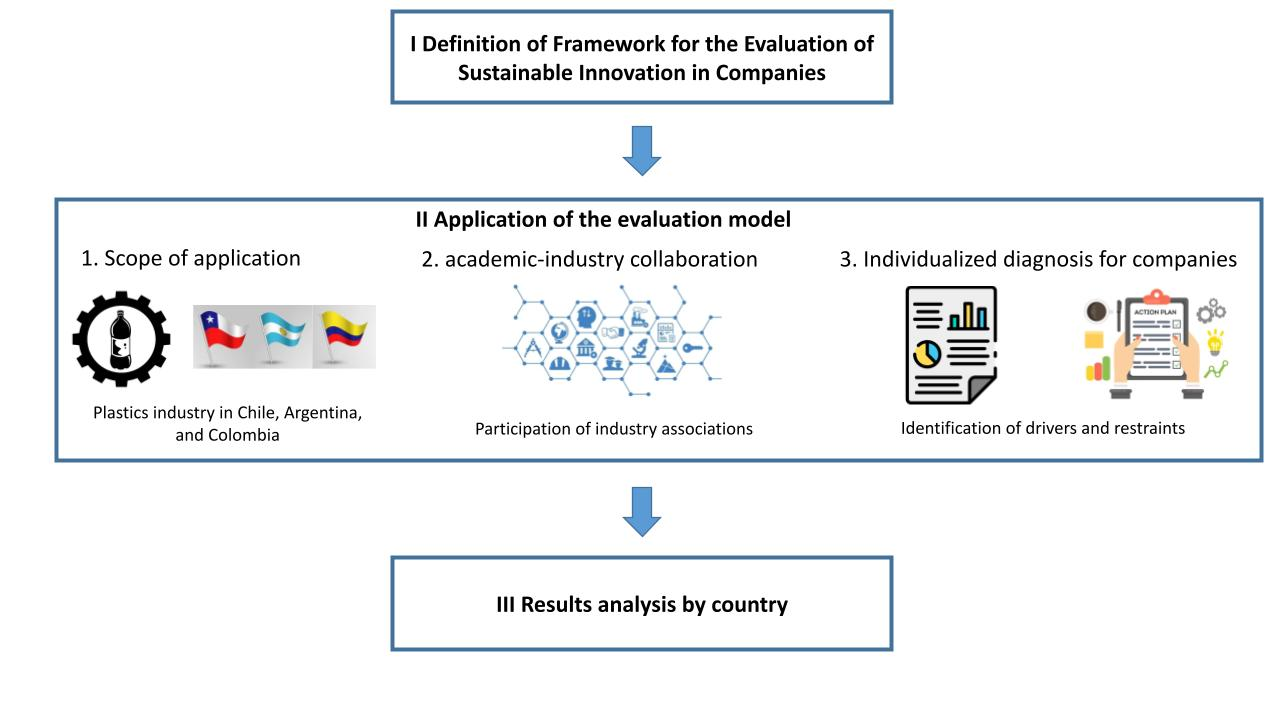
\includegraphics[width=0.9\linewidth,height=\textheight,keepaspectratio]{figures/1.3/01-Methodology.jpg}

}

\caption{\label{fig-1}Three-stage methodology.}

\end{figure}%

\section{I. Definition of framework}\label{i.-definition-of-framework}

In the framework of a master's thesis in engineering sciences,
specializing in industrial engineering at the University of Santiago de
Chile, a conceptual model was developed to evaluate the sustainable
innovation capabilities of companies in the plastics sector.

Following an exhaustive literature review of existing models for
assessing corporate innovation capabilities
(\citeproc{ref-bhatti2023}{Bhatti et al., 2023};
\citeproc{ref-garcia-pozo2016}{García-Pozo et al., 2016};
\citeproc{ref-ortega-lapiedra2019}{Ortega-Lapiedra et al., 2019};
\citeproc{ref-scarpellini2019}{Scarpellini et al., 2019}), and a
comparative analysis of their respective features, a model was designed
with the following key characteristics:

\begin{enumerate}
\def\labelenumi{\arabic{enumi}.}
\tightlist
\item
  Based on best practices identified in the literature and industrial
  experience.
\item
  Structured as a multi-criteria framework to capture different
  dimensions of sustainable innovation.
\item
  Applying a maturity grid evaluation method to assess the level of
  capability development within each company.
\end{enumerate}

This approach draws not only on theoretical insights from previous
studies but also on the practical experience of the \emph{Université de
Lorraine and the Universidad de Santiago de Chile} in developing
management indicators for SMEs (\citeproc{ref-galvez2013}{Galvez et al.,
2013}; \citeproc{ref-munoz2022}{Muñoz et al., 2022}).\\

The identification of good practices (\citeproc{ref-galvez2018}{Galvez
et al., 2018}) serves as the foundation for understanding the internal
functioning of companies, allowing the recognition of key activities and
routines that support the implementation of sustainable innovation
projects. From the literature review, an initial list of potential
practices was compiled and subsequently refined through iteration,
ensuring relevance to the specific context of the plastics industry in
Latin America.

As a result, 27 good practices were identified and grouped into four
main pillars representing the core dimensions of sustainable innovation
capability within the plastics sector as illustrated in
Figure~\ref{fig-2}.

\begin{figure}[H]

\centering{

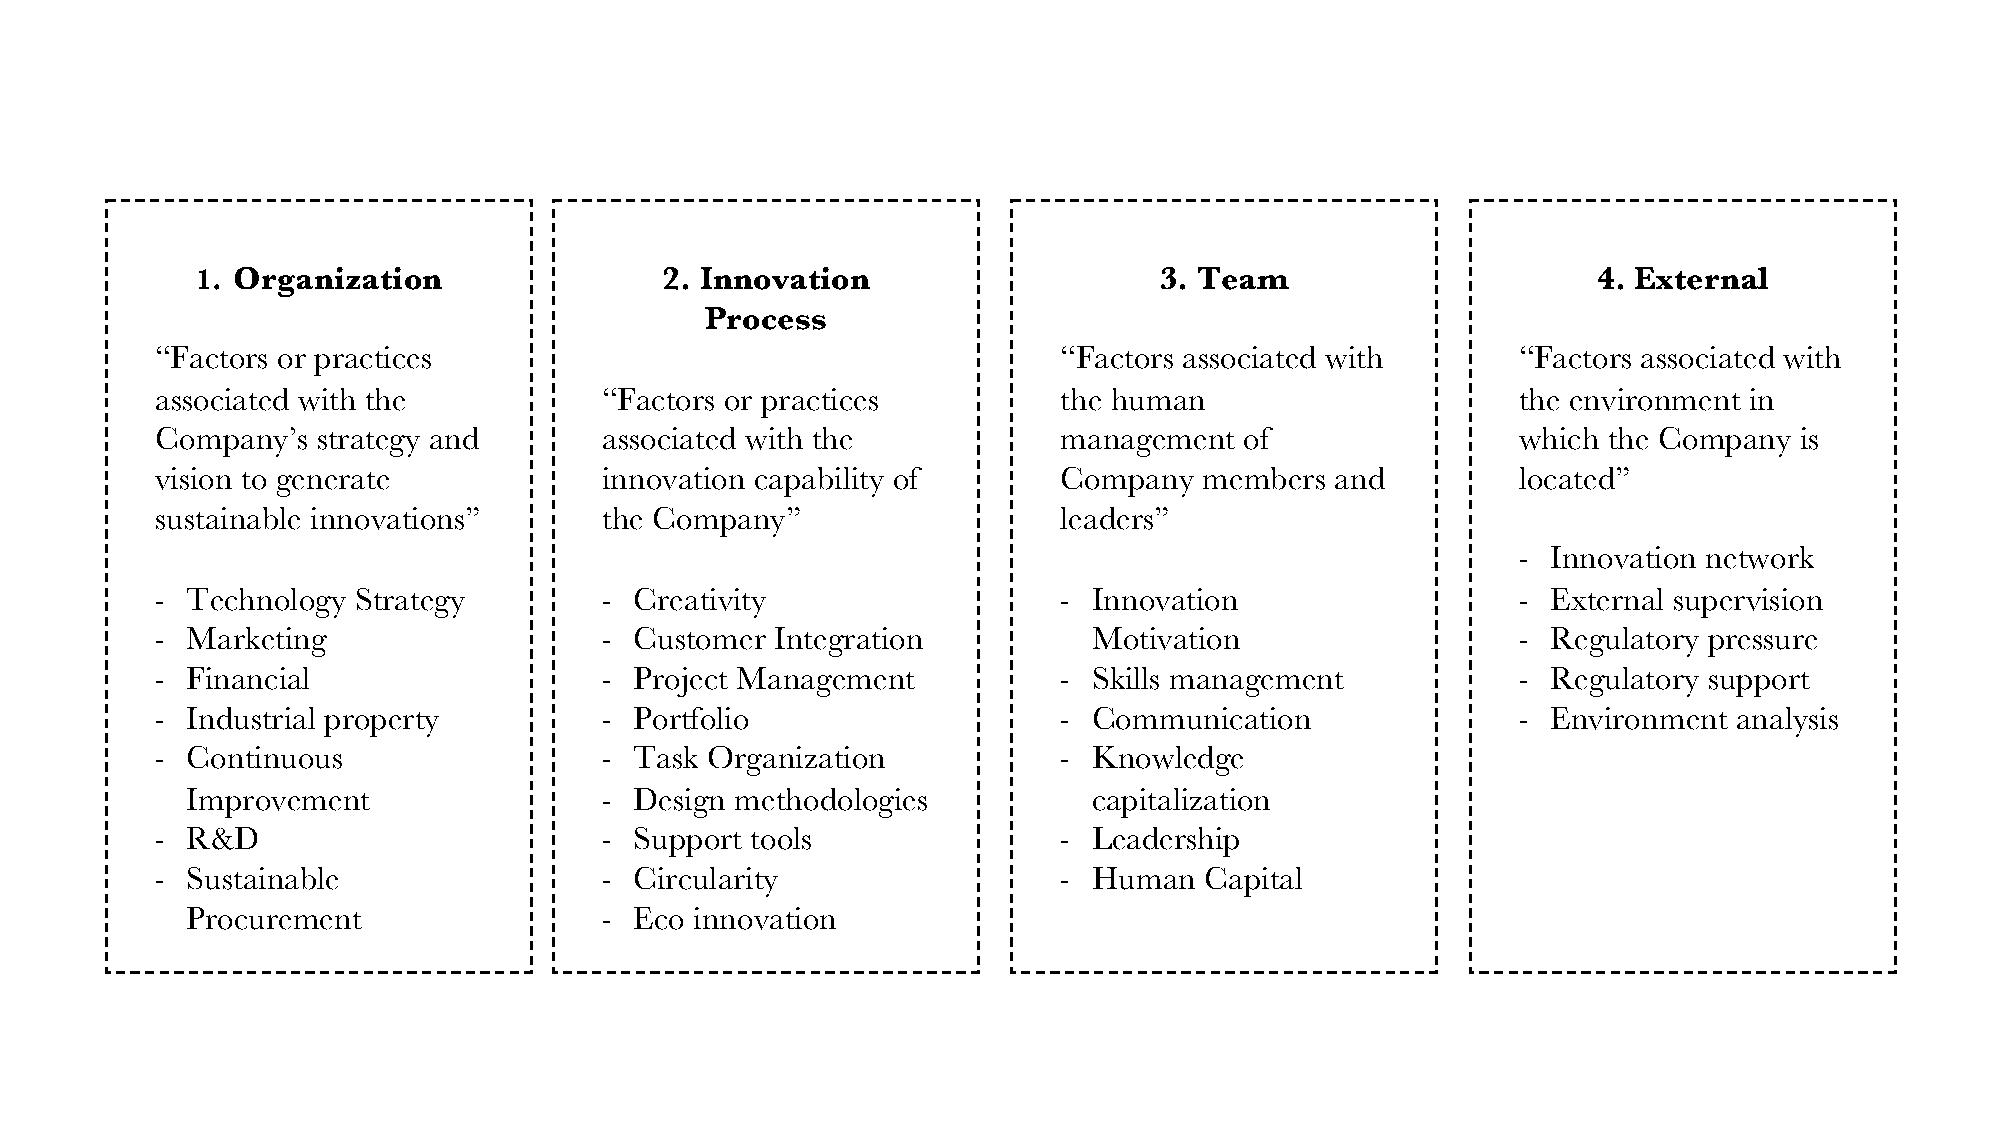
\includegraphics[width=1\linewidth,height=\textheight,keepaspectratio]{figures/1.3/02-framework.pdf}

}

\caption{\label{fig-2}Main pillars of the sustainable innovation
capability.}

\end{figure}%

The first pillar represents practices associated with the organization
of the company, considering aspects such as strategy, financing,
intellectual property, among others (\citeproc{ref-bhatti2023}{Bhatti et
al., 2023}). The second pillar focuses on practices that support the
innovation process from divergence (idea creation) to convergence
(design and prototyping) (\citeproc{ref-monteiro2024}{Monteiro et al.,
2024}; \citeproc{ref-severo2017}{Severo et al., 2017}). The third pillar
refers to the work team, analyzing competencies, leadership, and
communication in the company's operations
(\citeproc{ref-ortega-lapiedra2019}{Ortega-Lapiedra et al., 2019}).
Finally, the fourth pillar evaluates how the company relates to the
outside world in terms of competition analysis, customers, regulatory
aspects, among others (\citeproc{ref-li2021a}{Li et al., 2021}). The
definition of each factor is presented in the following
Table~\ref{tbl-1}.

\begin{landscape}

\begingroup\fontsize{11}{13}\selectfont

\begin{longtable}[t]{>{\centering\arraybackslash}p{1cm}>{\centering\arraybackslash}p{1cm}>{\raggedright\arraybackslash}p{3cm}>{\raggedright\arraybackslash}p{14cm}}

\caption{\label{tbl-1}Definition of the good practices in the
implementation of sustainable innovation projects.}

\tabularnewline

\toprule
\begingroup\fontsize{11}{13}\selectfont \cellcolor{Naranja}{\textcolor{white}{\textbf{Group}}}\endgroup & \begingroup\fontsize{11}{13}\selectfont \cellcolor{Naranja}{\textcolor{white}{\textbf{Acro.}}}\endgroup & \begingroup\fontsize{11}{13}\selectfont \cellcolor{Naranja}{\textcolor{white}{\textbf{Factors}}}\endgroup & \begingroup\fontsize{11}{13}\selectfont \cellcolor{Naranja}{\textcolor{white}{\textbf{Definition}}}\endgroup\\
\midrule
\endfirsthead
\multicolumn{4}{@{}l}{\textit{(continued)}}\\
\toprule
\begingroup\fontsize{11}{13}\selectfont \cellcolor{Naranja}{\textcolor{white}{\textbf{Group}}}\endgroup & \begingroup\fontsize{11}{13}\selectfont \cellcolor{Naranja}{\textcolor{white}{\textbf{Acro.}}}\endgroup & \begingroup\fontsize{11}{13}\selectfont \cellcolor{Naranja}{\textcolor{white}{\textbf{Factors}}}\endgroup & \begingroup\fontsize{11}{13}\selectfont \cellcolor{Naranja}{\textcolor{white}{\textbf{Definition}}}\endgroup\\
\midrule
\endhead

\endfoot
\bottomrule
\endlastfoot
 & A.E & Analysis of the Environment & This corresponds to the strategic assessment of external factors (economic, social, technological, and regulatory) that influence sustainable innovation. It considers not only regulation, but also the market, consumer trends, competition, and changes in demand.\\
\cmidrule{2-4}\nopagebreak
 & I.N & Innovation Networks & This refers to strategic collaborations between companies, universities, research centers, and government agencies. They facilitate the exchange of knowledge, technologies, and best practices that promote sustainable innovation. This component focuses on interaction and cooperation within the innovation ecosystem.\\
\cmidrule{2-4}\nopagebreak
 & E.S & External Supervision & This refers to the set of control, audit, and regulatory mechanisms applied by government agencies, industry associations, and the market. Its purpose is to ensure that companies comply with environmental regulations and sustainability standards.\\
\cmidrule{2-4}\nopagebreak
 & R.P & Regulatory Pressure & This corresponds to regulations and legal requirements that oblige companies to adopt more sustainable practices. It can manifest itself in environmental restrictions, energy efficiency requirements, or emission reduction targets. It represents the mandatory side of regulation, i.e., the rules that companies must follow in order to operate within the law.\\
\cmidrule{2-4}\nopagebreak
\multirow[t]{-5}{1cm}[4\dimexpr\aboverulesep+\belowrulesep+\cmidrulewidth]{\centering\arraybackslash \rotatebox{90}{External Factors}} & R.S & Regulatory Support & This refers to government policies and programs designed to promote sustainable innovation, such as financing, advice, and eco-certifications. It is the counterpart to regulatory pressure, as it represents an incentive rather than an obligation.\\
\cmidrule{1-4}\pagebreak[0]
 & I.E.C & Internal and External Communication & It corresponds to the process by which the company facilitates the exchange of information among work teams, fostering collaboration and the integration of knowledge in initiatives based on sustainable innovation.\\
\cmidrule{2-4}\nopagebreak
 & H.C & Human Capital & It is defined as the set of knowledge, skills, experience and capabilities acquired by employees, which directly influence the company's ability to develop innovations that encompass the triple bottom line.\\
\cmidrule{2-4}\nopagebreak
 & M.I & Motivation for Innovation & This refers to the level of commitment, enthusiasm, and willingness of employees to get involved in developing innovative solutions. It is not just about having technical knowledge, but about wanting to actively apply it to the sustainable transformation of the company.\\
\cmidrule{2-4}\nopagebreak
 & S.M & Skills Management & This refers to the set of strategies and processes that the company implements to develop, update, and manage the team's skills, ensuring that they are aligned with the needs of innovation.\\
\cmidrule{2-4}\nopagebreak
 & C.K & Capitalization of Knowledge & This refers to the process of documenting, storing, and reusing the knowledge generated within the company, ensuring that best practices and lessons learned in innovation are accessible and applicable in the future.\\
\cmidrule{2-4}\nopagebreak
\multirow[t]{-6}{1cm}[5\dimexpr\aboverulesep+\belowrulesep+\cmidrulewidth]{\centering\arraybackslash \rotatebox{90}{Team factors}} & LEA & Leadership & Refers to the ability of executives and managers to promote sustainability, guide teams toward strategic innovation goals, and efficiently manage human capital.\\
\cmidrule{1-4}\pagebreak[0]
 & I.P & Innovation Portfolio & This refers to the strategic management of innovation projects, ensuring their alignment with the company's vision. Managing the project portfolio allows you to control the pace of new releases, avoid resource congestion, and not focus exclusively on the short term at the expense of the long term.\\
\cmidrule{2-4}\nopagebreak
 & E.P.P & Eco-innovation in products and processes & This refers to the implementation of technological and organizational innovations that improve a company's environmental performance, optimizing the use of natural resources and reducing the environmental impacts of industrial production.\\
\cmidrule{2-4}\nopagebreak
 & S.T & Support Tools & This refers to the use of technologies and systems that facilitate the implementation of sustainable innovations, such as simulation software, modeling, and data analysis tools to assess the viability of new processes.\\
\cmidrule{2-4}\nopagebreak
 & D.M & Design Methodologies & Refers to design strategies used to develop sustainable products and processes, including eco-design, life cycle assessment (LCA), and waste minimization strategies.\\
\cmidrule{2-4}\nopagebreak
 & T.A & Task Organization & This refers to the efficient structuring of activities within innovation processes, ensuring the optimal allocation of resources, time, and responsibilities in sustainable development projects.\\
\cmidrule{2-4}\nopagebreak
 & I.P.M & Innovation Project Management & It refers to the management of resources, deadlines, risks, and objectives in the development of innovation projects, ensuring their effective execution and alignment with sustainability principles.\\
\cmidrule{2-4}\nopagebreak
 & CIRC & Circularity & This corresponds to strategies for recycling, reuse, and reduction in production processes, together with the use of metrics to evaluate the efficiency of these changes.\\
\cmidrule{2-4}\nopagebreak
 & C.I & Customer Integration & It refers to incorporating customer feedback and needs into the development of innovations, ensuring that products and processes meet market expectations and encourage the adoption of sustainable solutions.\\
\cmidrule{2-4}\nopagebreak
\multirow[t]{-9}{1cm}[8\dimexpr\aboverulesep+\belowrulesep+\cmidrulewidth]{\centering\arraybackslash \rotatebox{90}{Innovation Process}} & CREA & Creativity & This refers to the generation of innovative ideas that enable the transformation of products, processes, and business models into more sustainable, efficient solutions with a lower environmental impact.\\
\cmidrule{1-4}\pagebreak[0]
 & MARK & Marketing & It refers to communication and positioning strategies to differentiate sustainable products and generate value in the market.\\
\cmidrule{2-4}\nopagebreak
 & F.M & Financial Management & It corresponds to the administration of financial resources to fund sustainable innovation projects and responsible purchasing.\\
\cmidrule{2-4}\nopagebreak
 & I.P2 & Intellectual Property & This refers to the protection of innovations and technologies that contribute to the sustainable competitiveness of the company.\\
\cmidrule{2-4}\nopagebreak
 & C.I3 & Continuous Improvement & This involves the constant evaluation and optimization of processes to improve efficiency and reduce environmental impacts.\\
\cmidrule{2-4}\nopagebreak
 & R.D & Research and Development & Refers to the development of new technologies, products, and processes aimed at sustainable innovation.\\
\cmidrule{2-4}\nopagebreak
 & T.S & Technological Strategy & This involves integrating advanced technologies to optimize production and reduce environmental impacts within the organization.\\
\cmidrule{2-4}\nopagebreak
\multirow[t]{-7}{1cm}[6\dimexpr\aboverulesep+\belowrulesep+\cmidrulewidth]{\centering\arraybackslash \rotatebox{90}{Organization}} & S.P.S.P & Sustainable Purchasing in the Supply Chain & Refers to procurement and logistics management strategies based on environmental, social, and economic criteria to reduce negative impacts in the supply chain and improve sustainable competitiveness.\\*

\end{longtable}

\endgroup{}

\end{landscape}

Once the practices were defined, the model was structured using the
Analytic Hierarchy Process (AHP) multi-criteria method. This approach
was selected for its hierarchical structure and its ability to calculate
a weighting vector that determines the relative importance of the
practices comprising the model. Figure~\ref{fig-3} shows the final
structure of the proposed model.

\begin{figure}[H]

\centering{

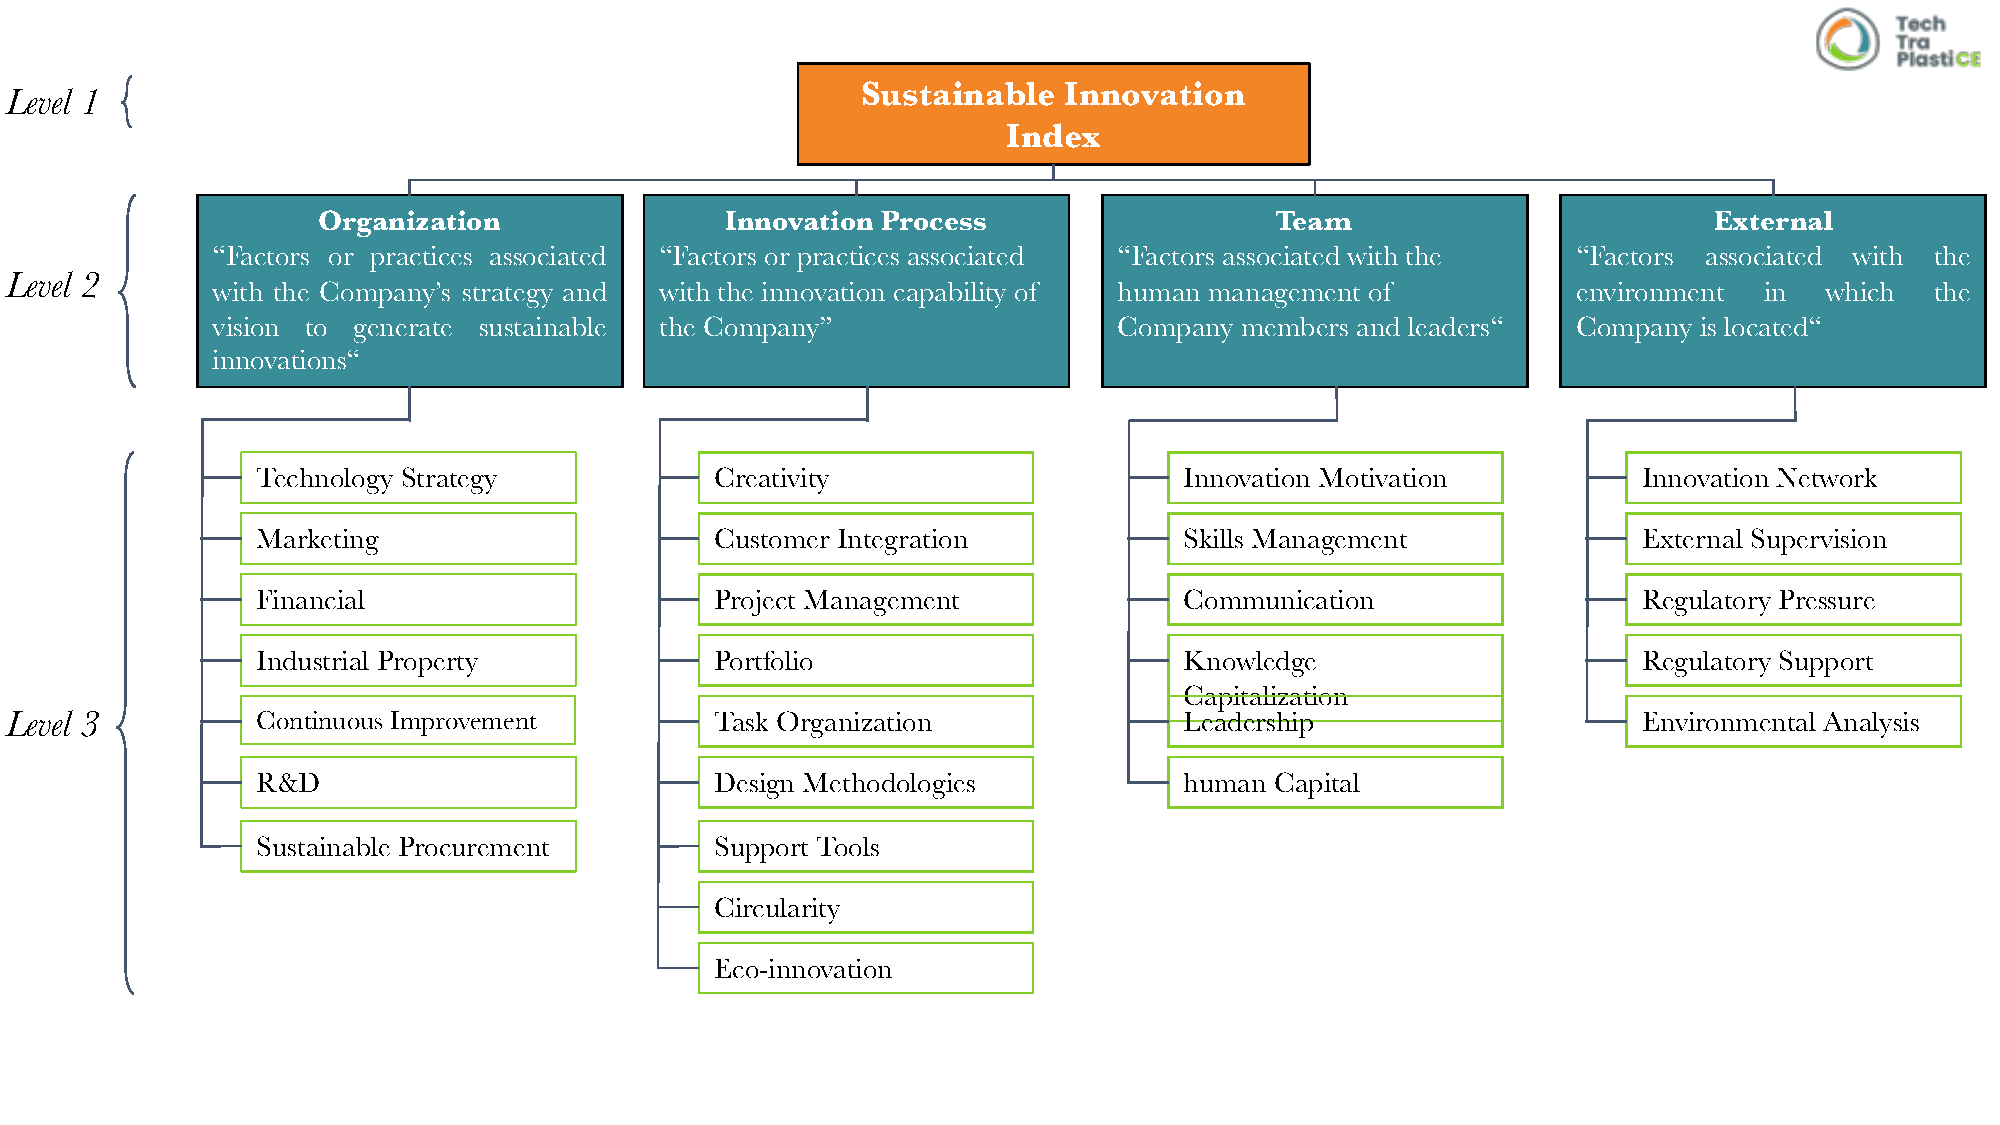
\includegraphics[width=0.9\linewidth,height=\textheight,keepaspectratio]{figures/1.3/03-Model.pdf}

}

\caption{\label{fig-3}Final structure of the model.}

\end{figure}%

The hierarchy structure of the model is divided into three levels. At
the first level, the global sustainable innovation index is found, which
represents the company's capability to implement this type of project.
At the intermediate level are placed the four pillars described in the
evaluation framework. At the lowest level are the practices that
characterize each pillar. These practices represent activities and
routines that the company can implement to improve its capacity for
sustainable innovation. In other words, the company's overall capability
is determined by its performance across these practices.

According to the functioning of the multi-criteria structure based on
the AHP method, the evaluation is applied at the lowest level of the
hierarchical structure, that is, to the practices. Each practice
represents different activities undertaken by the company, allowing it
to evaluate its performance. This performance depends on factors such
expertise, human capital, methods and tools employed, among other
resources. The evaluation approach adopted is the maturity grid, a
widely used method for assessing the performance of internal
organizational activities or practices through the definition of
progressive levels of maturity.

The definition of these grids is essential, as it allows the assessment
to be adapted to the specific type of sustainable innovation. The grid
reflects how companies implement practices and identify the resources
and actions required to achieve triple-impact innovations. Each practice
is evaluated using a five-level maturity grid as illustrated in
Table~\ref{tbl-maturity}. For example, the grid developed for the
\emph{innovation networks} (\emph{I.N}) practice illustrates this
approach. Each good practice is related to a precise level of maturity.
For the complete questionnaire refer to the Annex
Section~\ref{sec-instrument}.

The main advantage of using maturity grids lies in their ability to
reduce response subjectivity, since each level is defined according to
observable phenomena. In addition, they facilitate the development of
targeted improvement plans, as the five maturity levels for each
practice are available. Therefore, if the company is positioned at an
intermediate level for a given practice, it becomes evident which
actions must be undertaken to reach the next level.

\begin{table}

\caption{\label{tbl-maturity}Maturity grid example for innovation
networks --IN-.}

\centering{

\centering\begingroup\fontsize{11}{13}\selectfont

\begin{tabular}[t]{>{\raggedright\arraybackslash}p{3cm}>{\raggedright\arraybackslash}p{3cm}>{\raggedright\arraybackslash}p{3cm}>{\raggedright\arraybackslash}p{3cm}>{\raggedright\arraybackslash}p{3cm}}
\toprule
\begingroup\fontsize{12}{14}\selectfont \cellcolor{Naranja}{\textcolor{white}{\textbf{Level 1}}}\endgroup & \begingroup\fontsize{12}{14}\selectfont \cellcolor{Naranja}{\textcolor{white}{\textbf{Level 2}}}\endgroup & \begingroup\fontsize{12}{14}\selectfont \cellcolor{Naranja}{\textcolor{white}{\textbf{Level 3}}}\endgroup & \begingroup\fontsize{12}{14}\selectfont \cellcolor{Naranja}{\textcolor{white}{\textbf{Level 4}}}\endgroup & \begingroup\fontsize{12}{14}\selectfont \cellcolor{Naranja}{\textcolor{white}{\textbf{Level 5}}}\endgroup\\
\midrule
The company works only with internal resources & The company works with customers or suppliers. & The company typically uses external resources privileging two of the three impacts & The company regularly engages in collaborative projects that are selected according to its sustainable innovation strategy. & The company follows an openness strategy with leading actors in sustainability.\\
\bottomrule
\end{tabular}
\endgroup{}

}

\end{table}%

The development of this model for assessing the sustainable innovation
capability of companies was presented by a master's student at the IAMOT
(International Association for Management of Technology) 2025
international conference in Canada
(\citeproc{ref-astudillo2025}{Astudillo et al., 2025}).

\section{II. Application of evaluation
Model}\label{ii.-application-of-evaluation-model}

To implement the proposed assessment model in partner companies, a
dedicated tool was developed. It consists of a survey comprising 27
questions structured according to the maturity grid approach, where one
maturity grid question corresponds to each of the 27 practices defined
in the model. The survey was made available online to facilitate
participation and data collection from companies.

\subsection{Scope of Application}\label{scope-of-application}

Within the objective to evaluate partner companies across the three
Latin American countries participating in the project and ensure
comparability, a set of basic characteristics was defined to guide the
selection of companies in each country. The assessment primarily targets
companies within the plastics industry, with a goal of engaging at
\emph{least ten companies per country}. A socialization of the task was
made on June 09/20025 at the general monthly meeting of the
TechTraPlastiCE consortium as presented in Figure~\ref{fig-4}.

\begin{figure}[H]

\centering{

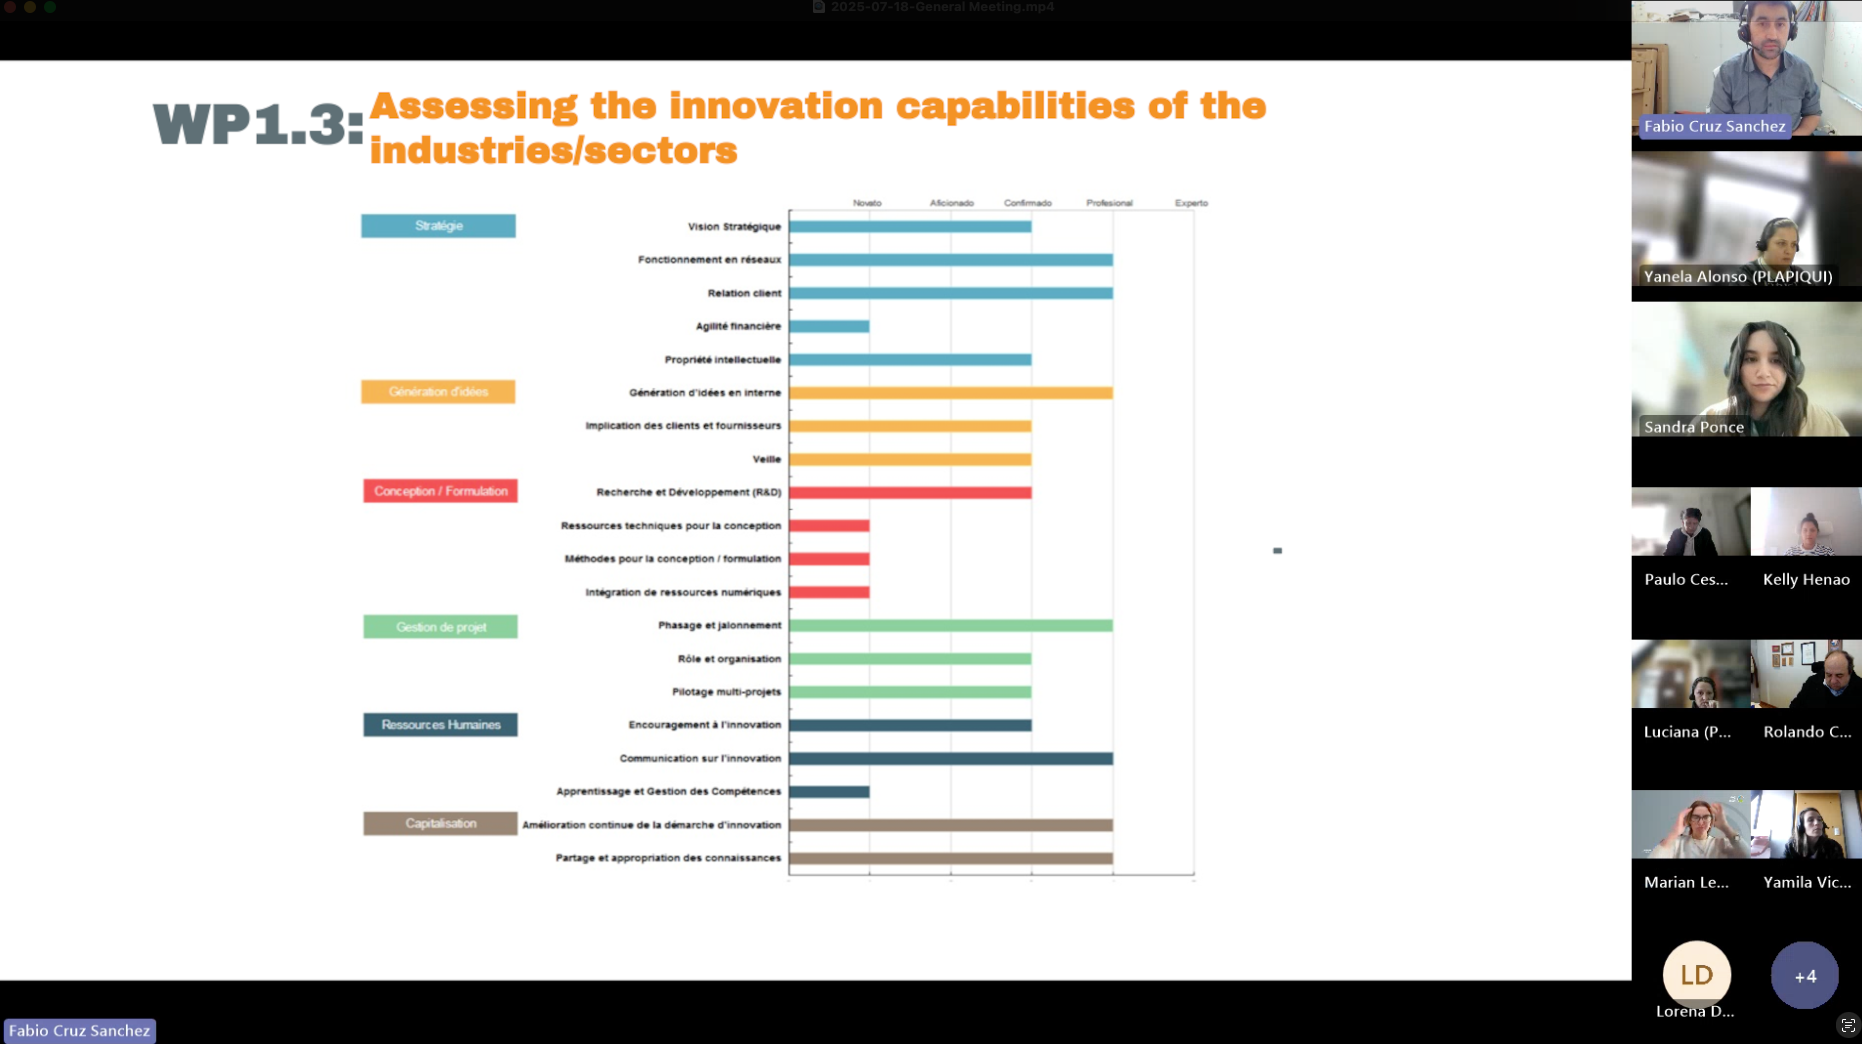
\includegraphics[width=0.8\linewidth,height=\textheight,keepaspectratio]{figures/1.3/Socialization.png}

}

\caption{\label{fig-4}Socialization of the task on General Meeting June
09/2025.}

\end{figure}%

\subsection{Academia-industry collaboration
strategy}\label{academia-industry-collaboration-strategy}

The success of the survey implementation is directly linked to the
strength of the relationship between academia and industry. To promote
this collaboration, two strategies were adopted: (1) leveraging existing
connections within the university environment and (2) engaging trade
associations in the plastics industry. In the first strategy, the
partner universities that already have experience in projects involving
companies from this sector, helped to foster trust in their work and,
consequently, increased the willingness of these companies to
participate. The second strategy aims to expand the scope of action and
engage a larger number of companies through intermediaries,
specifically, trade associations within the plastics industry. For
instance, in Colombia this involves the participation of
\textbf{ACOPLASTICOS} (\url{https://acoplasticos.org/}), and in Chile
with \textbf{ASIPLA} (\url{https://asipla.cl/}). These associations
serve as facilitators by promoting participation in the survey among
their member companies.

For both strategies, explanatory manuals are being developed to support
understanding of the model and to facilitate the application of the
survey. Additionally, a designated contact person is made available to
address any questions or requests for clarification from participating
companies.

\subsection{Individualized diagnosis for
companies}\label{individualized-diagnosis-for-companies}

Once the questionnaire is completed and analysed, each company receives
a diagnostic report assessing its sustainable innovation capabilities.
This report presents the companies' overall index, along with detailed
profiles organized by pillar and by practice, thereby identifying
specific strengths and weaknesses. The diagnosis enables companies to
better understand the activities that influence their potential to
implement sustainable innovation projects.

Companies that have already developed sustainable innovation projects
can use the report's findings to standardize their practices, thereby
enhancing their capacity to replicate and scale similar projects.
Furthermore, companies interested in developing an improvement plan are
invited to contact the research team to schedule a follow-up meeting.

The entire process of conducting the survey and delivering diagnostic
reports to companies was conducted by a \emph{master's student from the
University of Santiago, Chile, and a master's student from the National
University of Colombia, with support from undergraduate students who
provided methodological and technical assistance to the participating
companies}.

The final stage of the methodology involves the analysis of the results,
which is presented in the following section.

\chapter{Results}\label{results}

This section presents the results of the survey, organized by country.
First, a descriptive analysis of the responses is conducted for each
country, categorized by company size. Subsequently, a cluster analysis
is performed to identify company profiles based on the evaluated
factors, allowing for the characterization of their capacity to
implement sustainable innovations.

\section{Descriptive Analysis of the
Results}\label{descriptive-analysis-of-the-results}

The distribution of participating companies by size is summarized in
Table Table~\ref{tbl-summary}. For the purposes of this study, company
size was categorized according to the number of employees, as follows:

\begin{itemize}
\tightlist
\item
  Micro enterprises: 1--9 employees
\item
  Small enterprises: 10--49 employees
\item
  Medium-sized enterprises: 50--199 employees
\item
  Large enterprises: 200 or more employees
\end{itemize}

Between June 15, 2025, and October 15, 2025, a total of 68 enterprises
from Argentina, Chile, and Colombia participated in the survey and
completed the evaluation instrument. The analysis reveals that
medium-sized and large companies represent the majority of participants
across the three countries, accounting for approximately 58.8\% of the
total sample. In Colombia, these companies constitute around 63.9\% of
national participants and 33.8\% of the overall sample. In Argentina,
medium and large firms make up about 60\% of national participants,
corresponding to 17.6\% of the total sample. Finally, in Chile,
companies of similar size represent 41.7\% of national participants and
7.4\% of the total sample.

\begin{table}

\caption{\label{tbl-summary}Distribution of participating companies by
size}

\centering{

\centering\begingroup\fontsize{11}{13}\selectfont

\begin{tabular}[t]{>{\centering\arraybackslash}p{3cm}>{\centering\arraybackslash}p{3cm}>{\centering\arraybackslash}p{3cm}>{\centering\arraybackslash}p{3cm}}
\toprule
\begingroup\fontsize{12}{14}\selectfont \cellcolor{Naranja}{\textcolor{white}{\textbf{Country}}}\endgroup & \begingroup\fontsize{12}{14}\selectfont \cellcolor{Naranja}{\textcolor{white}{\textbf{Size}}}\endgroup & \begingroup\fontsize{12}{14}\selectfont \cellcolor{Naranja}{\textcolor{white}{\textbf{\# Enterprises}}}\endgroup & \begingroup\fontsize{12}{14}\selectfont \cellcolor{Naranja}{\textcolor{white}{\textbf{\% per country}}}\endgroup\\
\midrule
 & Large & 7 & 35.00\\
\cmidrule{2-4}
 & Medium & 5 & 25.00\\
\cmidrule{2-4}
 & Small & 3 & 15.00\\
\cmidrule{2-4}
\multirow[t]{-4}{3cm}[3\dimexpr\aboverulesep+\belowrulesep+\cmidrulewidth]{\centering\arraybackslash Argentina} & Micro & 5 & 25.00\\
\cmidrule{1-4}
 & Large & 2 & 16.67\\
\cmidrule{2-4}
 & Medium & 3 & 25.00\\
\cmidrule{2-4}
 & Small & 4 & 33.33\\
\cmidrule{2-4}
\multirow[t]{-4}{3cm}[3\dimexpr\aboverulesep+\belowrulesep+\cmidrulewidth]{\centering\arraybackslash Chile} & Micro & 3 & 25.00\\
\cmidrule{1-4}
 & Large & 11 & 30.56\\
\cmidrule{2-4}
 & Medium & 12 & 33.33\\
\cmidrule{2-4}
 & Small & 6 & 16.67\\
\cmidrule{2-4}
\multirow[t]{-4}{3cm}[3\dimexpr\aboverulesep+\belowrulesep+\cmidrulewidth]{\centering\arraybackslash Colombia} & Micro & 7 & 19.44\\
\bottomrule
\end{tabular}
\endgroup{}

}

\end{table}%

Figure~\ref{fig-4} illustrates the distribution of participating
enterprises from Colombia, Chile, and Argentina according to company
size. The sample indicates a particularly active participation from
Colombian enterprises, which account for 52.9\% of the total
respondents.

\begin{figure}[H]

\centering{

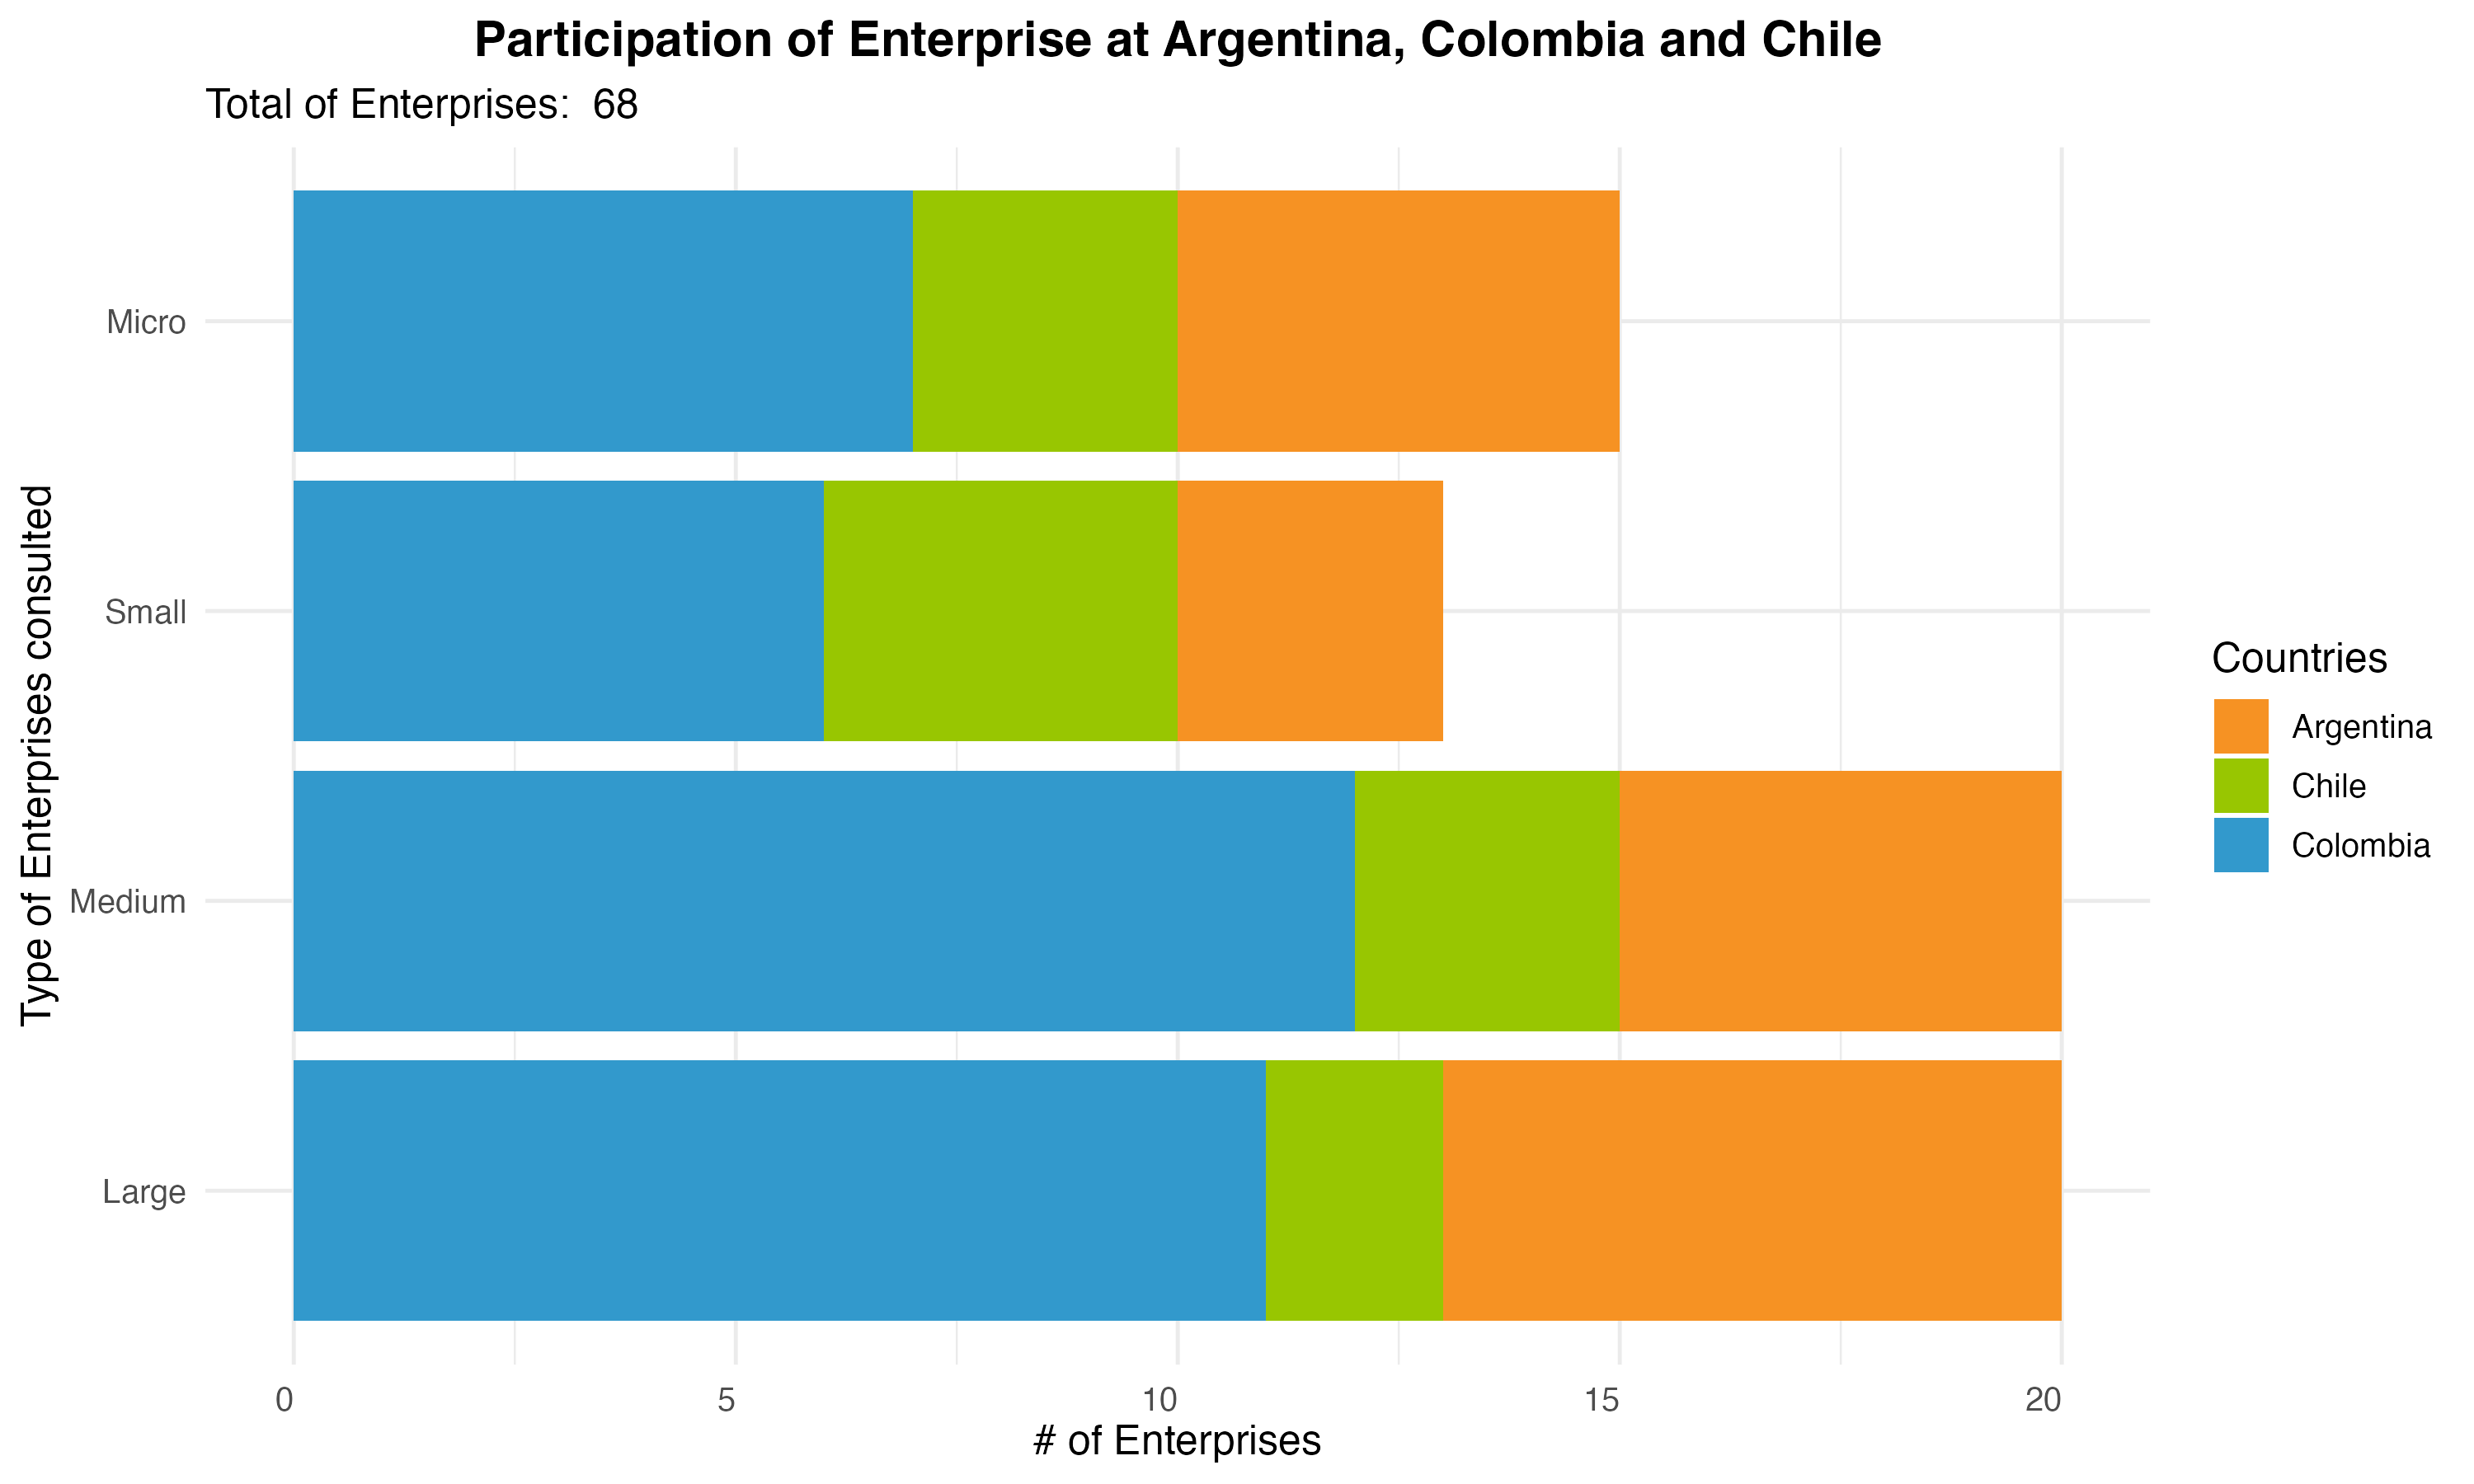
\includegraphics[width=0.9\linewidth,height=\textheight,keepaspectratio]{figures/1.3/Participation.png}

}

\caption{\label{fig-4}Distribution of enterprises by size}

\end{figure}%

In the following section, an analysis by country is made to better
understand the global results.

\section{Analysis by Country}\label{analysis-by-country}

\subsection{Colombia}\label{colombia}

Figure~\ref{fig-Col} presents the results of the average value of the
evaluated practices discrimated by the size of the enterprises at
Colombian enterprises.

\begin{figure}[H]

\centering{

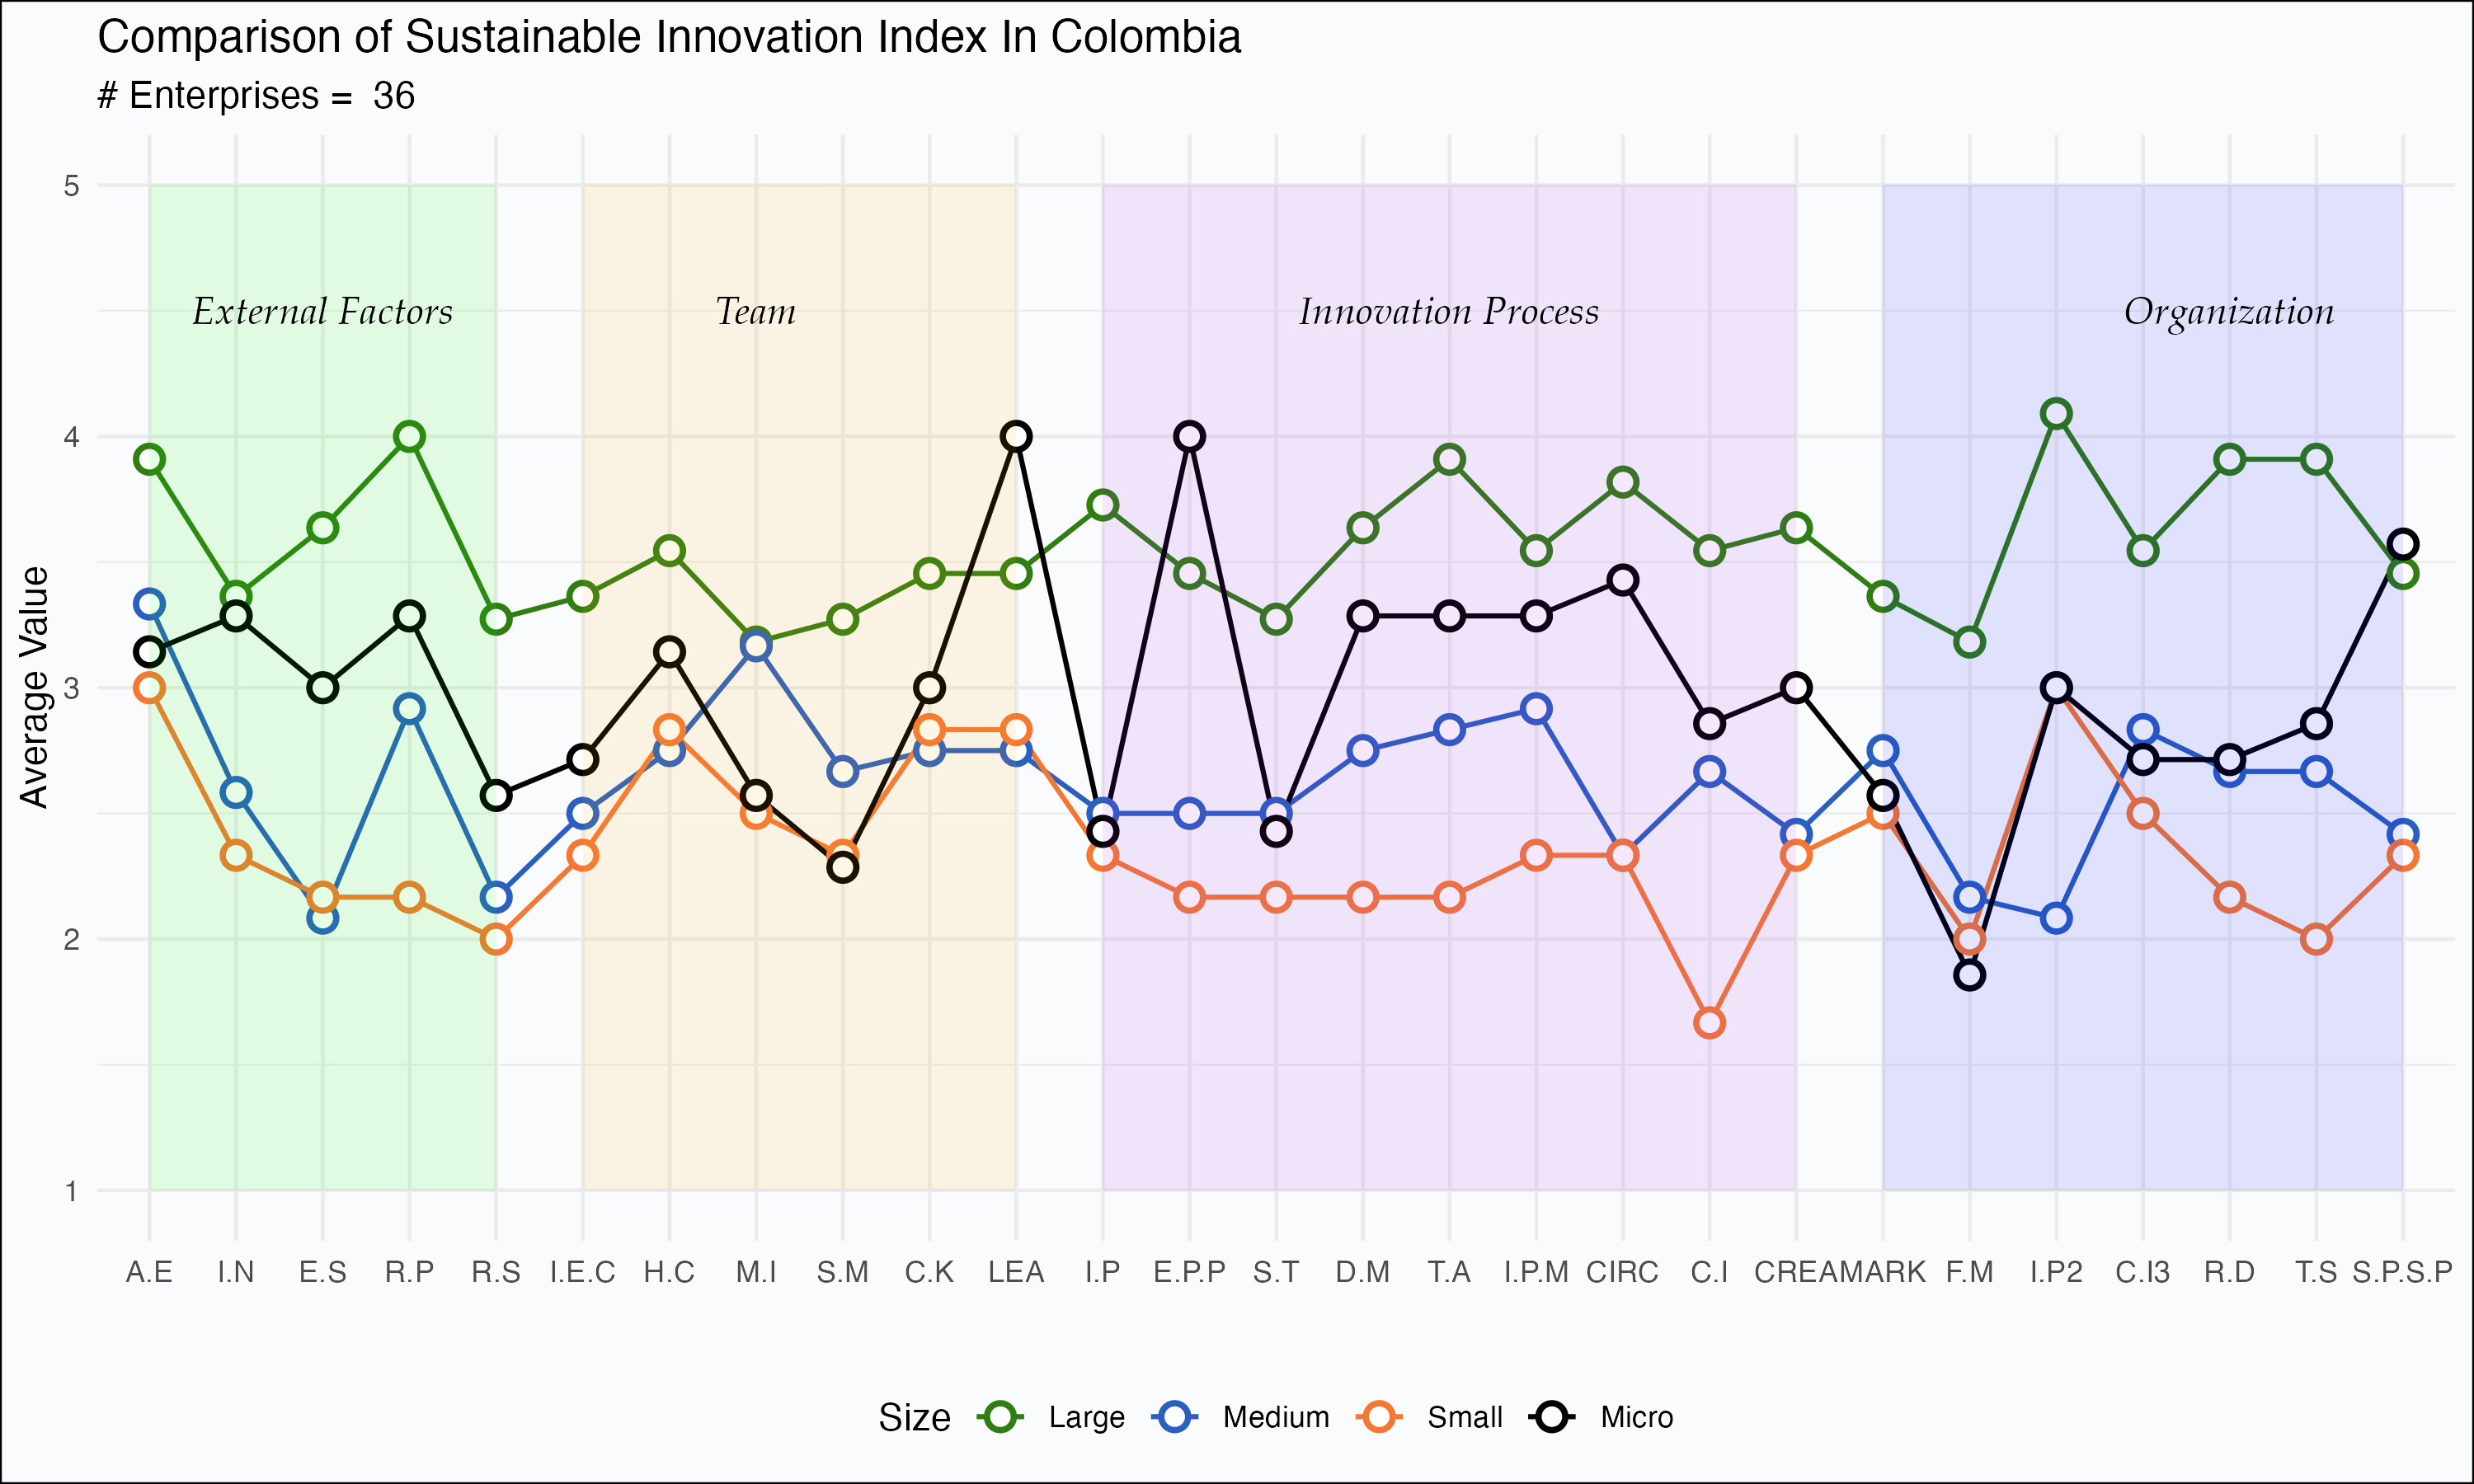
\includegraphics[width=0.9\linewidth,height=\textheight,keepaspectratio]{figures/1.3/Comparison-Colombia.png}

}

\caption{\label{fig-Col}Global Sustainable Innovation index per practice
at Colombia enterprise}

\end{figure}%

In the Colombian context, analysis of the level of maturity in
innovation and business management reveals a landscape where strengths
and weaknesses vary significantly depending on the size of the company,
reflecting the structural diversity and capabilities of the national
productive fabric.

Large companies show the greatest strengths, with an average maturity
level of around 3.6, particularly in \emph{Intellectual Property} (4.5).
Innovation Processes, Organizational management and Team factors, with
values ranging from 3 to 4.5, demonstrating solid structures, clear
technological strategies, and a consolidated culture of continuous
improvement. However, their main weakness lies in financial management
which averages 3.2. Although not critical, this represents an area of
opportunity for improving the financial sustainability of innovation
activities.

Medium-sized companies, with an average maturity level
(\textasciitilde{} 2.6), show partial strengths in some specific
indicators, such as \emph{Analysis of the Environment} (3.75) and
\emph{Motivation for Innovation} (3.3), as well as good results in
certain components of the Innovation Process (\emph{Design
Methodologies, Support Tools, Innovation Project Management, and
Eco-innovation in products and processes}) with values between 3.5 and
4. However, their main weakness lies in a general lack of consistency,
as most indicators remain between 2 and 3, (specially organizational
factors) reflecting an incipient and heterogeneous maturity. In the case
of small enterprises (\textasciitilde2.4) exhibit the lowest levels of
maturity, with few strengths, such as \emph{Analysis of the
Environment}(3) and \emph{Human Capital} (3), and multiple weaknesses in
innovation and organization, \emph{Customer Integration CI} (1.8),
\emph{Financial Management }(2.0), \emph{Research and Development
}(1.9), and \emph{Technological Strategy} (1.8) reflect deficiencies in
technological, financial, and knowledge management capabilities. This
result is to be expected, as small companies normally only plan for the
short term and spend their time solving day-to-day problems, which makes
it difficult to manage sustainable innovation projects that require
greater uncertainty management.

In the case of micro-enterprises (\textasciitilde2.9), there is greater
variability in their assessments. They show some isolated strengths in
External Factors, with values close to 3.5, and in some indicators such
as \emph{Eco-innovation in products and processes }(4.1), but they have
significant weaknesses in \emph{Financial Management }(2),
\emph{Regulatory Support} (2.6), and* Competence Management* (2.6),
suggesting a fragile structure. Due to their size, these companies have
a flexible structure, which favors agility in some processes but hinders
resource support in other activities, which is why there is greater
variability in their practices,

In summary, the analysis shows that Colombia faces a marked gap in
business maturity, where large companies act as poles of development and
innovative leadership, while micro, small, and some medium-sized
companies still need to strengthen their organizational, financial, and
technological capabilities to achieve sustainable and competitive
performance at the national and international levels.

\subsection{Argentina}\label{argentina}

As presented in the Figure~\ref{fig-AR}, the analysis of the level of
maturity in sustainable innovation management in the case of Argentina
reveals a picture of strengths and weaknesses that vary according to
company size, with a general trend toward medium levels of development
in the practices evaluated.

\begin{figure}[H]

\centering{

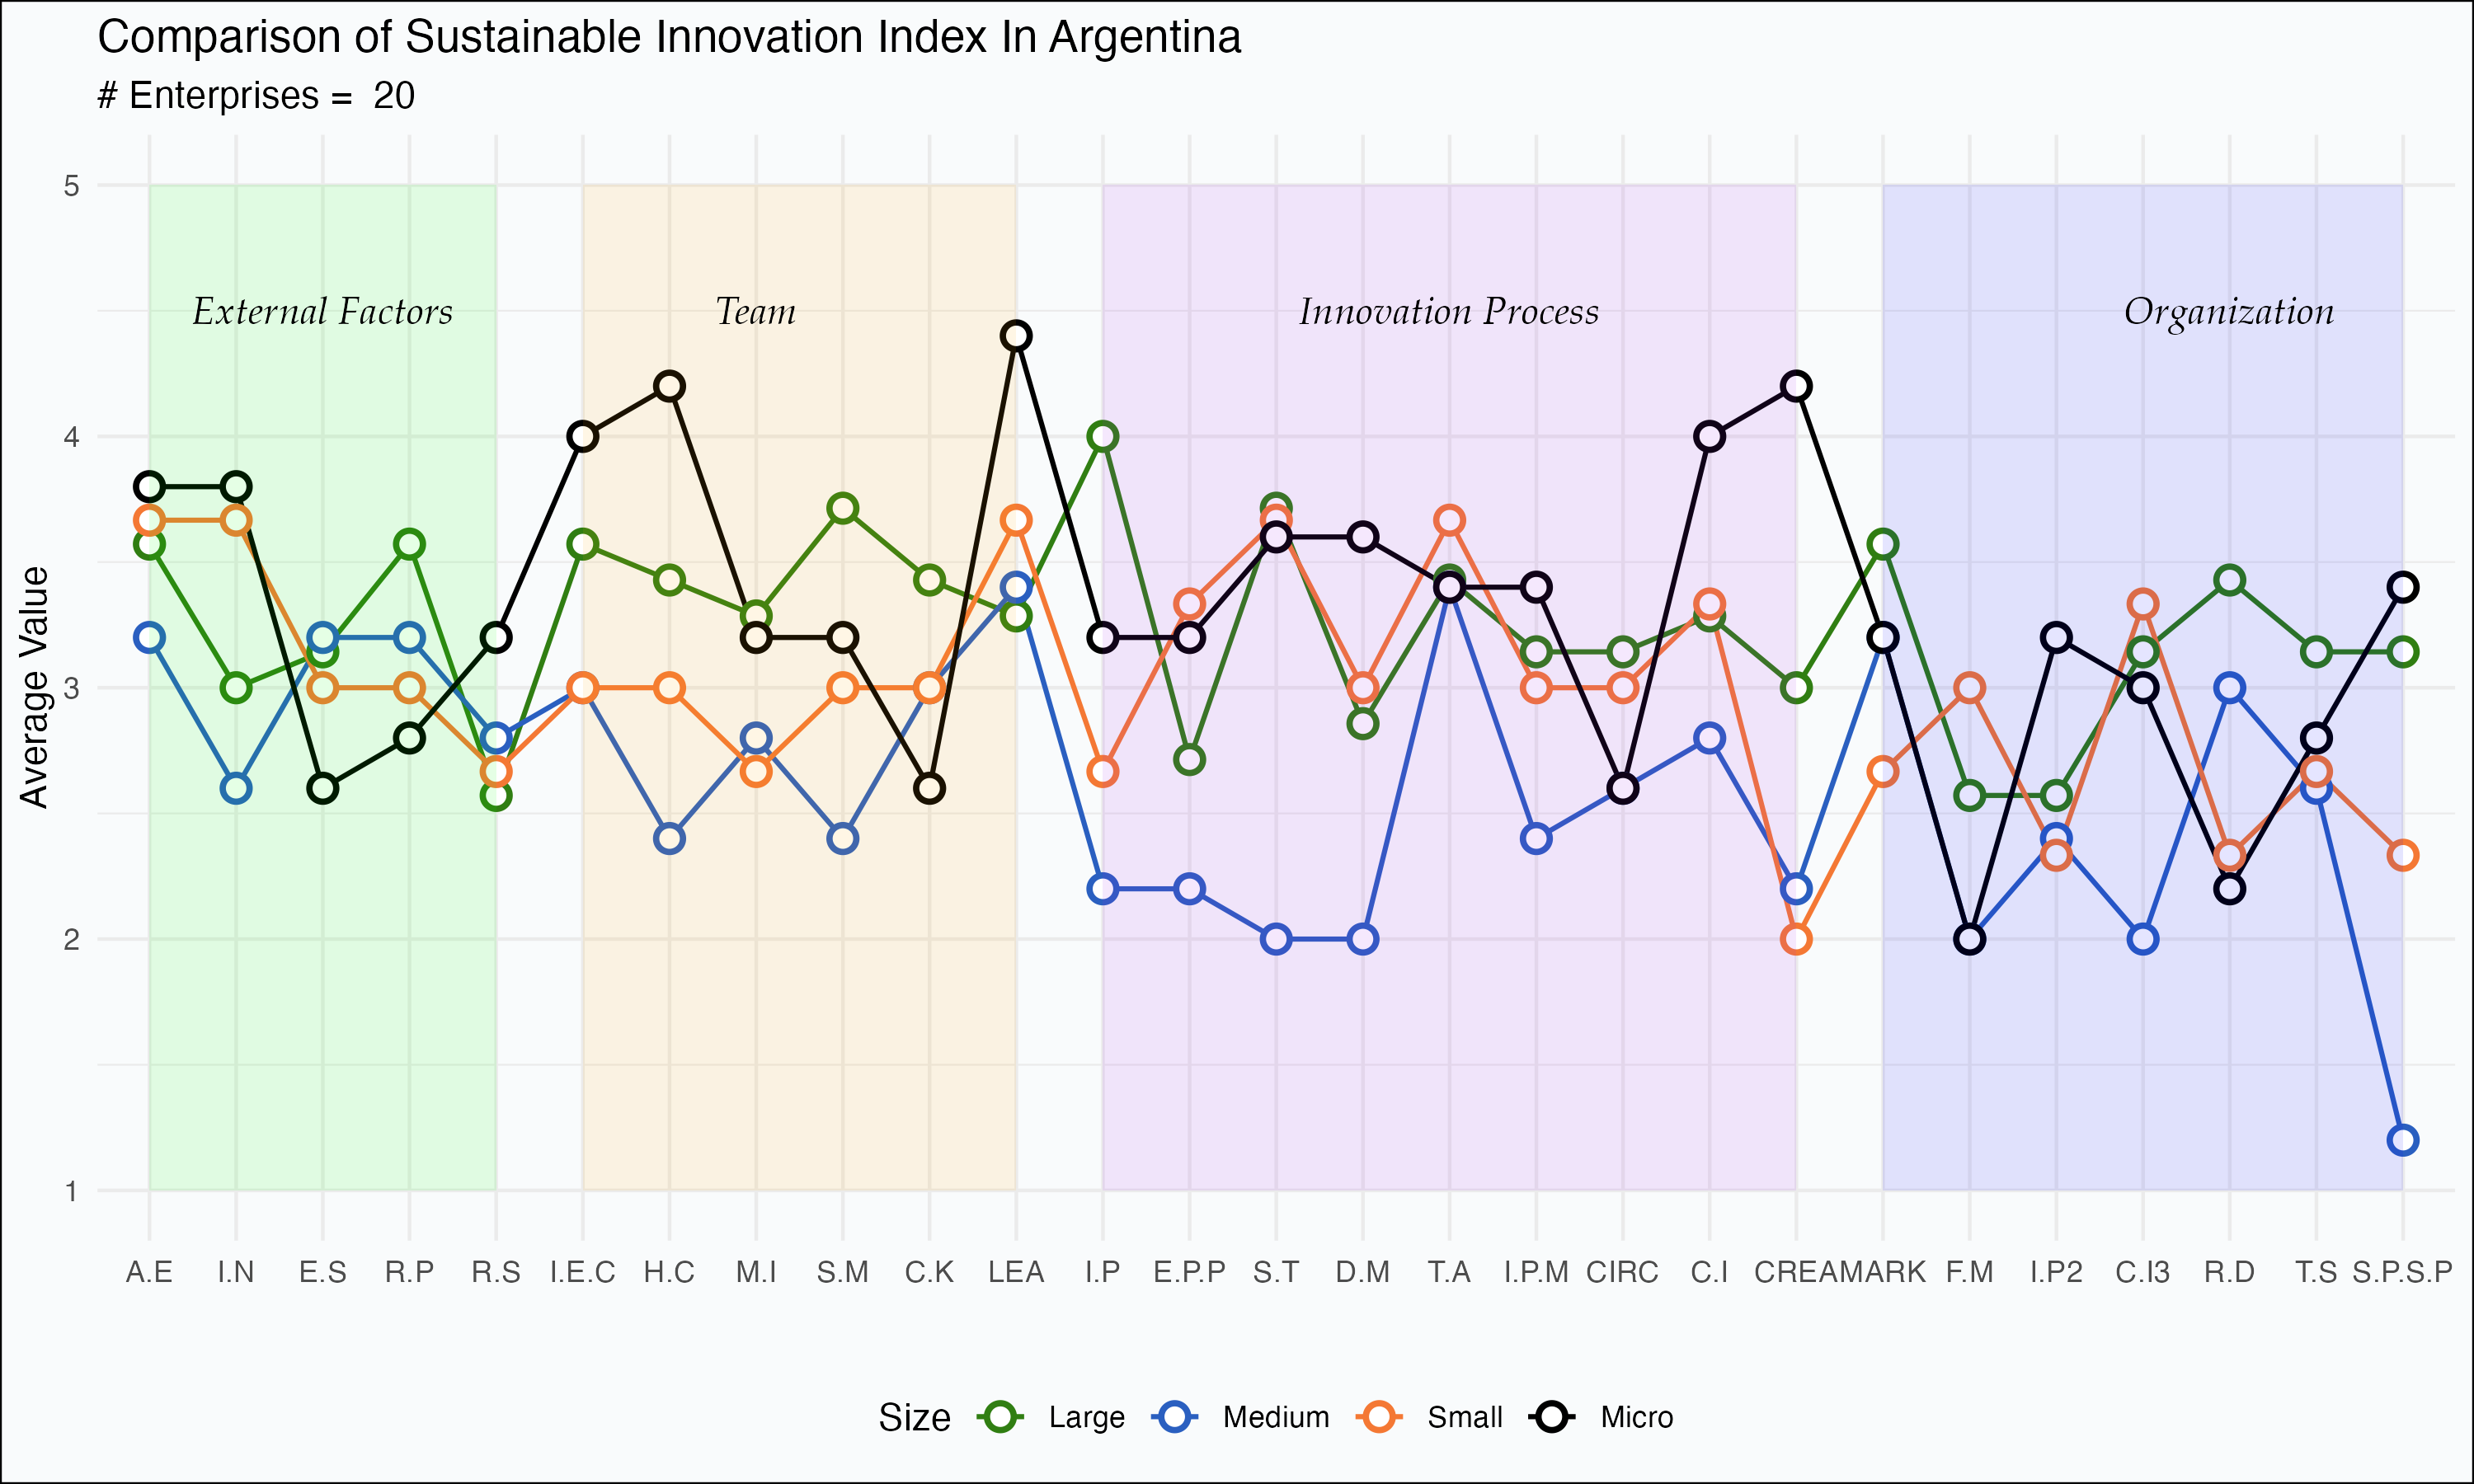
\includegraphics[width=0.9\linewidth,height=\textheight,keepaspectratio]{figures/1.3/Comparison-Argentina.png}

}

\caption{\label{fig-AR}Global Sustainable Innovation index per practice
at Argentina}

\end{figure}%

The analysis of Argentinian companies reveals distinct patterns in
sustainable innovation maturity across different firm sizes, as
summarized below.

Large enterprises (7 in total) demonstrate an intermediate to high level
of maturity (between 3.0 and 4.0). They perform particularly well in the
\emph{Team} and \emph{Innovation Process} practices, where results are
both solid and consistent. However, they show specific weaknesses in
\emph{External Supervision} (2.7), \emph{Financial Management}, and
\emph{Intellectual Property}, all with average scores below 3.0. These
findings indicate that large companies possess robust organizational
structures but still have room for improvement in external monitoring
and resource management.

On the other hand, medium-sized companies (5 in total) display a
medium-to-low maturity level (\textasciitilde{} 2.8), with homogeneous
evaluations and no major contrasts between factors. Their main strengths
are found in \emph{Leadership} (3.4) and \emph{Task Organization} (3.6),
whereas significant weaknesses appear in Organizational Management,
particularly \emph{Sustainable Purchasing within the Supply Chain}
(1.4). Overall, these companies exhibit a lack of comprehensive
coordination across their innovation processes.

\emph{Regarding the }small enterprises (3 in total) present low to
medium maturity levels (\textasciitilde{} 2.8), with strengths in
\emph{Analysis of the Environment and Innovation Networks (above 3.7)
}and* leadership \emph{(LEA 3.6), but with heterogeneous Innovation
Processes where weaknesses are evident in }Creativity \emph{(2.0) and
}Innovation Portfolio* (2.7), and \emph{limited organizational
management}, with exceptions such as \emph{Continuous Improvement}
(3.3).

Micro-enterprises (5 in total) exhibit a more dispersed maturity
profile. They perform well in external factors, including Environmental
Analysis and Innovation Networks (both near 4.0), and in team-related
dimensions such as Internal and External Communication, Human Capital,
and Leadership, all scoring above 4.0. Additionally, they show promising
results in Creativity (4.2) and Continuous Improvement (4.0). However,
these strengths are counterbalanced by structural weaknesses in
Financial Management (2.0), R\&D (2.2), and Knowledge Capitalization
(2.6), which hinder the consolidation of their innovation capabilities.

Overall, the variation in performance among Argentinian companies is not
strongly correlated with firm size. This uniformity may be influenced by
the regional industrial ecosystem, where local institutional support and
development programs contribute to a more level playing field among
companies.

In general terms, practices associated with operational management tend
to achieve higher evaluations than those linked to strategic planning,
which explains the lower average scores in the Organizational Pillar.

\subsection{Chile}\label{chile}

In the case of Chile in Figure~\ref{fig-CH}, analysis of the level of
maturity in innovation and business management shows notable differences
between companies of different sizes, although the results should be
interpreted with caution due to the limited sample size.

\begin{figure}[H]

\centering{

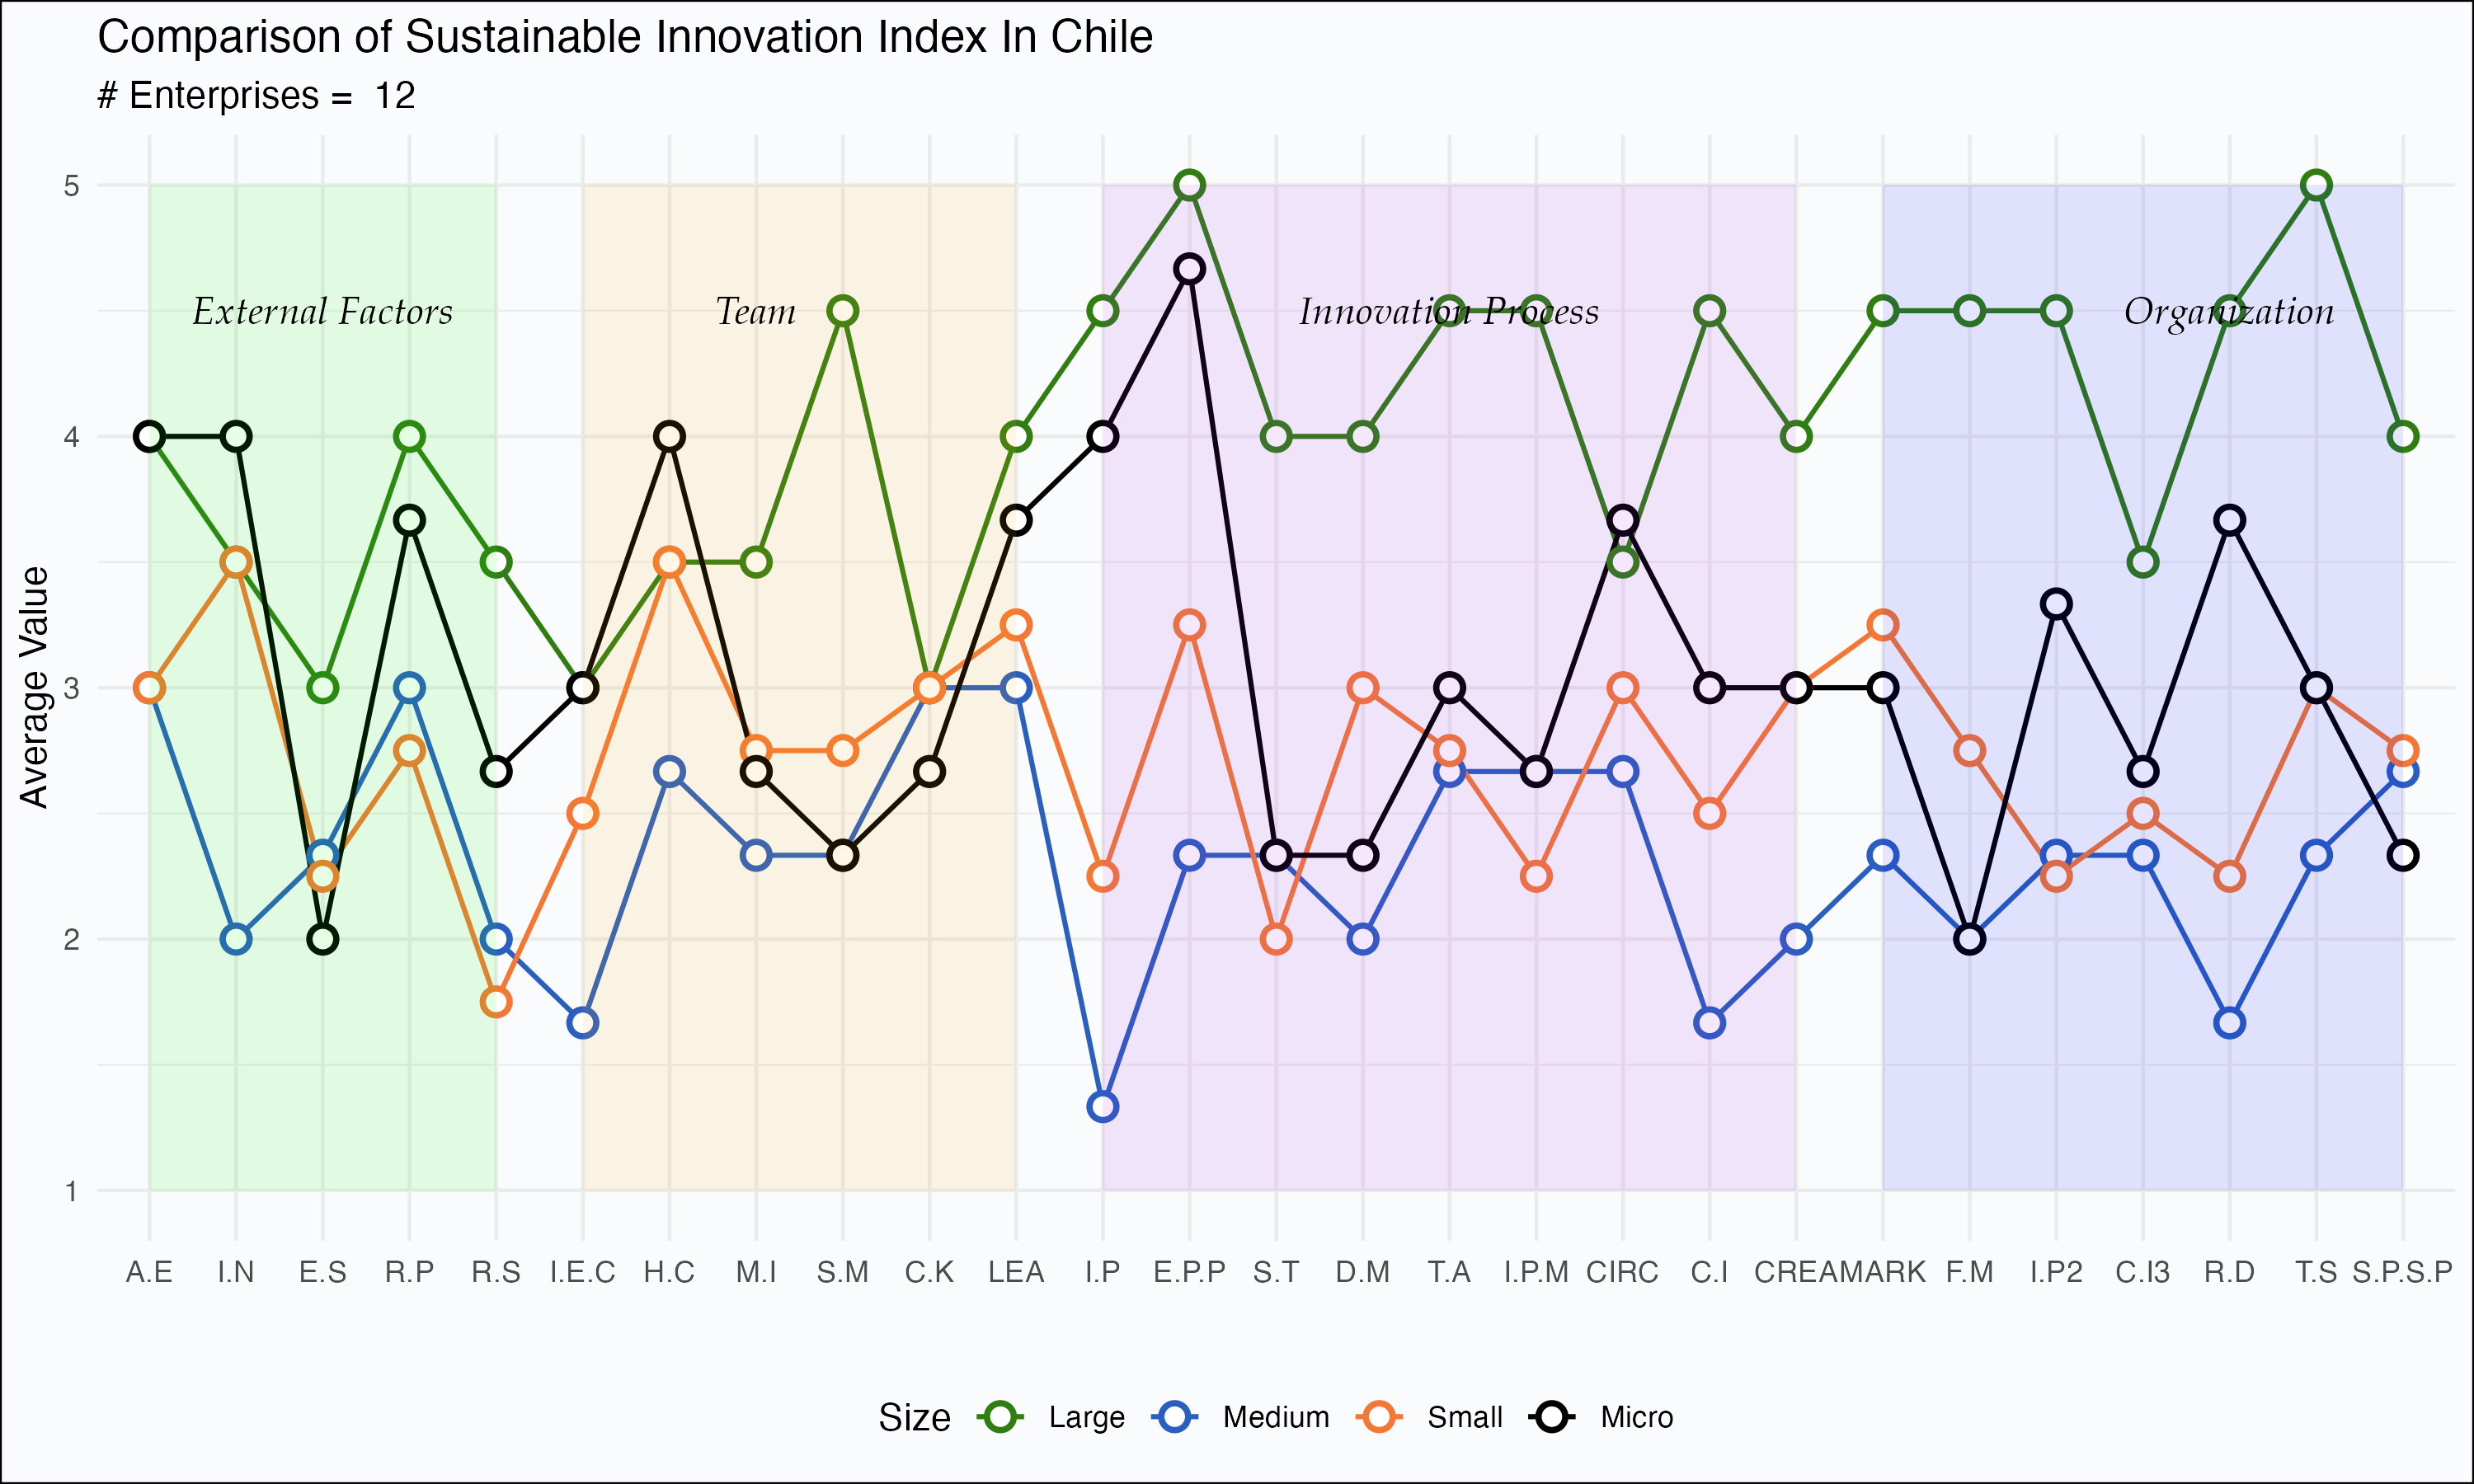
\includegraphics[width=0.9\linewidth,height=\textheight,keepaspectratio]{figures/1.3/Comparison-Chile.png}

}

\caption{\label{fig-CH}Global Sustainable Innovation index per practice
at Chile}

\end{figure}%

Large companies (two in total) have the highest levels of maturity, with
scores between 4 and 5 in most pillars, standing out in Innovation
Process (with \emph{Eco-innovation in products and processes} at 5 and
\emph{Technological Strategy}, \emph{Task Organization},
\emph{Innovation Project Management}, and \emph{Customer Integration} at
4.5) and in Organization, where the \emph{Marketing, Financial
Management, Intellectual Property}, and \emph{Research and Development
}factors reach averages of 4.5 and \emph{Technological Strategy} reaches
5. They also excel in Team, with high values in \emph{Skills Management}
(4.5) and \emph{Leadership} (4.0), and consistent performance in
external factors, with averages between 3 and 4, indicating an advanced
level of internal structuring and management.

In contrast, medium, small, and micro companies show intermediate or low
levels of maturity, with overall averages between 2 and 3, evidencing
processes in consolidation and heterogeneity in results. Medium-sized
companies generally have the lowest assessment profile, showing
weaknesses in the innovation process (\emph{Innovation Portfolio} 1.3,
\emph{Eco-innovation in products and processes} 2.3) and organizational
management (\emph{Research and Development} 1.7, \emph{Financial
Management} 2.0). Small companies obtain averages close to 2.5, with
better results in Innovation \emph{Networks} (3.5) and \emph{Leadership}
(3.5), but with low values in \emph{Regulatory Support} (1.6) and basic
innovation processes (\emph{Innovation Portfolio, Support Tools,
Innovation Project Management} \textasciitilde2). Finally,
micro-enterprises combine strengths in \emph{Eco-innovation in Products
and Processes }(4.7), \emph{Environment Analysis and Innovation Networks
}(4.0), and \emph{Human Capital} (4.0) with weaknesses in \emph{External
Supervision} (2.0) and \emph{Financial Management} (2.0), suggesting
partial and uneven maturity.

The Chilean context shows a heterogeneous business profile, where
leadership, planning, and technological process capabilities are
concentrated in a small group of companies, while the rest of the
business fabric maintains less mature structures with potential for
strengthening.

These results, although based on a limited sample, indicate the need to
continue promoting the systematization of innovative practices,
knowledge management, and inter-company coordination as key areas for
advancing toward greater levels of maturity and competitiveness in the
Chilean business environment.

\section{Analysis of the Sustainable Innovation Index by Size of the
Enterprise}\label{analysis-of-the-sustainable-innovation-index-by-size-of-the-enterprise}

\subsection{Large companies at Colombia,
Argentine,Chile}\label{large-companies-at-colombia-argentinechile}

This section presents the comparative Analysis of the Innovation Index
for large enterprises across Colombia, Argentine, and Chile.\\
Figure~\ref{fig-large} shows the assessment of factors for large size
companies in the Colombian, Argentinian and Chilean context. In total,
20 enterprises were considered in the set of answers. From the results
is observed that large Chilean companies stand out as the best rated in
indicators associated with innovation processes and organizational
management, with average values in the range of 4-5. However, it should
be noted that the number of companies evaluated in Chile was lower
compared to those in Colombia and Argentina.

\begin{figure}[H]

\centering{

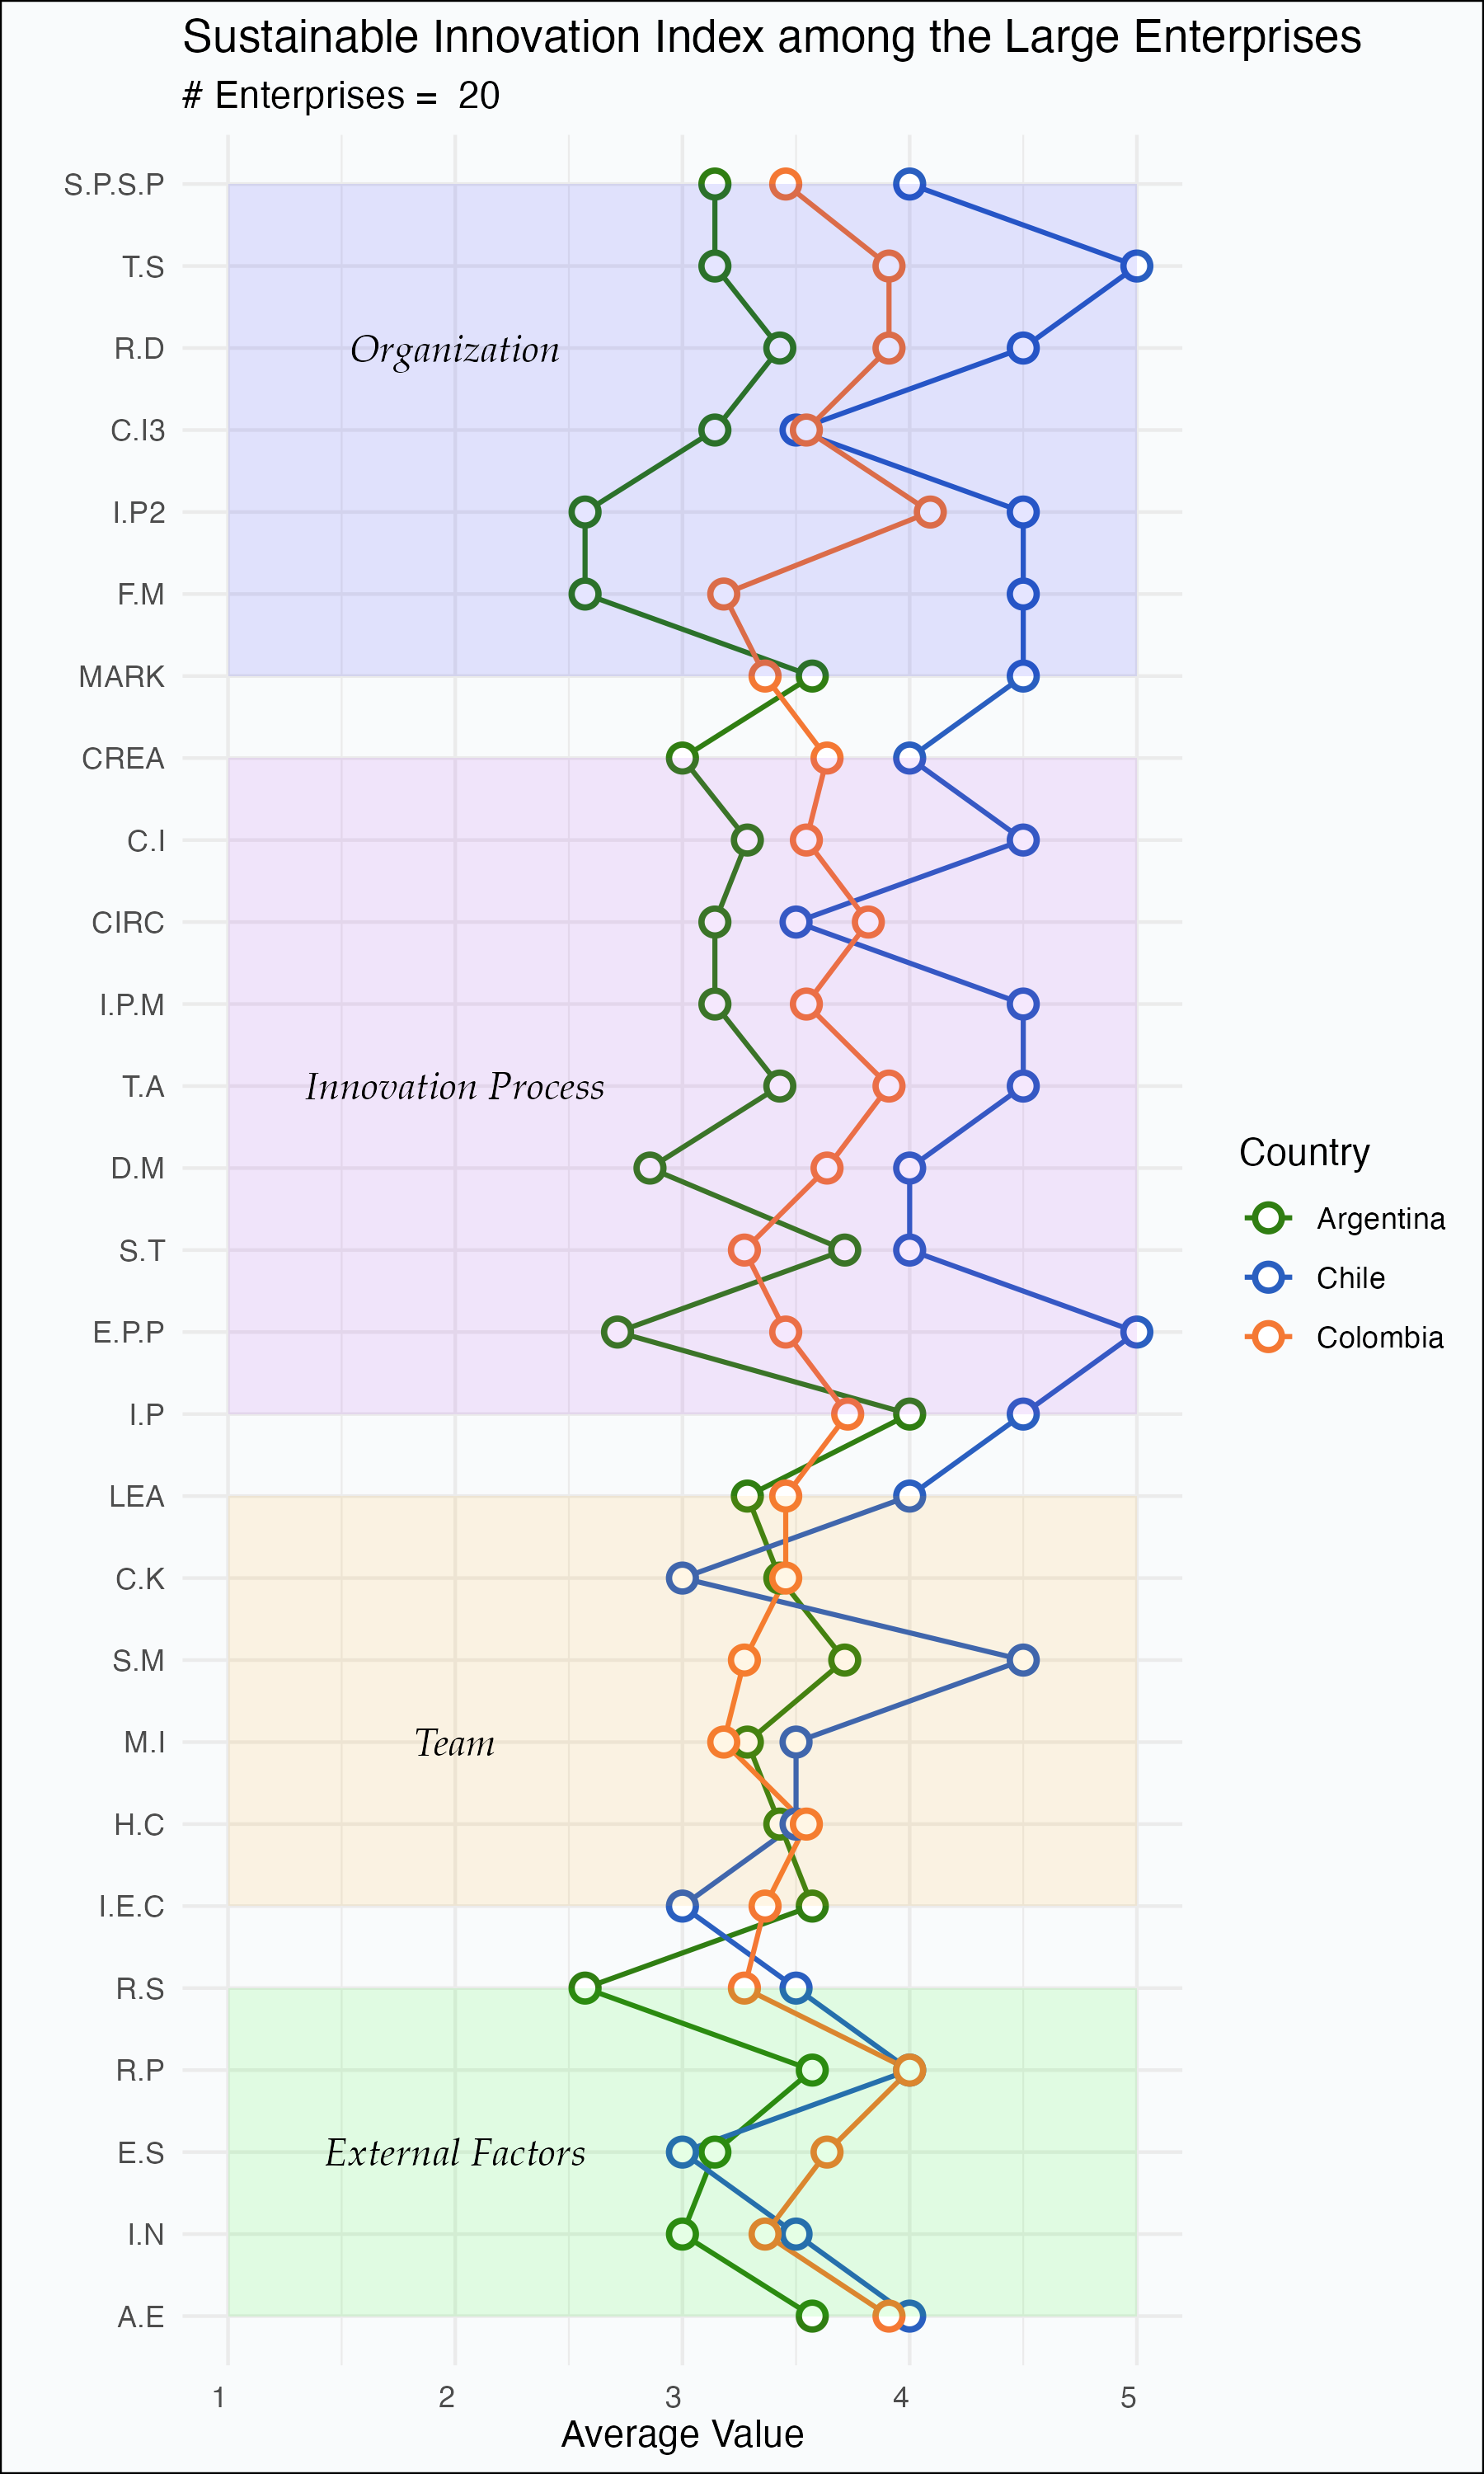
\includegraphics[width=0.6\linewidth,height=\textheight,keepaspectratio]{figures/1.3/Comparison-Large.png}

}

\caption{\label{fig-large}Comparison of the practices for Large
companies Argentina, Colombia and Chile}

\end{figure}%

Large Colombian companies, on the other hand, show intermediate levels
of maturity in these factors (averages in the range of 3.4), while large
Argentine companies receive the lowest ratings, with average values
between 2.5 to 3.5. These results show that large Chilean companies have
internalized and consolidated innovation processes and tools within the
organization, which is supported internally by clear organizational
management in areas relevant to innovation processes, such as
\emph{research and development, intellectual property management,
financial management}, and \emph{marketing}.

In the case of Colombia, the results of large Colombian companies show
\emph{innovation} and \emph{organizational management processes and
practices} in the process of maturing to carry out sustainable
innovations, with balanced levels of maturity in their practices.
Finally, the values reported by large Argentine companies show
medium-low levels of maturity in terms of innovation and organizational
processes, which must be strengthened for the development of sustainable
innovations.

Regarding practices associated with team management and external
factors, Figure~\ref{fig-large} shows similar behavior in large
companies in the three countries, except for the factors such as,
\emph{Skill Management (S.M)} and \emph{Regulatory Support (R.S)}. In
the case of S.M, large Chilean companies report high maturity values
(average 4.5), while large Colombian and Argentine companies report
intermediate maturity values close to 3.5. Therefore, large Chilean
companies would have skill management strategies more aligned with
innovation and sustainability than large Colombian and Argentine
companies. However, large Colombian and Argentine companies show a high
level of maturity in this practice.

Finally, in relation to regulatory support, large Argentine companies
report having low regulatory support compared to Chilean and Colombian
companies. In other words, they report having few government policies
and programs to support the development of sustainable innovations.
Despite this, large companies are trying to take advantage of
opportunities for \emph{innovation} (A.E high) and \emph{collaboration}
(I.N medium-high).

\subsection{Medium companies at Colombia,
Argentine,Chile}\label{medium-companies-at-colombia-argentinechile}

Figure~\ref{fig-medium} shows the assessment of factors for medium size
companies in the Colombian, Argentinian and Chilean context. In total,
20 enterprises were considered in the set of answers.

\begin{figure}[H]

\centering{

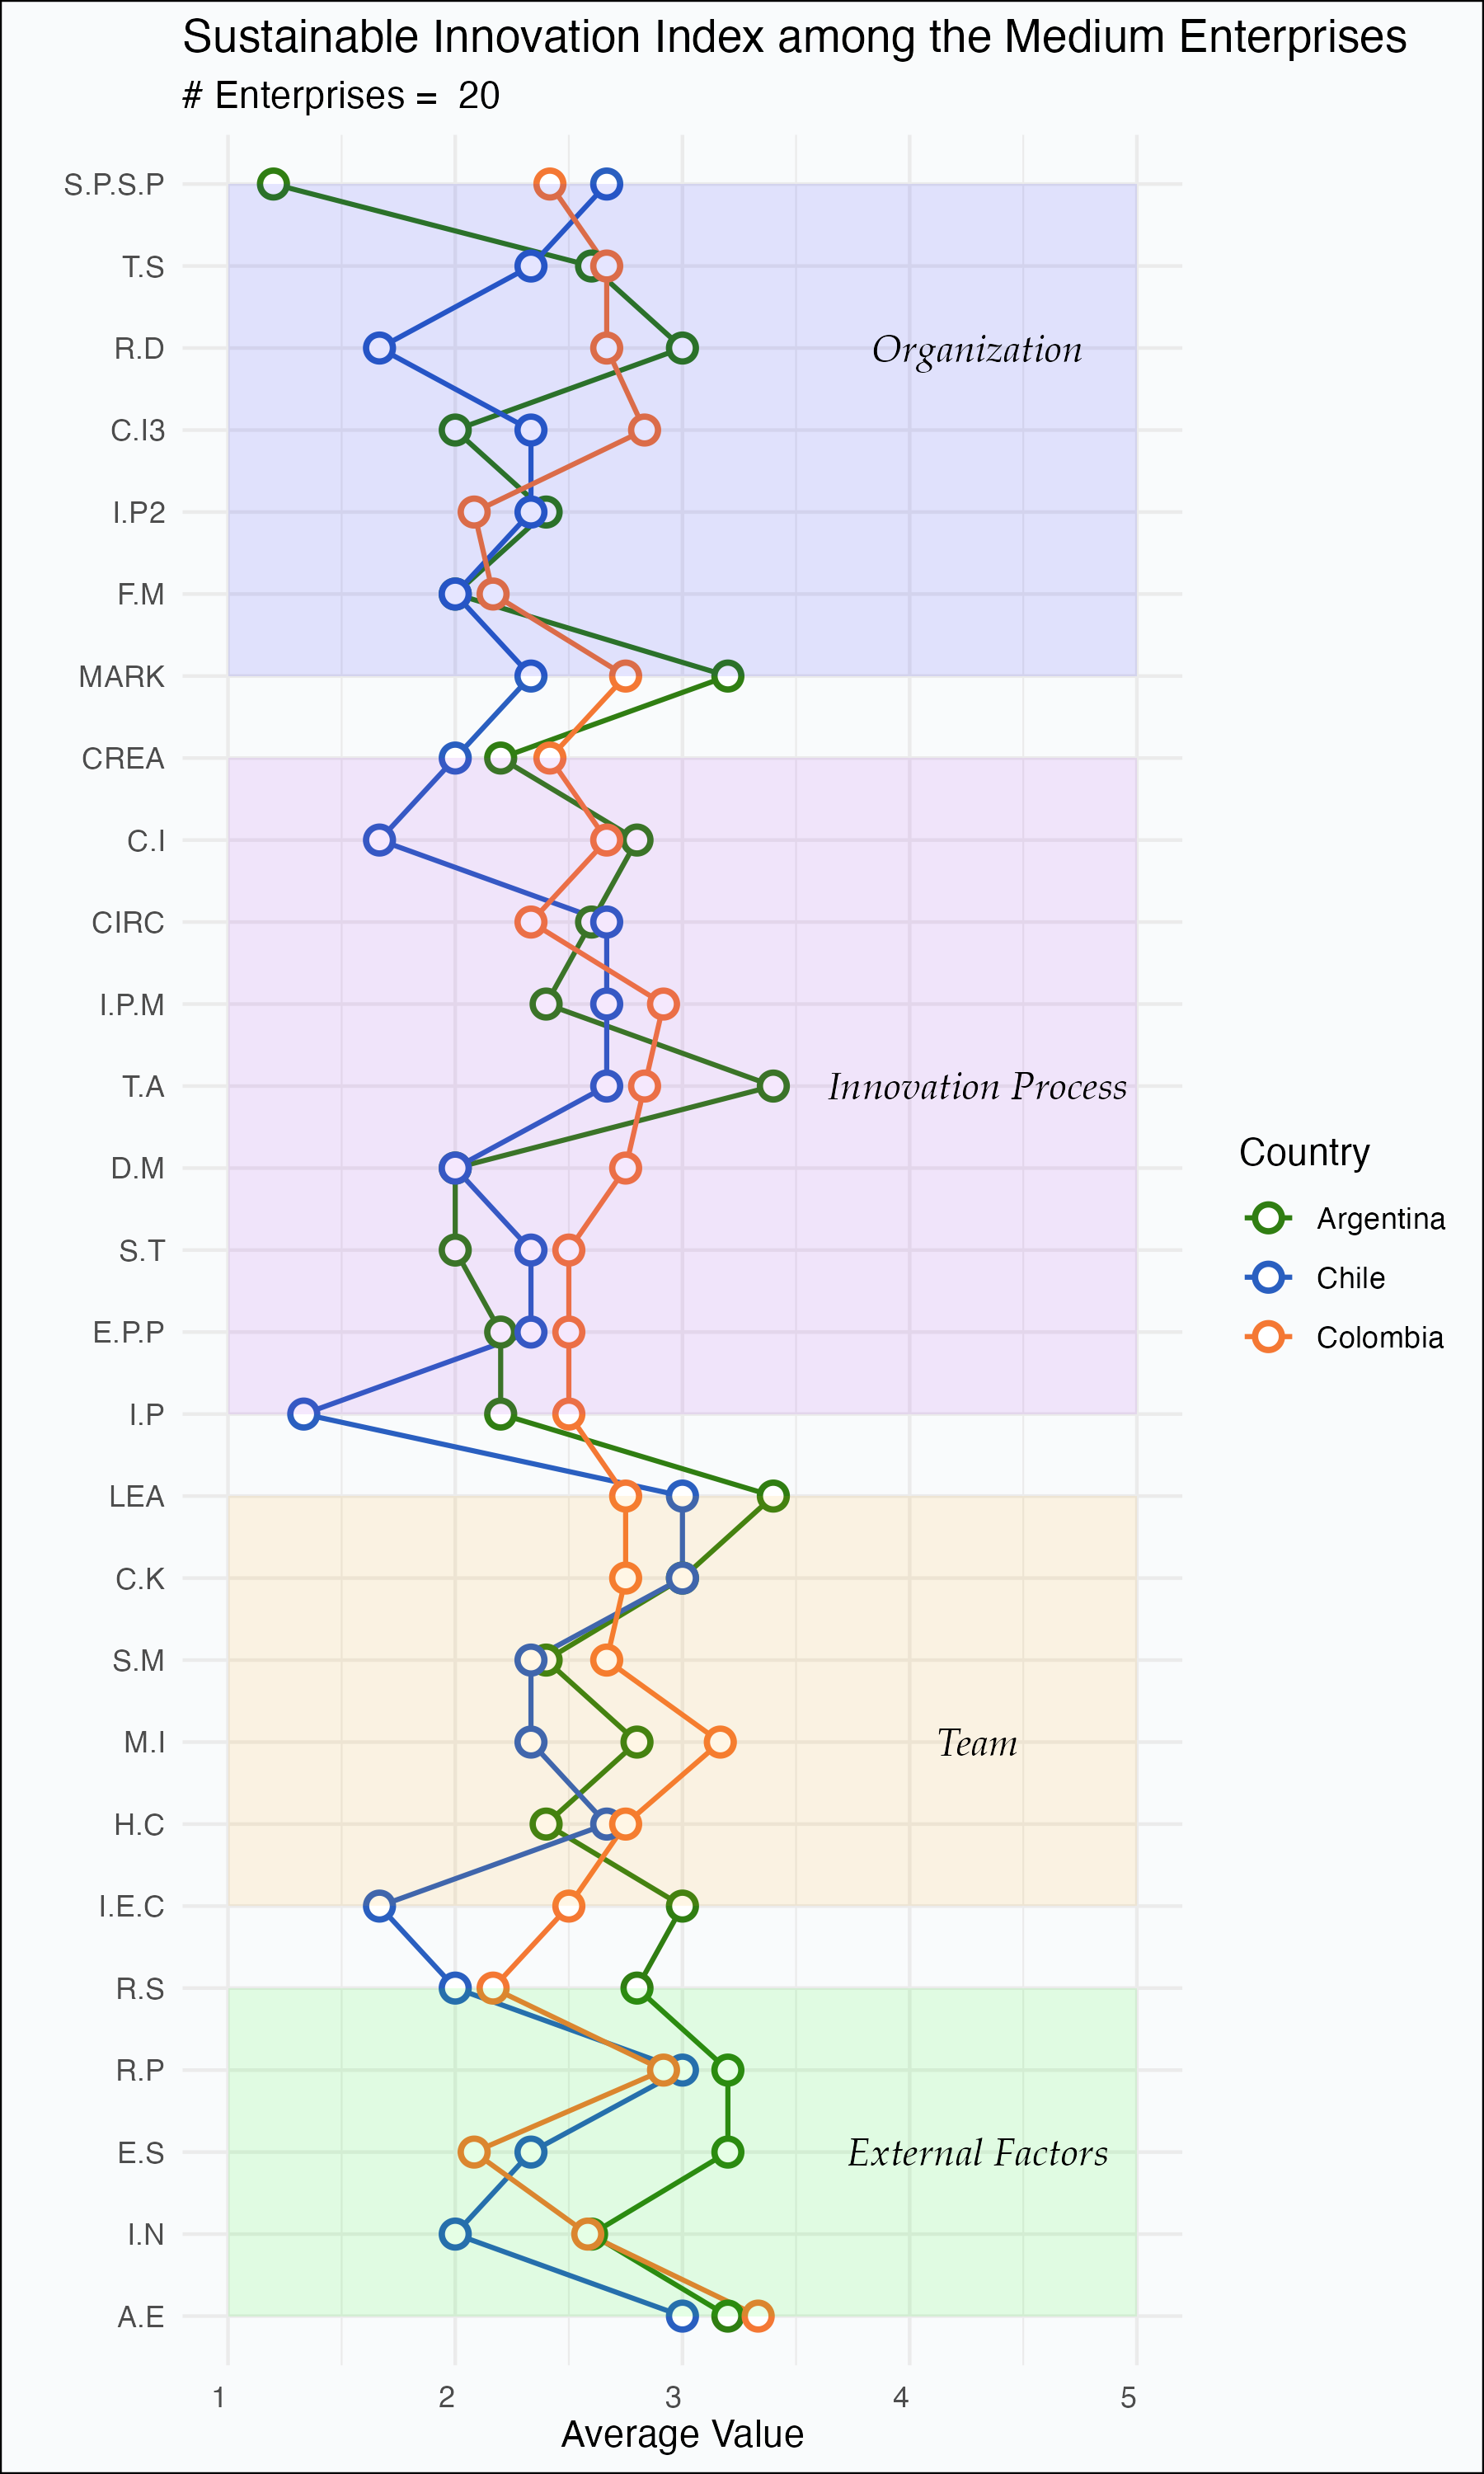
\includegraphics[width=0.6\linewidth,height=\textheight,keepaspectratio]{figures/1.3/Comparison-Medium.png}

}

\caption{\label{fig-medium}Comparison of the practices for Medium
companies}

\end{figure}%

Medium-sized companies in Colombia, Argentina, and Chile show
low-to-medium levels of maturity in the factors evaluated, with average
values equal to or below 3.5.

In the case of factors associated with \textbf{Organizational
management}, the lowest factors in the three countries correspond to
\emph{intellectual property management (IP2) }and \emph{financial
management (F.M)}, which represent the greatest challenges in this area
for medium-sized companies in the three countries. In the particular
case of Chile, \emph{research and development (R\&D)} is added as an
additional management need. In the case of Argentina, procurement
management with a focus on \emph{sustainability (S.P.S.P)}.

In relation to \textbf{Innovation processes}, low levels of development
can be observed in terms of innovation strategies, processes, and tools
to support the development of sustainable innovations in medium-sized
companies. In particular, Chilean and Argentine medium-sized companies
have lower values compared with Colombian counterparts, with the lowest
values being those associated with the \emph{development of
methodologies (D.M), sport tools (S.T)}, and \emph{eco-innovation in
products and processes}, thus representing the greatest needs of this
group of companies to enhance their capacity for sustainable innovation.

Considering the factors associated with \textbf{Team management}, these
show similar maturity results in medium-sized companies in the three
countries, although \emph{skills management and motivation to innovate}
emerge as the two lowest-performing practices.

Finally, in relation to the values associated with \textbf{External
Factors}, it is worth mentioning that companies try to take advantage of
opportunities in the \emph{environment (A.E.)} through collaboration
\emph{(I.N.)}. However, the regulatory environment (\emph{E.S., RP},
medium-low) and government incentives (low \emph{R.S}) are not mature
enough to promote the development of sustainable innovations.

\subsection{Small companies at Colombia,
Argentine,Chile}\label{small-companies-at-colombia-argentinechile}

Regarding the small companies in total 13 enterprises were considered in
the set of answers (Figure~\ref{fig-small}). Small Colombian companies
report low-to-medium levels of maturity in most practices compared to
Argentina and Chile. In other words, small Colombian companies face
difficulties in terms of organizational management, formalization and
support for innovation processes, team management, and an adequate
context for taking advantage of opportunities to carry out sustainable
innovations.

\begin{figure}[H]

\centering{

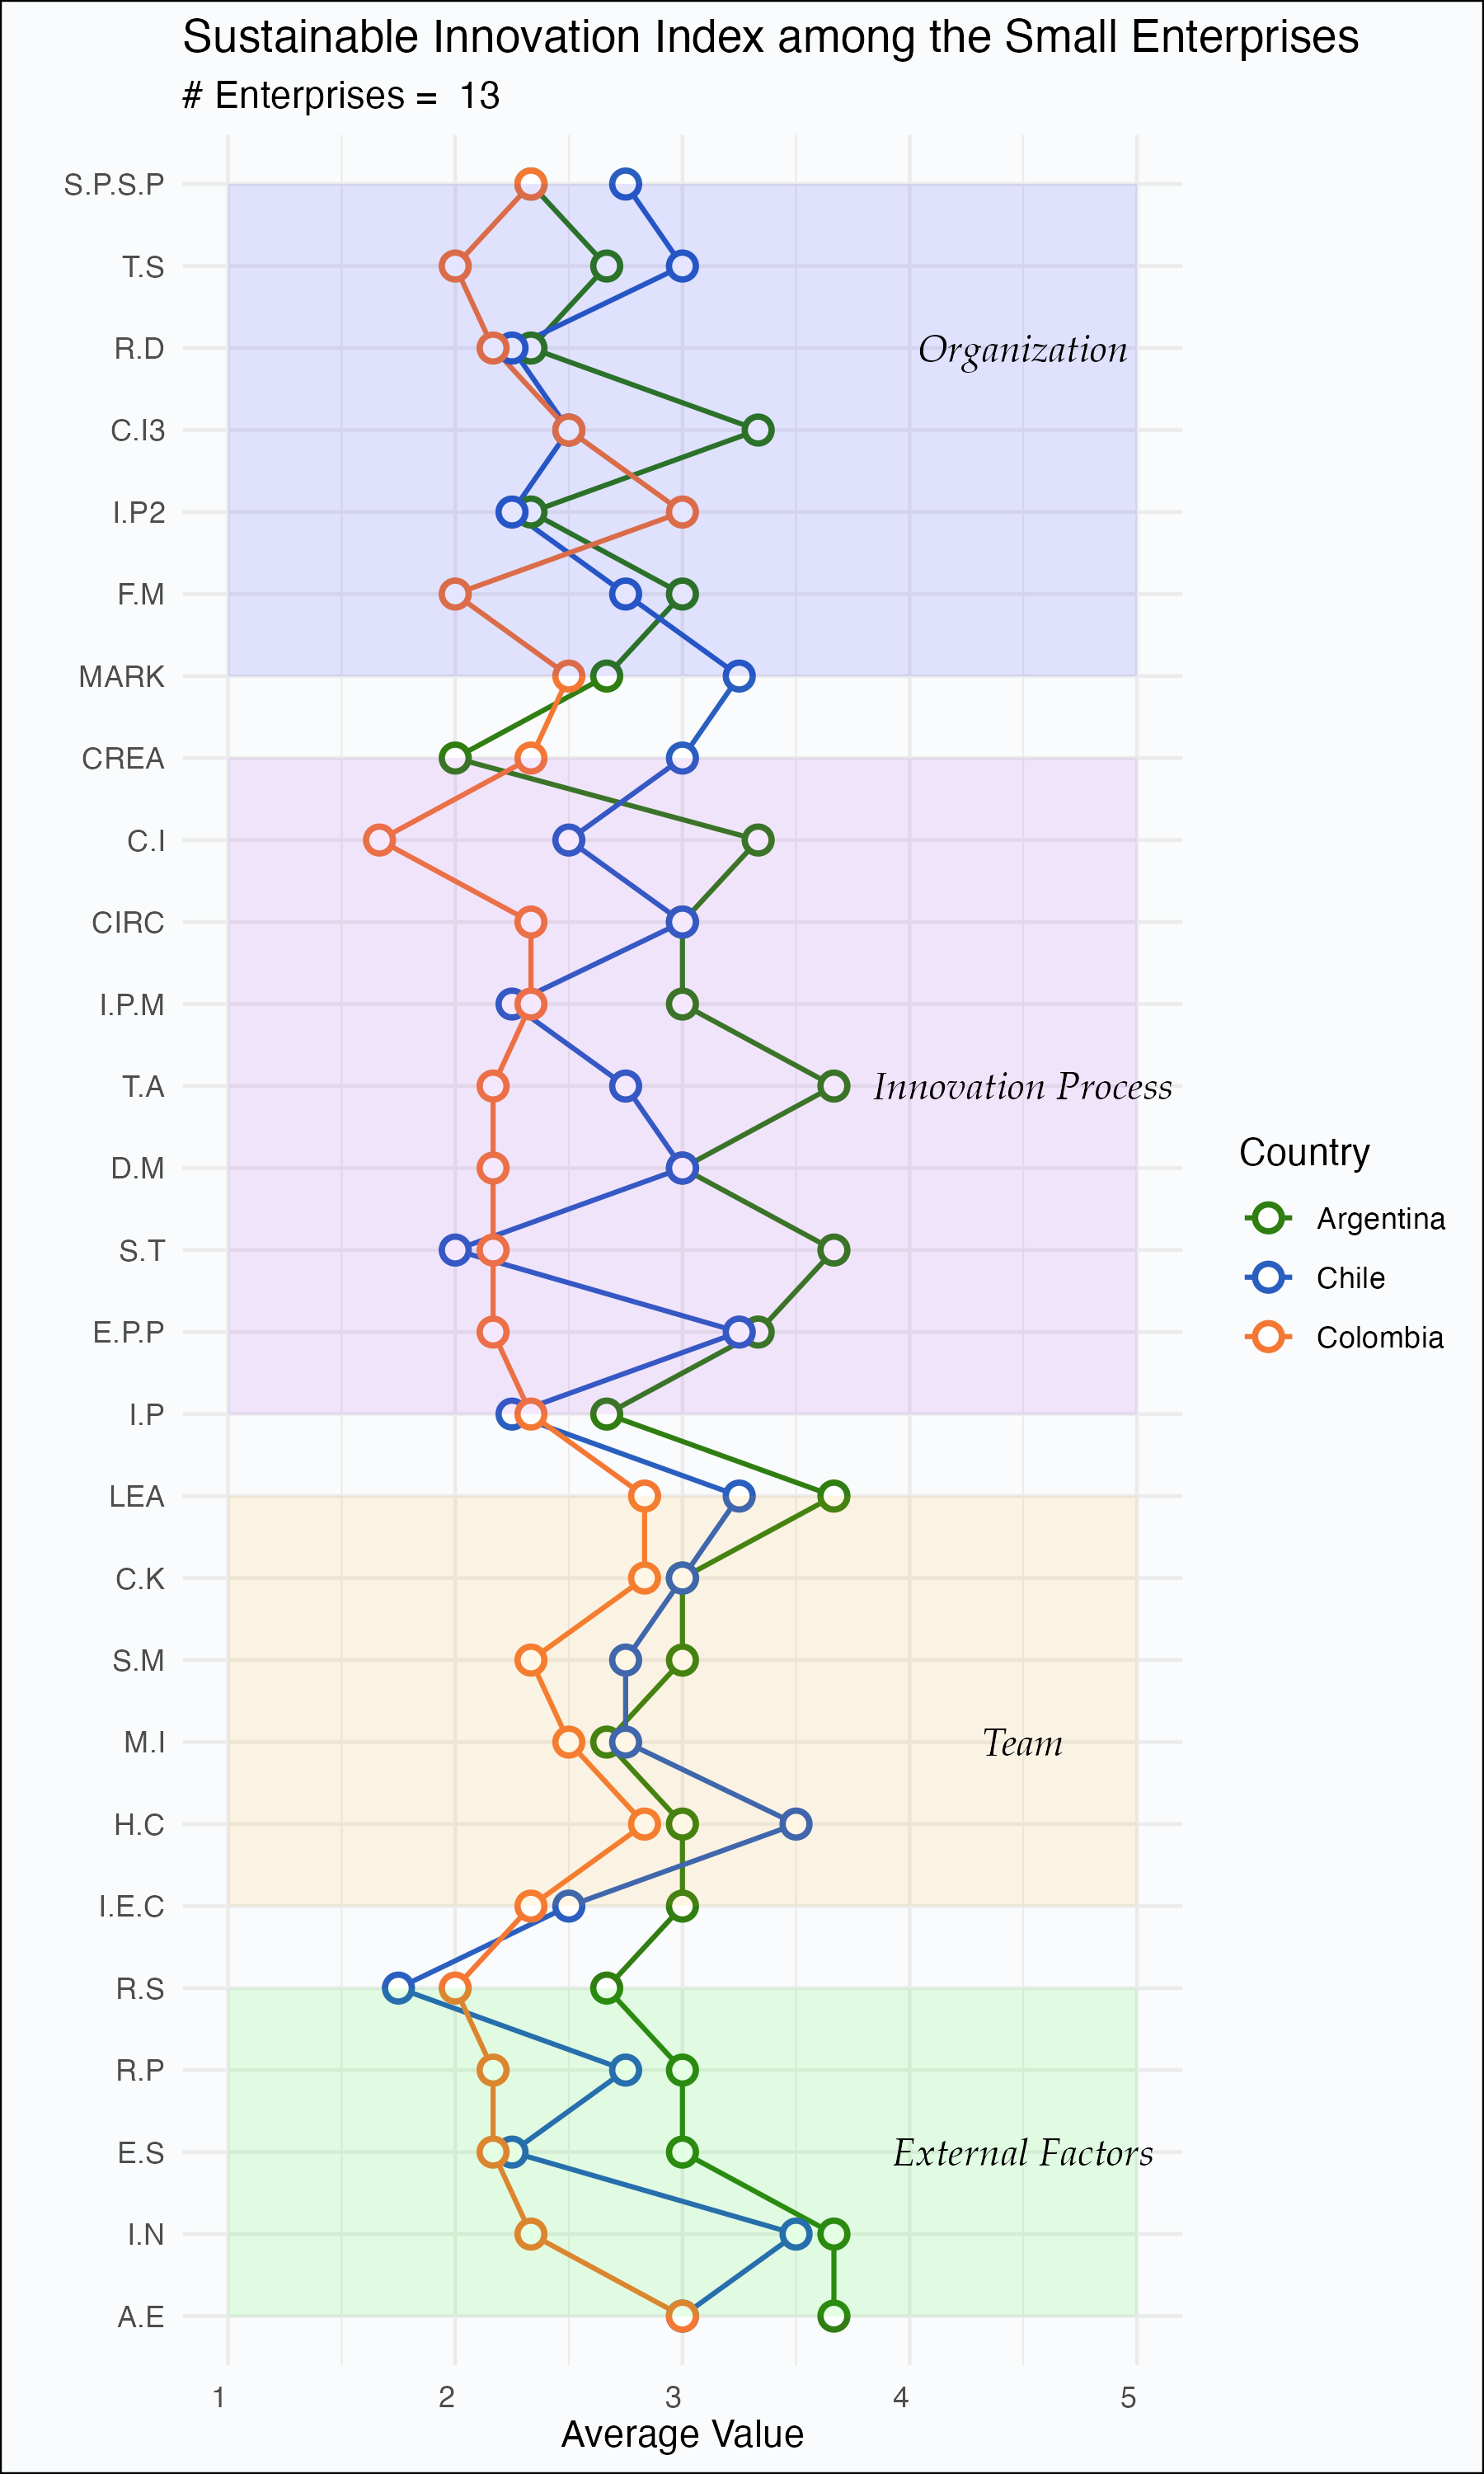
\includegraphics[width=0.6\linewidth,height=\textheight,keepaspectratio]{figures/1.3/Comparison-Small.png}

}

\caption{\label{fig-small}Comparison of the practices for Small
companies}

\end{figure}%

For their part, Argentina and Chile show better, but not greatly
superior, levels of maturity. In particular, small Argentine companies
show better levels in all four categories, representing better
conditions (especially contextual and at the level of innovation
processes) for carrying out sustainable innovations compared to Chile
and Colombia.

\subsection{Micro companies at Colombia,
Argentine,Chile}\label{micro-companies-at-colombia-argentinechile}

Within the micro size companies in the Colombian, Argentinian and
Chilean context 15 enterprises were considered, Figure~\ref{fig-micro}
present the results obtained.

\begin{figure}[H]

\centering{

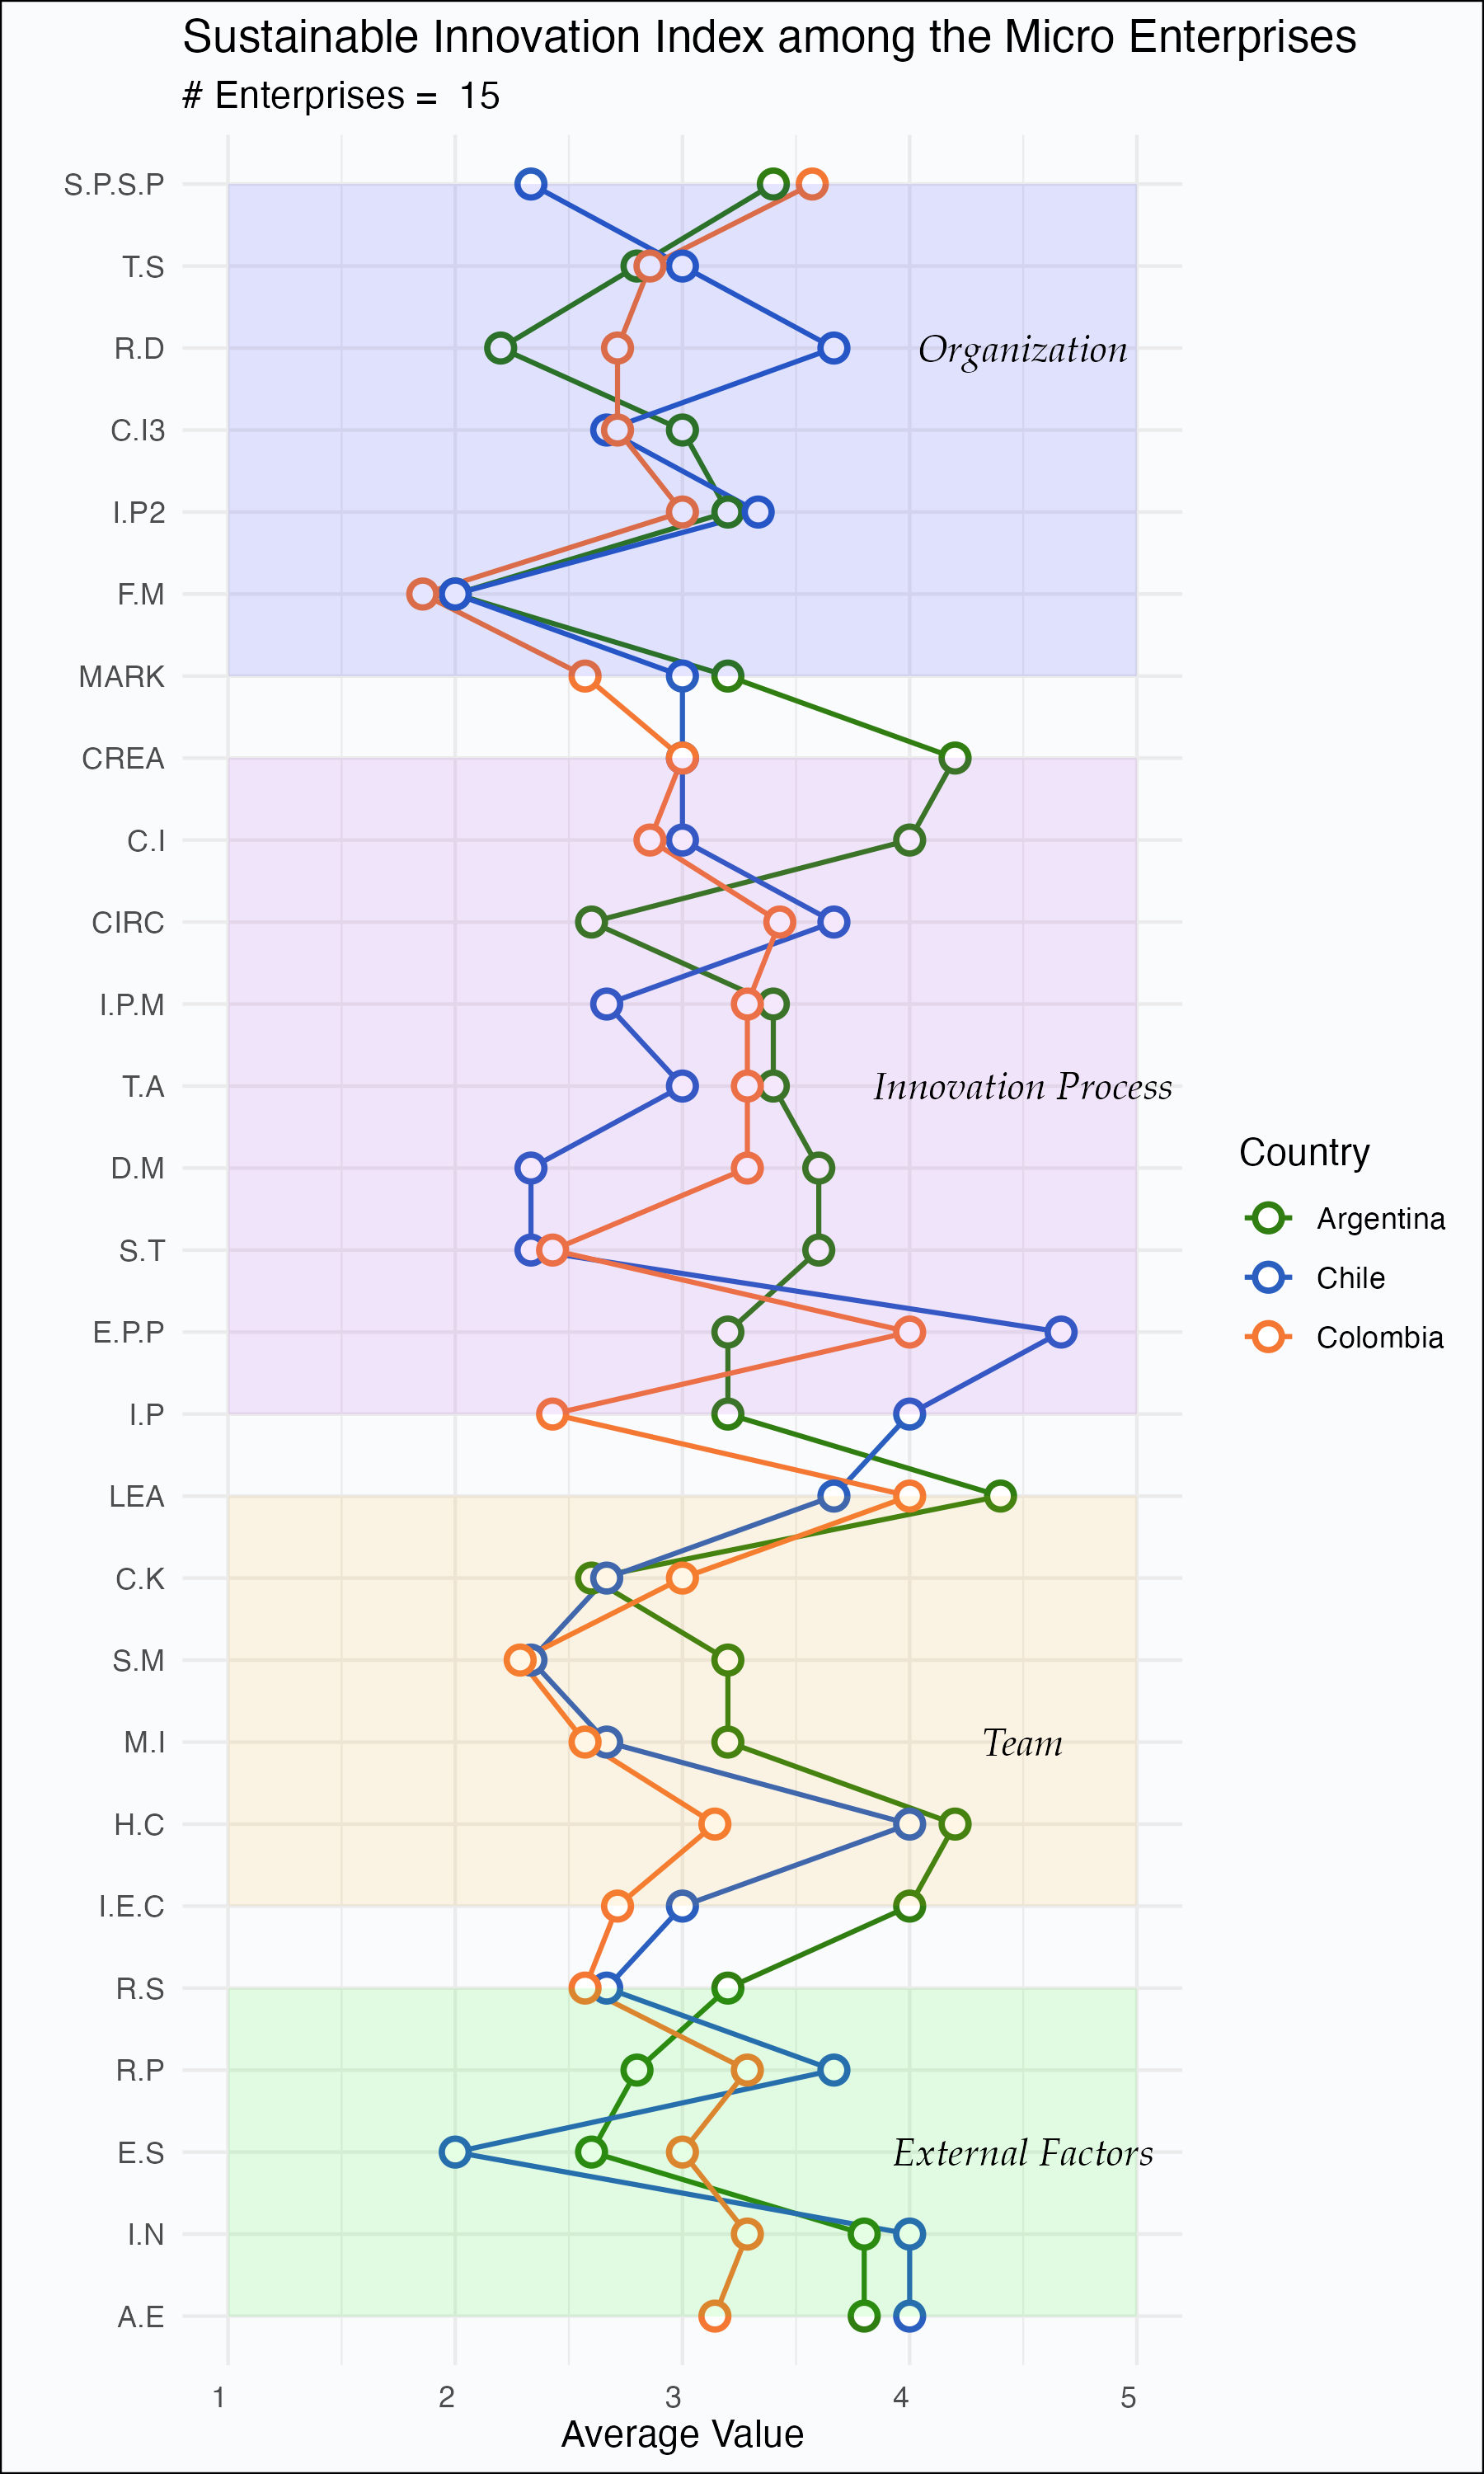
\includegraphics[width=0.6\linewidth,height=\textheight,keepaspectratio]{figures/1.3/Comparison-Micro.png}

}

\caption{\label{fig-micro}Comparison of the practices for micro
companies}

\end{figure}%

In general, Colombian, Chilean, and Argentine microenterprises show
heterogeneous behavior in terms of their level of maturity in each
practice.

At the organizational level, microenterprises in all three countries
have needs in relation to financial management, with acceptable levels
of maturity (medium-high) in relation to the other practices in this
group. In terms of innovation processes, Argentine microenterprises seem
to have the most consolidated innovation processes and tools when
comparing the three countries, especially in r\emph{elation to
creativity, customer integration, design methodologies, and support
tools}. In terms of team management, micro-enterprises in the three
countries exhibit similar behaviors, although Argentine
micro-enterprises score higher \emph{in motivation to innovate} and
\emph{skills management}. \emph{Human capital management} and
\emph{leadership} excel as the highest-rated practices in this category.
Finally, in terms of environment and context, micro-enterprises in the
three countries report medium-high levels of maturity, indicating a
moderately favorable environment for sustainable innovation.

\section{Closure of WP1 of
TechTraPlastiCE}\label{closure-of-wp1-of-techtraplastice}

The present deliverable closure the Work Package 1 (WP1) of the
TechTraPlastiCE project. As stated in description of action, this WP
aimed to define instruments, create capacities and guide Universities in
identifying and understanding key barriers and leverage points of the
local plastic companies to encourage collaboration opportunities with
industries in each participating partner institution. After navigating
through this WP, universities will identify the most appropriate
industries and sectors to engage in the later stages of the projects,
identifying fundamental driving forces for innovation as illustrated in
Figure~\ref{fig-baseline}.

\begin{figure}[H]

\centering{

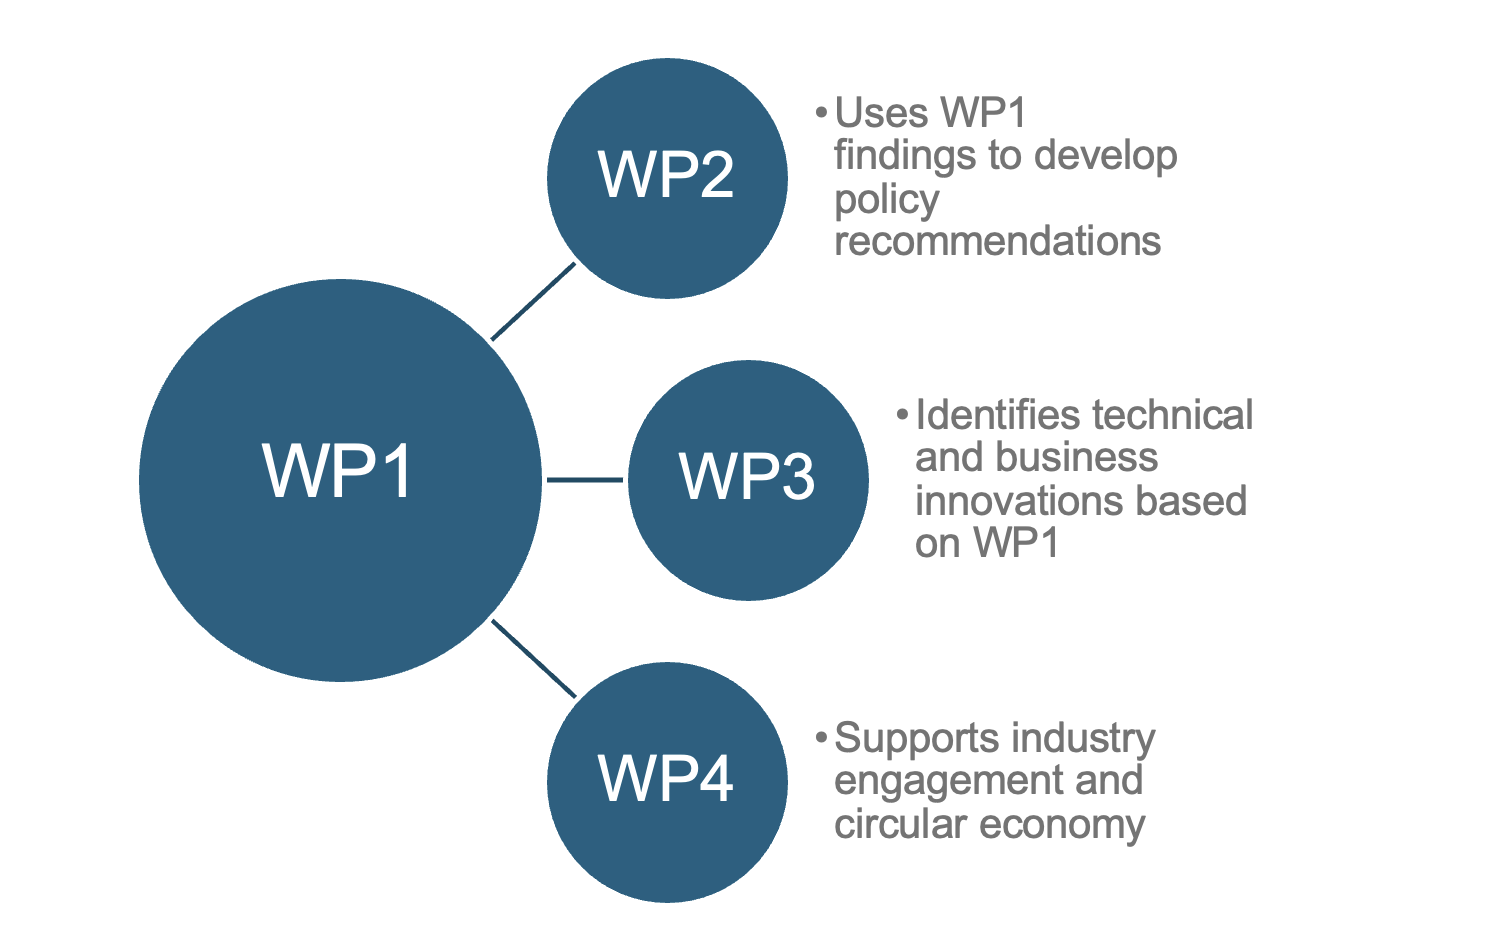
\includegraphics[width=0.7\linewidth,height=\textheight,keepaspectratio]{figures/1.1/Fig1.png}

}

\caption{\label{fig-baseline}WP1 baseline for TechTraplastiCE Project}

\end{figure}%

The deliverable 1.1 of WP1 under the TechTraPlastiCE project establishes
a comparative framework to understand the barriers and benefits of
applying local plastics legislation in Argentina, Chile, and Colombia.
Its main objective is to provide a shared baseline for analyzing
regulatory structures, institutional gaps, and key stakeholders across
the plastic value chain, supporting the transition toward a circular
economy in Latin America.

The framework was developed collaboratively among partner universities
through four steps: identifying national legislation on plastics and
circular economy, analyzing secondary data to detect barriers and
enablers, validating results during the project's kick-off workshop in
Nancy, France (March 2025), and synthesizing country-level reports into
a regional comparative analysis. This process produced a coherent
overview of similarities, differences, and shared challenges that shape
circular plastics implementation in the three countries.

Findings reveal that Argentina, Chile, and Colombia have all advanced in
enacting regulations targeting single-use plastics, recycling, and
circular strategies, but uneven implementation persists. Chile stands
out with a consolidated national framework and measurable goals;
Colombia has progressed rapidly with a national circular economy
strategy and inclusion of recyclers; Argentina demonstrates strong local
initiatives but lacks a unified national policy. Common challenges
include limited enforcement, uneven territorial application,
insufficient incentives for circular innovation, weak coordination among
stakeholders, and limited adoption by small and medium enterprises.
Analysis of the plastic value chain shows that Argentina and Colombia
produce plastic resins domestically, while Chile depends on imports.
Municipalities play a central role in waste management, yet
infrastructure gaps remain, especially in rural areas. The formalization
of recyclers is most advanced in Colombia, whereas cooperatives in
Argentina and Chile operate with varying levels of support. Informal
actors continue to play a critical role but lack the incentives and
institutional frameworks needed for full integration into circular
systems. Across all three countries, the early stages of the plastics
value chain (production and manufacturing) are more structured, while
post-consumption stages (collection, recycling, and valorization) rely
heavily on informal labor and local government initiatives.
Strengthening collaboration between universities, industry, and
policymakers emerges as a key opportunity to accelerate circular
innovation, improve regulatory coherence, and develop targeted
capacity-building tools.

Overall, this deliverable provides a foundational understanding of the
regional regulatory landscape and the conditions affecting circular
plastics adoption. It emphasizes the need for coherent policy design,
stronger enforcement mechanisms, investment in waste valorization
systems, and inclusive collaboration across sectors. These insights will
guide the next stages of the TechTraPlastiCE project, informing the
development of practical tools, policy recommendations, and innovation
pilots that foster a more circular and sustainable plastics economy in
Latin America.

The deliverable 1.2 of WP1 provided a comparative analysis of the
plastics industry in Argentina, Chile, and Colombia from a circular
economy perspective. The plastics industry is a central pillar of the
global economy and a major driver of environmental challenges. Global
plastic production has grown from 2 million tons in 1950 to 435 million
tons in 2020 and is projected to exceed 1.3 billion tons by 2060 if no
corrective policies are implemented. This surge has led to parallel
increases in waste generation, with less than 20\% of plastics being
recycled worldwide. In Latin America, recycling rates are below 10\%,
largely due to limited infrastructure and persistent informality in
waste management. Within this context, Argentina, Chile, and Colombia
exemplify both the opportunities and structural barriers to building a
circular plastics economy.

It aims to identify gaps, opportunities, and strategic actors that can
drive the transition towards a more sustainable plastics value chain.
The analysis is based on a common methodological framework and
incorporates inputs gathered by national university teams through
surveys, interviews, industrial visits, and literature reviews. The
information was then systematized and comparatively analyzed to
highlight trends, differences, and shared challenges. The findings show
that, despite regulatory advances and some innovative practices, the
plastics sector in the three countries remains heavily dependent on
virgin materials, suffers from low recycling rates, and faces structural
challenges such as 1) fragmented governance, 2) weak integration of
informal recyclers or waste pickers, and 3) limited university-industry
collaboration.

In the three countries, the plastics sector plays a key economic and
employment role, supplying multiple industries such as packaging,
construction, agriculture, and automotive manufacturing. Argentina's
industry comprises around 2,800 firms and more than 150,000 waste
pickers, combining formal and informal systems of collection and
recycling. Chile's industry, fully dependent on imported resins, has a
smaller but more concentrated structure of 520 companies, backed by
robust regulatory instruments such as the Extended Producer
Responsibility (EPR) Law and the Circular Economy Roadmap to 2040.
Colombia contributes 2.9\% of its manufacturing GDP through a highly
fragmented industrial base dominated by micro and small enterprises,
though it benefits from domestic polymer production and a progressive
legal framework that includes the 2022 plastics law and the National
Circular Economy Strategy (ENEC). Geographically, production and
consumption are concentrated around major metropolitan regions---Buenos
Aires, Santiago, and Bogotá---while recycling and recovery remain
decentralized and underdeveloped. Across the three countries,
polyethylene (PE), polypropylene (PP), polyvinyl chloride (PVC),
polyethylene terephthalate (PET), and polystyrene (PS) dominate
consumption, mainly in packaging, which represents about half of total
use. Construction, agroindustry, mining, and consumer goods follow as
major applications, underlining plastics' economic importance but also
their environmental footprint.

Advancing toward a circular economy in the plastics sector requires a
systemic approach that goes beyond technical solutions. It calls for
multi-actor collaboration, territorial governance, and the mobilization
of universities as key players in fostering inclusive innovation and
sustainable transformation. Indeed, several opportunities were
identified as the greatest potential for circular transition: (1) waste
management and recycling, (2) product transformation and manufacturing
through eco-design and recycled inputs, (3) production of recycled or
bio-based resins, and (4) post-consumption models that promote reuse and
reverse logistics. Progress in these areas depends on improving
infrastructure, integrating informal recyclers, investing in technology,
and developing coherent policies that align incentives along the value
chain.

Lastly, this deliverable 1.3 make the focus on the companies of the
three countries to make the link between the Global and local
perspectives. Large, medium, small and micro companies were contacted in
order to better understand the difficulties and pain points that can be
converted into opportunities of action for TechTraPlastiCE consortium.
THey stated structural limitations regarding the differences practices
evaluated. Nevertheless, there are emerging opportunities. Regulatory
advances in Chile and Colombia, together with Argentina's strong civil
society and industrial base, open pathways for coordinated action.
Common opportunities include expanding EPR mechanisms, upgrading
recycling infrastructure, promoting eco-design, incentivizing green
markets, and strengthening consumer education. These elements wil be
explore in more detail in WP3 to encourage multi-actor initiatives to
enhance the reuse of plastic involving waste pickers' organizations,
companies, and the local public sectors, taking advantage of the
University's articulation capacities. This WP will address the
involvement of key players in the circular economy challenge that
overpasses the margins of industries' actions: the waste pickers'
organizations and the local public sectors. Intersectoral
collaboration---linking governments, academia, industry, and social
organizations---appears as a decisive factor for scaling circular
models.

\begin{tcolorbox}[enhanced jigsaw, arc=.35mm, bottomrule=.15mm, bottomtitle=1mm, breakable, colback=white, colbacktitle=quarto-callout-tip-color!10!white, colframe=quarto-callout-tip-color-frame, coltitle=black, left=2mm, leftrule=.75mm, opacityback=0, opacitybacktitle=0.6, rightrule=.15mm, title=\textcolor{quarto-callout-tip-color}{\faLightbulb}\hspace{0.5em}{Milestone Achieved -- TechTraPlastiCE WP1}, titlerule=0mm, toprule=.15mm, toptitle=1mm]

\begin{itemize}
\tightlist
\item
  \textbf{MS1: Industry engagement and participation in project
  consultations}
\end{itemize}

A total of \textbf{68 companies} across Colombia, Argentina, and Chile
actively participated in the implementation of Deliverable 1.3,
demonstrating strong engagement from the regional plastics industry. The
detailed list of companies contacted by each Latin American higher
education institution (HEI) is available in the internal documentation
of the TechTraPlastiCE project.

Additional achievements within WP1 include:

\begin{itemize}
\tightlist
\item
  \textbf{Integration of master's students} from Colombia and Chile,
  strengthening academic collaboration and capacity-building.
\item
  \textbf{Dissemination of preliminary results} in international
  research conferences, enhancing the project's visibility within the
  scientific community.
\item
  \textbf{Ongoing communication and coordination} among partner
  institutions across the three countries, fostering a cohesive regional
  approach to circular plastics research.
\end{itemize}

\end{tcolorbox}

\chapter{Conclusions}\label{conclusions}

Overall, the three countries show a comparable average assessment. In
all cases, large companies demonstrate strong performance in sustainable
innovation, especially in Colombia and Chile, where they distinctly
position themselves as leaders in this domain. This can be explained by
the presence of a more consolidated structure that offers greater
resource availability for innovation in this domain. Another similarity
between the countries is that the profile of micro-enterprises shows the
greatest variability in their assessments, due to their flexible
structure, which benefits some practices but hinders others. In general,
medium-sized, small, and micro-enterprises showed various weaknesses,
highlighting the need for support and training to carry out sustainable
innovation projects.

Applying the assessment model to companies creates a link between
academia and industry. It generates a win-win relationship. For the
university, this process yields data that validate the proposed
evaluation tool and enable the analysis of sustainable innovation
capabilities across countries. For companies, it offers a practical
diagnostic assessment of their activities and processes, supporting
informed decision-making to strengthen these capabilities. Additionally,
for this project (Erasmus), the application of this assessment allows
the establishment of relationships with companies for future work
packages, as these companies can participate in the implementation of
projects. In addition, trade associations expressed interest in
continuing to participate in the project, contributing their expert
opinion on the plastics industry and serving as a link with companies.

This task also produces academic results by engaging master's and
undergraduate students, enabling them to use this work as part of their
final graduation projects. In terms of research, an article was
presented at the IAMOT 2025 conference with the formulation of the
evaluation model. In addition, work is currently underway on an article
to be presented at the Iamot 2026 conference (the initial abstract has
already been submitted). This article is being produced in cooperation
between the Universidad de Santiago de Chile, Universidad Nacional de
Colombia Universidad Central de Colombia.

\chapter{References}\label{references}

\protect\phantomsection\label{refs}
\begin{CSLReferences}{1}{0}
\bibitem[\citeproctext]{ref-astudillo2025}
Astudillo, M., Santander, P., Gálvez, D., Delgado, L., López, F., 2025.
\href{https://www.iamot.net/}{Analysis of sustainable innovation
management in the chilean plastics industry: Towards a taxonomic
approach based on internal and contextual factors}, in: 2025
International Association for Management of Technology. Forthcoming, pp.
1--9.

\bibitem[\citeproctext]{ref-ballard2021}
Ballard, E., Werner, K., Priyadashini, P., 2021. Boundary objects in
translation: The role of language in participatory system dynamics
modeling. Syst. Dyn. Rev. \url{https://doi.org/10.1002/SDR.1694}

\bibitem[\citeproctext]{ref-bhatti2023}
Bhatti, S.H., Rashid, M., Arslan, A., Tarba, S., Liu, Y., 2023.
Servitized {SMEs}' performance and the influences of sustainable
procurement, packaging, and distribution: {The} mediating role of
eco-innovation. Technovation 127, 102831.
\url{https://doi.org/10.1016/j.technovation.2023.102831}

\bibitem[\citeproctext]{ref-cillo2019}
Cillo, V., Petruzzelli, A.M., Ardito, L., Del Giudice, M., 2019.
Understanding sustainable innovation: {A} systematic literature review.
Corp. Soc. Responsib. Environ. Manag. 26, 1012--1025.
\url{https://doi.org/10.1002/csr.1783}

\bibitem[\citeproctext]{ref-galvez2013}
Galvez, D., Camargo, M., Rodriguez, J., Morel, L., 2013. {PII}-
{Potential Innovation Index}: A {Tool} to {Benchmark Innovation
Capabilities} in {International Context}. J. Technol. Manag. Innov. 8,
5--6. \url{https://doi.org/10.4067/S0718-27242013000500003}

\bibitem[\citeproctext]{ref-galvez2018}
Galvez, D., Enjolras, M., Camargo, M., Boly, V., Claire, J., 2018. Firm
{Readiness Level} for {Innovation Projects}: {A New Decision-Making
Tool} for {Innovation Managers}. Adm. Sci. 8, 6.
\url{https://doi.org/10.3390/admsci8010006}

\bibitem[\citeproctext]{ref-garcia-pozo2016}
García-Pozo, A., Sánchez-Ollero, J.-L., Ons-Cappa, M., 2016.
{ECO}-innovation and economic crisis: A comparative analysis of
environmental good practices and labour productivity in the {Spanish}
hotel industry. J. Clean. Prod. 138, 131--138.
\url{https://doi.org/10.1016/j.jclepro.2016.01.011}

\bibitem[\citeproctext]{ref-ghobakhloo2021}
Ghobakhloo, M., Iranmanesh, M., Grybauskas, A., Vilkas, M., Petraitė,
M., 2021. Industry 4.0, innovation, and sustainable development: {A}
systematic review and a roadmap to sustainable innovation. Bus. Strategy
Environ. 30, 4237--4257. \url{https://doi.org/10.1002/bse.2867}

\bibitem[\citeproctext]{ref-harsono2024}
Harsono, T.W., Hidayat, K., Iqbal, M., Abdillah, Y., 2024. Creating
{Sustainable Innovation Performance}: {A Systematic Review} and
{Bibliometric Analysis}. Sustainability 16, 4990.
\url{https://doi.org/10.3390/su16124990}

\bibitem[\citeproctext]{ref-hermundsdottir2021}
Hermundsdottir, F., Aspelund, A., 2021. Sustainability innovations and
firm competitiveness: {A} review. J. Clean. Prod. 280, 124715.
\url{https://doi.org/10.1016/j.jclepro.2020.124715}

\bibitem[\citeproctext]{ref-li2021a}
Li, C., Wang, L., Zhao, J., Deng, L., Yu, S., Shi, Z., Wang, Z., 2021.
The collapse of global plastic waste trade: {Structural} change,
cascading failure process and potential solutions. J. Clean. Prod. 314,
127935. \url{https://doi.org/10.1016/j.jclepro.2021.127935}

\bibitem[\citeproctext]{ref-monteiro2024}
Monteiro, A.G.D.A., Scur, G., Mattos, C.A., Oliveira, M.C.D., 2024.
Circular economy in the {Brazilian} chemical industry: {A} proposal for
a circularity index. Clean. Eng. Technol. 19, 100730.
\url{https://doi.org/10.1016/j.clet.2024.100730}

\bibitem[\citeproctext]{ref-munoz2022}
Muñoz, C., Galvez, D., Enjolras, M., Camargo, M., Alfaro, M., 2022.
Relationship between innovation and exports in enterprises: {A} support
tool for synergistic improvement plans. Technol. Forecast. Soc. Change
177, 121489. \url{https://doi.org/10.1016/j.techfore.2022.121489}

\bibitem[\citeproctext]{ref-ortega-lapiedra2019}
Ortega-Lapiedra, R., Marco-Fondevila, M., Scarpellini, S.,
Llena-Macarulla, F., 2019. Measurement of the {Human Capital Applied} to
the {Business Eco-Innovation}. Sustainability 11, 3263.
\url{https://doi.org/10.3390/su11123263}

\bibitem[\citeproctext]{ref-scarpellini2019}
Scarpellini, S., Portillo-Tarragona, P., Marin-Vinuesa, L.M., 2019.
Green patents: A way to guide the eco-innovation success process? Acad.
Rev. Latinoam. Adm. 32, 225--243.
\url{https://doi.org/10.1108/ARLA-07-2017-0233}

\bibitem[\citeproctext]{ref-severo2017}
Severo, E.A., Guimarães, J.C.F.D., Dorion, E.C.H., 2017. Cleaner
production and environmental management as sustainable product
innovation antecedents: {A} survey in {Brazilian} industries. J. Clean.
Prod. 142, 87--97. \url{https://doi.org/10.1016/j.jclepro.2016.06.090}

\bibitem[\citeproctext]{ref-tuckerman2023}
Tuckerman, L., Nelles, J., Walsh, K., Vorley, T., 2023. Sustainable
innovation policy: {Examining} the discourse of {UK} innovation policy.
Environ. Sci. Policy 145, 286--297.
\url{https://doi.org/10.1016/j.envsci.2023.04.018}

\bibitem[\citeproctext]{ref-ureta2025}
Ureta, T., Higuera, S., Galvez, D., Santander, P., Delgado, L., Lopez,
B., 2025. Proposal for a {Management Indicator} of the {Capability} of
{Organizations} for the {Development} of {Sustainable Innovations}, in:
Zimmermann, R., Rodrigues, J.C., Simoes, A., Dalmarco, G. (Eds.),
Human-{Centred Technology Management} for a {Sustainable Future}.
Springer Nature Switzerland, Cham, pp. 541--549.
\url{https://doi.org/10.1007/978-3-031-72490-9_54}

\end{CSLReferences}

\appendix

\chapter{Technical Annex of the}\label{sec-instrument}

\section{Total of Answers}\label{total-of-answers}

\begin{landscape}

\begingroup\fontsize{6}{8}\selectfont

\begin{longtable*}[t]{>{\raggedright\arraybackslash}p{1cm}>{\raggedright\arraybackslash}p{0.5cm}>{\raggedleft\arraybackslash}p{0.19cm}>{\raggedleft\arraybackslash}p{0.19cm}>{\raggedleft\arraybackslash}p{0.19cm}>{\raggedleft\arraybackslash}p{0.19cm}>{\raggedleft\arraybackslash}p{0.19cm}>{\raggedleft\arraybackslash}p{0.19cm}>{\raggedleft\arraybackslash}p{0.19cm}>{\raggedleft\arraybackslash}p{0.19cm}>{\raggedleft\arraybackslash}p{0.19cm}>{\raggedleft\arraybackslash}p{0.19cm}>{\raggedleft\arraybackslash}p{0.19cm}>{\raggedleft\arraybackslash}p{0.19cm}>{\raggedleft\arraybackslash}p{0.19cm}>{\raggedleft\arraybackslash}p{0.19cm}>{\raggedleft\arraybackslash}p{0.19cm}>{\raggedleft\arraybackslash}p{0.19cm}>{\raggedleft\arraybackslash}p{0.19cm}>{\raggedleft\arraybackslash}p{0.19cm}>{\raggedleft\arraybackslash}p{0.19cm}>{\raggedleft\arraybackslash}p{0.19cm}>{\raggedleft\arraybackslash}p{0.19cm}>{\raggedleft\arraybackslash}p{0.19cm}>{\raggedleft\arraybackslash}p{0.19cm}>{\raggedleft\arraybackslash}p{0.19cm}>{\raggedleft\arraybackslash}p{0.19cm}>{\raggedleft\arraybackslash}p{0.19cm}>{\raggedleft\arraybackslash}p{0.19cm}}
\toprule
\begingroup\fontsize{7}{9}\selectfont \cellcolor{Naranja}{\textcolor{white}{\textbf{Company}}}\endgroup & \begingroup\fontsize{7}{9}\selectfont \cellcolor{Naranja}{\textcolor{white}{\textbf{Size}}}\endgroup & \begingroup\fontsize{7}{9}\selectfont \cellcolor{Naranja}{\textcolor{white}{\textbf{A.E}}}\endgroup & \begingroup\fontsize{7}{9}\selectfont \cellcolor{Naranja}{\textcolor{white}{\textbf{I.N}}}\endgroup & \begingroup\fontsize{7}{9}\selectfont \cellcolor{Naranja}{\textcolor{white}{\textbf{E.S}}}\endgroup & \begingroup\fontsize{7}{9}\selectfont \cellcolor{Naranja}{\textcolor{white}{\textbf{R.P}}}\endgroup & \begingroup\fontsize{7}{9}\selectfont \cellcolor{Naranja}{\textcolor{white}{\textbf{R.S}}}\endgroup & \begingroup\fontsize{7}{9}\selectfont \cellcolor{Naranja}{\textcolor{white}{\textbf{I.E.C}}}\endgroup & \begingroup\fontsize{7}{9}\selectfont \cellcolor{Naranja}{\textcolor{white}{\textbf{H.C}}}\endgroup & \begingroup\fontsize{7}{9}\selectfont \cellcolor{Naranja}{\textcolor{white}{\textbf{M.I}}}\endgroup & \begingroup\fontsize{7}{9}\selectfont \cellcolor{Naranja}{\textcolor{white}{\textbf{S.M}}}\endgroup & \begingroup\fontsize{7}{9}\selectfont \cellcolor{Naranja}{\textcolor{white}{\textbf{C.K}}}\endgroup & \begingroup\fontsize{7}{9}\selectfont \cellcolor{Naranja}{\textcolor{white}{\textbf{LEA}}}\endgroup & \begingroup\fontsize{7}{9}\selectfont \cellcolor{Naranja}{\textcolor{white}{\textbf{I.P}}}\endgroup & \begingroup\fontsize{7}{9}\selectfont \cellcolor{Naranja}{\textcolor{white}{\textbf{E.P.P}}}\endgroup & \begingroup\fontsize{7}{9}\selectfont \cellcolor{Naranja}{\textcolor{white}{\textbf{S.T}}}\endgroup & \begingroup\fontsize{7}{9}\selectfont \cellcolor{Naranja}{\textcolor{white}{\textbf{D.M}}}\endgroup & \begingroup\fontsize{7}{9}\selectfont \cellcolor{Naranja}{\textcolor{white}{\textbf{T.A}}}\endgroup & \begingroup\fontsize{7}{9}\selectfont \cellcolor{Naranja}{\textcolor{white}{\textbf{I.P.M}}}\endgroup & \begingroup\fontsize{7}{9}\selectfont \cellcolor{Naranja}{\textcolor{white}{\textbf{CIRC}}}\endgroup & \begingroup\fontsize{7}{9}\selectfont \cellcolor{Naranja}{\textcolor{white}{\textbf{C.I}}}\endgroup & \begingroup\fontsize{7}{9}\selectfont \cellcolor{Naranja}{\textcolor{white}{\textbf{CREA}}}\endgroup & \begingroup\fontsize{7}{9}\selectfont \cellcolor{Naranja}{\textcolor{white}{\textbf{MARK}}}\endgroup & \begingroup\fontsize{7}{9}\selectfont \cellcolor{Naranja}{\textcolor{white}{\textbf{F.M}}}\endgroup & \begingroup\fontsize{7}{9}\selectfont \cellcolor{Naranja}{\textcolor{white}{\textbf{I.P2}}}\endgroup & \begingroup\fontsize{7}{9}\selectfont \cellcolor{Naranja}{\textcolor{white}{\textbf{C.I3}}}\endgroup & \begingroup\fontsize{7}{9}\selectfont \cellcolor{Naranja}{\textcolor{white}{\textbf{R.D}}}\endgroup & \begingroup\fontsize{7}{9}\selectfont \cellcolor{Naranja}{\textcolor{white}{\textbf{T.S}}}\endgroup & \begingroup\fontsize{7}{9}\selectfont \cellcolor{Naranja}{\textcolor{white}{\textbf{S.P.S.P}}}\endgroup\\
\midrule
\endfirsthead
\multicolumn{29}{@{}l}{\textit{(continued)}}\\
\toprule
\begingroup\fontsize{7}{9}\selectfont \cellcolor{Naranja}{\textcolor{white}{\textbf{Company}}}\endgroup & \begingroup\fontsize{7}{9}\selectfont \cellcolor{Naranja}{\textcolor{white}{\textbf{Size}}}\endgroup & \begingroup\fontsize{7}{9}\selectfont \cellcolor{Naranja}{\textcolor{white}{\textbf{A.E}}}\endgroup & \begingroup\fontsize{7}{9}\selectfont \cellcolor{Naranja}{\textcolor{white}{\textbf{I.N}}}\endgroup & \begingroup\fontsize{7}{9}\selectfont \cellcolor{Naranja}{\textcolor{white}{\textbf{E.S}}}\endgroup & \begingroup\fontsize{7}{9}\selectfont \cellcolor{Naranja}{\textcolor{white}{\textbf{R.P}}}\endgroup & \begingroup\fontsize{7}{9}\selectfont \cellcolor{Naranja}{\textcolor{white}{\textbf{R.S}}}\endgroup & \begingroup\fontsize{7}{9}\selectfont \cellcolor{Naranja}{\textcolor{white}{\textbf{I.E.C}}}\endgroup & \begingroup\fontsize{7}{9}\selectfont \cellcolor{Naranja}{\textcolor{white}{\textbf{H.C}}}\endgroup & \begingroup\fontsize{7}{9}\selectfont \cellcolor{Naranja}{\textcolor{white}{\textbf{M.I}}}\endgroup & \begingroup\fontsize{7}{9}\selectfont \cellcolor{Naranja}{\textcolor{white}{\textbf{S.M}}}\endgroup & \begingroup\fontsize{7}{9}\selectfont \cellcolor{Naranja}{\textcolor{white}{\textbf{C.K}}}\endgroup & \begingroup\fontsize{7}{9}\selectfont \cellcolor{Naranja}{\textcolor{white}{\textbf{LEA}}}\endgroup & \begingroup\fontsize{7}{9}\selectfont \cellcolor{Naranja}{\textcolor{white}{\textbf{I.P}}}\endgroup & \begingroup\fontsize{7}{9}\selectfont \cellcolor{Naranja}{\textcolor{white}{\textbf{E.P.P}}}\endgroup & \begingroup\fontsize{7}{9}\selectfont \cellcolor{Naranja}{\textcolor{white}{\textbf{S.T}}}\endgroup & \begingroup\fontsize{7}{9}\selectfont \cellcolor{Naranja}{\textcolor{white}{\textbf{D.M}}}\endgroup & \begingroup\fontsize{7}{9}\selectfont \cellcolor{Naranja}{\textcolor{white}{\textbf{T.A}}}\endgroup & \begingroup\fontsize{7}{9}\selectfont \cellcolor{Naranja}{\textcolor{white}{\textbf{I.P.M}}}\endgroup & \begingroup\fontsize{7}{9}\selectfont \cellcolor{Naranja}{\textcolor{white}{\textbf{CIRC}}}\endgroup & \begingroup\fontsize{7}{9}\selectfont \cellcolor{Naranja}{\textcolor{white}{\textbf{C.I}}}\endgroup & \begingroup\fontsize{7}{9}\selectfont \cellcolor{Naranja}{\textcolor{white}{\textbf{CREA}}}\endgroup & \begingroup\fontsize{7}{9}\selectfont \cellcolor{Naranja}{\textcolor{white}{\textbf{MARK}}}\endgroup & \begingroup\fontsize{7}{9}\selectfont \cellcolor{Naranja}{\textcolor{white}{\textbf{F.M}}}\endgroup & \begingroup\fontsize{7}{9}\selectfont \cellcolor{Naranja}{\textcolor{white}{\textbf{I.P2}}}\endgroup & \begingroup\fontsize{7}{9}\selectfont \cellcolor{Naranja}{\textcolor{white}{\textbf{C.I3}}}\endgroup & \begingroup\fontsize{7}{9}\selectfont \cellcolor{Naranja}{\textcolor{white}{\textbf{R.D}}}\endgroup & \begingroup\fontsize{7}{9}\selectfont \cellcolor{Naranja}{\textcolor{white}{\textbf{T.S}}}\endgroup & \begingroup\fontsize{7}{9}\selectfont \cellcolor{Naranja}{\textcolor{white}{\textbf{S.P.S.P}}}\endgroup\\
\midrule
\endhead

\endfoot
\bottomrule
\endlastfoot
COL1 & Large & 4 & 3 & 3 & 3 & 3 & 1 & 3 & 3 & 3 & 3 & 3 & 4 & 3 & 3 & 4 & 4 & 3 & 3 & 3 & 3 & 3 & 3 & 4 & 2 & 3 & 3 & 3\\
COL2 & Large & 4 & 4 & 5 & 4 & 3 & 3 & 4 & 3 & 3 & 4 & 3 & 2 & 3 & 3 & 3 & 4 & 3 & 4 & 3 & 3 & 3 & 3 & 5 & 4 & 5 & 4 & 3\\
COL3 & Large & 4 & 4 & 4 & 3 & 2 & 3 & 3 & 3 & 2 & 3 & 3 & 3 & 3 & 3 & 2 & 3 & 3 & 3 & 3 & 3 & 4 & 3 & 3 & 3 & 3 & 4 & 2\\
COL4 & Large & 4 & 3 & 4 & 4 & 3 & 5 & 4 & 4 & 5 & 4 & 3 & 4 & 4 & 3 & 5 & 4 & 3 & 4 & 4 & 4 & 4 & 3 & 4 & 4 & 4 & 4 & 4\\
COL5 & Large & 5 & 5 & 5 & 5 & 5 & 5 & 5 & 5 & 5 & 4 & 5 & 5 & 4 & 3 & 5 & 4 & 5 & 5 & 5 & 5 & 4 & 5 & 5 & 5 & 5 & 5 & 5\\
\addlinespace
COL6 & Large & 3 & 2 & 1 & 3 & 3 & 1 & 2 & 2 & 2 & 3 & 3 & 5 & 3 & 4 & 4 & 4 & 4 & 3 & 3 & 3 & 3 & 3 & 4 & 2 & 3 & 2 & 2\\
COL7 & Large & 5 & 4 & 4 & 5 & 4 & 5 & 4 & 3 & 3 & 3 & 4 & 3 & 4 & 3 & 4 & 3 & 3 & 4 & 4 & 4 & 3 & 2 & 5 & 3 & 3 & 4 & 3\\
COL8 & Large & 4 & 4 & 5 & 5 & 5 & 4 & 3 & 2 & 3 & 4 & 3 & 3 & 4 & 3 & 3 & 3 & 3 & 4 & 3 & 4 & 3 & 3 & 3 & 3 & 3 & 4 & 4\\
COL8 & Large & 4 & 5 & 3 & 5 & 5 & 5 & 5 & 5 & 5 & 4 & 5 & 4 & 5 & 5 & 5 & 5 & 5 & 5 & 5 & 5 & 4 & 5 & 5 & 5 & 5 & 5 & 5\\
COL10 & Large & 3 & 2 & 3 & 4 & 2 & 3 & 3 & 2 & 3 & 3 & 3 & 5 & 2 & 3 & 2 & 5 & 4 & 3 & 3 & 3 & 3 & 2 & 4 & 4 & 5 & 4 & 4\\
\addlinespace
COL11 & Large & 3 & 1 & 3 & 3 & 1 & 2 & 3 & 3 & 2 & 3 & 3 & 3 & 3 & 3 & 3 & 4 & 3 & 4 & 3 & 3 & 3 & 3 & 3 & 4 & 4 & 4 & 3\\
COL12 & Medium & 3 & 4 & 3 & 5 & 4 & 2 & 4 & 5 & 3 & 3 & 4 & 4 & 5 & 4 & 5 & 5 & 5 & 4 & 3 & 3 & 4 & 4 & 2 & 4 & 4 & 4 & 5\\
COL13 & Medium & 3 & 2 & 1 & 2 & 1 & 3 & 3 & 3 & 3 & 3 & 3 & 3 & 1 & 4 & 3 & 4 & 4 & 1 & 3 & 2 & 3 & 1 & 2 & 3 & 1 & 4 & 3\\
COL14 & Medium & 3 & 1 & 2 & 4 & 3 & 3 & 1 & 3 & 2 & 3 & 3 & 2 & 1 & 1 & 1 & 1 & 1 & 1 & 2 & 1 & 1 & 1 & 2 & 1 & 1 & 1 & 1\\
COL15 & Medium & 3 & 2 & 2 & 3 & 1 & 2 & 3 & 2 & 3 & 3 & 2 & 1 & 2 & 2 & 2 & 2 & 2 & 2 & 3 & 2 & 4 & 1 & 1 & 2 & 4 & 2 & 1\\
\addlinespace
COL16 & Medium & 4 & 2 & 2 & 3 & 2 & 3 & 3 & 2 & 2 & 3 & 2 & 2 & 2 & 2 & 2 & 2 & 3 & 3 & 2 & 1 & 2 & 2 & 2 & 3 & 1 & 1 & 1\\
COL17 & Medium & 4 & 2 & 1 & 2 & 2 & 3 & 3 & 3 & 3 & 3 & 3 & 1 & 2 & 1 & 3 & 3 & 2 & 2 & 1 & 3 & 2 & 1 & 2 & 1 & 3 & 2 & 2\\
COL18 & Medium & 4 & 3 & 3 & 3 & 3 & 4 & 3 & 3 & 3 & 3 & 4 & 2 & 2 & 2 & 3 & 3 & 3 & 2 & 3 & 3 & 2 & 3 & 2 & 2 & 3 & 4 & 2\\
COL19 & Medium & 3 & 2 & 1 & 2 & 2 & 1 & 2 & 5 & 4 & 3 & 3 & 3 & 2 & 2 & 2 & 3 & 3 & 2 & 3 & 2 & 3 & 3 & 3 & 4 & 3 & 3 & 2\\
COL20 & Medium & 3 & 2 & 1 & 2 & 2 & 1 & 2 & 2 & 1 & 2 & 1 & 2 & 2 & 1 & 1 & 2 & 2 & 2 & 3 & 1 & 3 & 1 & 1 & 2 & 3 & 2 & 2\\
\addlinespace
COL21 & Medium & 3 & 2 & 3 & 3 & 2 & 2 & 3 & 3 & 2 & 1 & 1 & 3 & 5 & 3 & 3 & 3 & 3 & 3 & 3 & 5 & 3 & 3 & 2 & 5 & 3 & 4 & 5\\
COL22 & Medium & 3 & 4 & 2 & 3 & 2 & 2 & 2 & 3 & 2 & 2 & 3 & 3 & 4 & 4 & 4 & 3 & 3 & 4 & 3 & 3 & 3 & 3 & 4 & 4 & 3 & 3 & 3\\
COL23 & Medium & 4 & 5 & 4 & 3 & 2 & 4 & 4 & 4 & 4 & 4 & 4 & 4 & 2 & 4 & 4 & 3 & 4 & 2 & 3 & 3 & 3 & 3 & 2 & 3 & 3 & 2 & 2\\
COL24 & Micro & 2 & 4 & 3 & 2 & 2 & 2 & 2 & 1 & 2 & 2 & 2 & 2 & 3 & 2 & 2 & 3 & 3 & 2 & 1 & 2 & 3 & 1 & 2 & 2 & 3 & 2 & 2\\
COL25 & Micro & 4 & 2 & 5 & 5 & 1 & 5 & 5 & 3 & 4 & 5 & 5 & 5 & 5 & 5 & 4 & 5 & 5 & 5 & 4 & 5 & 2 & 3 & 4 & 4 & 4 & 5 & 5\\
\addlinespace
COL26 & Micro & 4 & 4 & 3 & 3 & 2 & 2 & 3 & 3 & 2 & 3 & 3 & 2 & 2 & 3 & 2 & 4 & 3 & 2 & 3 & 3 & 3 & 3 & 2 & 3 & 3 & 3 & 3\\
COL27 & Micro & 3 & 2 & 2 & 3 & 2 & 3 & 2 & 2 & 1 & 2 & 5 & 1 & 5 & 1 & 4 & 4 & 3 & 3 & 2 & 4 & 2 & 1 & 2 & 2 & 3 & 1 & 5\\
COL28 & Micro & 2 & 4 & 2 & 3 & 4 & 1 & 3 & 2 & 2 & 3 & 4 & 1 & 5 & 2 & 2 & 2 & 2 & 5 & 4 & 1 & 2 & 1 & 5 & 3 & 2 & 2 & 2\\
COL29 & Micro & 5 & 5 & 4 & 4 & 5 & 3 & 5 & 5 & 4 & 3 & 5 & 5 & 4 & 2 & 5 & 4 & 4 & 4 & 3 & 4 & 4 & 3 & 1 & 3 & 3 & 3 & 5\\
COL30 & Micro & 2 & 2 & 2 & 3 & 2 & 3 & 2 & 2 & 1 & 3 & 4 & 1 & 4 & 2 & 4 & 1 & 3 & 3 & 3 & 2 & 2 & 1 & 5 & 2 & 1 & 4 & 3\\
\addlinespace
COL31 & Small & 3 & 4 & 2 & 3 & 2 & 3 & 3 & 2 & 2 & 3 & 2 & 2 & 3 & 1 & 1 & 1 & 2 & 3 & 1 & 1 & 2 & 2 & 1 & 2 & 1 & 1 & 3\\
COL32 & Small & 2 & 1 & 3 & 2 & 1 & 2 & 2 & 2 & 2 & 2 & 2 & 1 & 1 & 2 & 2 & 2 & 2 & 2 & 2 & 2 & 2 & 1 & 1 & 2 & 1 & 1 & 2\\
COL33 & Small & 2 & 1 & 2 & 2 & 1 & 1 & 1 & 1 & 1 & 2 & 1 & 1 & 1 & 3 & 1 & 1 & 1 & 1 & 1 & 2 & 2 & 1 & 4 & 1 & 3 & 1 & 1\\
COL34 & Small & 3 & 2 & 3 & 3 & 2 & 3 & 3 & 3 & 2 & 4 & 3 & 3 & 3 & 4 & 4 & 3 & 3 & 3 & 1 & 3 & 4 & 3 & 3 & 3 & 1 & 3 & 3\\
COL35 & Small & 3 & 2 & 2 & 2 & 2 & 1 & 3 & 2 & 2 & 2 & 5 & 2 & 3 & 1 & 2 & 2 & 3 & 3 & 1 & 3 & 2 & 1 & 4 & 4 & 2 & 1 & 2\\
\addlinespace
COL36 & Small & 5 & 4 & 1 & 1 & 4 & 4 & 5 & 5 & 5 & 4 & 4 & 5 & 2 & 2 & 3 & 4 & 3 & 2 & 4 & 3 & 3 & 4 & 5 & 3 & 5 & 5 & 3\\
ARG1 & Large & 3 & 1 & 2 & 2 & 1 & 1 & 2 & 2 & 2 & 3 & 1 & 4 & 1 & 2 & 1 & 1 & 1 & 3 & 1 & 1 & 2 & 1 & 1 & 2 & 3 & 1 & 2\\
ARG2 & Large & 3 & 3 & 2 & 3 & 3 & 4 & 4 & 3 & 5 & 4 & 4 & 4 & 4 & 5 & 3 & 4 & 4 & 3 & 4 & 3 & 4 & 4 & 3 & 3 & 4 & 4 & 3\\
ARG3 & Large & 5 & 4 & 5 & 5 & 5 & 5 & 5 & 5 & 5 & 4 & 5 & 5 & 3 & 5 & 4 & 4 & 4 & 4 & 5 & 5 & 5 & 4 & 4 & 5 & 5 & 4 & 5\\
ARG4 & Large & 4 & 3 & 2 & 3 & 1 & 3 & 3 & 2 & 3 & 2 & 3 & 3 & 3 & 3 & 3 & 3 & 3 & 3 & 3 & 3 & 3 & 1 & 3 & 2 & 3 & 3 & 2\\
\addlinespace
ARG5 & Large & 3 & 4 & 3 & 4 & 3 & 3 & 4 & 5 & 3 & 3 & 3 & 4 & 2 & 3 & 4 & 3 & 2 & 3 & 3 & 3 & 3 & 3 & 2 & 2 & 4 & 3 & 4\\
ARG6 & Large & 3 & 3 & 3 & 3 & 2 & 4 & 2 & 3 & 3 & 4 & 3 & 3 & 3 & 4 & 2 & 4 & 3 & 3 & 3 & 3 & 5 & 1 & 2 & 4 & 2 & 3 & 2\\
ARG7 & Large & 4 & 3 & 5 & 5 & 3 & 5 & 4 & 3 & 5 & 4 & 4 & 5 & 3 & 4 & 3 & 5 & 5 & 3 & 4 & 3 & 3 & 4 & 3 & 4 & 3 & 4 & 4\\
ARG8 & Medium & 3 & 3 & 2 & 3 & 2 & 3 & 2 & 2 & 2 & 3 & 3 & 1 & 2 & 2 & 2 & 3 & 2 & 1 & 3 & 1 & 3 & 2 & 2 & 1 & 3 & 2 & 1\\
ARG9 & Medium & 3 & 3 & 3 & 2 & 2 & 1 & 2 & 3 & 2 & 3 & 4 & 5 & 3 & 3 & 2 & 4 & 3 & 3 & 3 & 3 & 3 & 4 & 5 & 2 & 4 & 2 & 1\\
\addlinespace
ARG10 & Medium & 3 & 2 & 4 & 3 & 3 & 5 & 2 & 2 & 3 & 4 & 5 & 2 & 2 & 2 & 3 & 4 & 3 & 3 & 3 & 3 & 5 & 2 & 2 & 3 & 4 & 4 & 1\\
ARG11 & Medium & 4 & 2 & 3 & 3 & 2 & 3 & 3 & 2 & 2 & 2 & 2 & 1 & 2 & 2 & 2 & 2 & 2 & 3 & 2 & 1 & 2 & 1 & 2 & 1 & 1 & 3 & 2\\
ARG12 & Medium & 3 & 3 & 4 & 5 & 5 & 3 & 3 & 5 & 3 & 3 & 3 & 2 & 2 & 1 & 1 & 4 & 2 & 3 & 3 & 3 & 3 & 1 & 1 & 3 & 3 & 2 & 1\\
ARG13 & Micro & 3 & 4 & 2 & 3 & 4 & 3 & 4 & 2 & 4 & 4 & 4 & 2 & 4 & 2 & 5 & 4 & 3 & 3 & 5 & 5 & 3 & 1 & 2 & 2 & 2 & 3 & 3\\
ARG14 & Micro & 5 & 5 & 4 & 4 & 5 & 5 & 5 & 2 & 2 & 2 & 4 & 4 & 4 & 5 & 3 & 4 & 3 & 3 & 5 & 3 & 1 & 1 & 4 & 2 & 1 & 2 & 5\\
\addlinespace
ARG15 & Micro & 5 & 5 & 5 & 5 & 4 & 5 & 5 & 4 & 4 & 4 & 5 & 5 & 4 & 4 & 5 & 4 & 5 & 4 & 4 & 5 & 4 & 4 & 4 & 4 & 5 & 4 & 4\\
ARG16 & Micro & 3 & 2 & 1 & 1 & 2 & 5 & 4 & 5 & 4 & 1 & 5 & 2 & 2 & 3 & 3 & 3 & 4 & 1 & 4 & 4 & 5 & 1 & 5 & 5 & 1 & 2 & 3\\
ARG17 & Micro & 3 & 3 & 1 & 1 & 1 & 2 & 3 & 3 & 2 & 2 & 4 & 3 & 2 & 4 & 2 & 2 & 2 & 2 & 2 & 4 & 3 & 3 & 1 & 2 & 2 & 3 & 2\\
ARG18 & Small & 3 & 4 & 4 & 3 & 2 & 3 & 2 & 2 & 2 & 2 & 3 & 1 & 3 & 3 & 3 & 3 & 2 & 3 & 4 & 1 & 3 & 3 & 2 & 2 & 1 & 2 & 3\\
ARG19 & Small & 4 & 3 & 2 & 3 & 4 & 4 & 4 & 3 & 4 & 3 & 4 & 4 & 3 & 4 & 3 & 4 & 4 & 2 & 3 & 3 & 3 & 3 & 2 & 3 & 3 & 3 & 2\\
\addlinespace
ARG20 & Small & 4 & 4 & 3 & 3 & 2 & 2 & 3 & 3 & 3 & 4 & 4 & 3 & 4 & 4 & 3 & 4 & 3 & 4 & 3 & 2 & 2 & 3 & 3 & 5 & 3 & 3 & 2\\
CHI1 & Large & 5 & 5 & 3 & 5 & 4 & 3 & 3 & 3 & 4 & 2 & 3 & 4 & 5 & 3 & 3 & 4 & 4 & 4 & 4 & 3 & 4 & 4 & 4 & 3 & 4 & 5 & 4\\
CHI2 & Large & 3 & 2 & 3 & 3 & 3 & 3 & 4 & 4 & 5 & 4 & 5 & 5 & 5 & 5 & 5 & 5 & 5 & 3 & 5 & 5 & 5 & 5 & 5 & 4 & 5 & 5 & 4\\
CHI3 & Medium & 4 & 2 & 4 & 3 & 2 & 3 & 4 & 3 & 4 & 5 & 5 & 2 & 2 & 4 & 3 & 4 & 4 & 2 & 3 & 4 & 3 & 4 & 3 & 3 & 3 & 3 & 3\\
CHI4 & Small & 4 & 3 & 2 & 2 & 1 & 4 & 5 & 5 & 4 & 4 & 5 & 4 & 5 & 3 & 3 & 4 & 3 & 3 & 3 & 4 & 3 & 4 & 3 & 4 & 3 & 4 & 5\\
\addlinespace
CHI5 & Small & 2 & 4 & 3 & 3 & 3 & 1 & 3 & 2 & 3 & 3 & 3 & 3 & 4 & 2 & 4 & 3 & 3 & 3 & 3 & 3 & 3 & 3 & 2 & 2 & 4 & 4 & 4\\
CHI6 & Small & 3 & 4 & 2 & 3 & 1 & 2 & 3 & 2 & 2 & 2 & 2 & 1 & 2 & 2 & 4 & 2 & 2 & 3 & 2 & 2 & 4 & 2 & 2 & 1 & 1 & 2 & 1\\
CHI7 & Small & 3 & 3 & 2 & 3 & 2 & 3 & 3 & 2 & 2 & 3 & 3 & 1 & 2 & 1 & 1 & 2 & 1 & 3 & 2 & 3 & 3 & 2 & 2 & 3 & 1 & 2 & 1\\
CHI8 & Micro & 5 & 4 & 1 & 5 & 2 & 3 & 4 & 2 & 2 & 2 & 5 & 5 & 5 & 2 & 2 & 3 & 2 & 4 & 4 & 3 & 2 & 1 & 3 & 3 & 5 & 3 & 3\\
CHI9 & Micro & 2 & 3 & 3 & 3 & 3 & 1 & 3 & 1 & 1 & 2 & 1 & 2 & 4 & 1 & 1 & 1 & 1 & 2 & 1 & 1 & 2 & 1 & 2 & 1 & 1 & 1 & 1\\
\addlinespace
CHI10 & Micro & 5 & 5 & 2 & 3 & 3 & 5 & 5 & 5 & 4 & 4 & 5 & 5 & 5 & 4 & 4 & 5 & 5 & 5 & 4 & 5 & 5 & 4 & 5 & 4 & 5 & 5 & 3\\
CHI11 & Medium & 2 & 2 & 2 & 3 & 2 & 1 & 2 & 2 & 1 & 2 & 2 & 1 & 3 & 1 & 1 & 1 & 1 & 3 & 1 & 1 & 2 & 1 & 2 & 1 & 1 & 1 & 3\\
CHI12 & Medium & 3 & 2 & 1 & 3 & 2 & 1 & 2 & 2 & 2 & 2 & 2 & 1 & 2 & 2 & 2 & 3 & 3 & 3 & 1 & 1 & 2 & 1 & 2 & 3 & 1 & 3 & 2\\*
\end{longtable*}
\endgroup{}

\end{landscape}

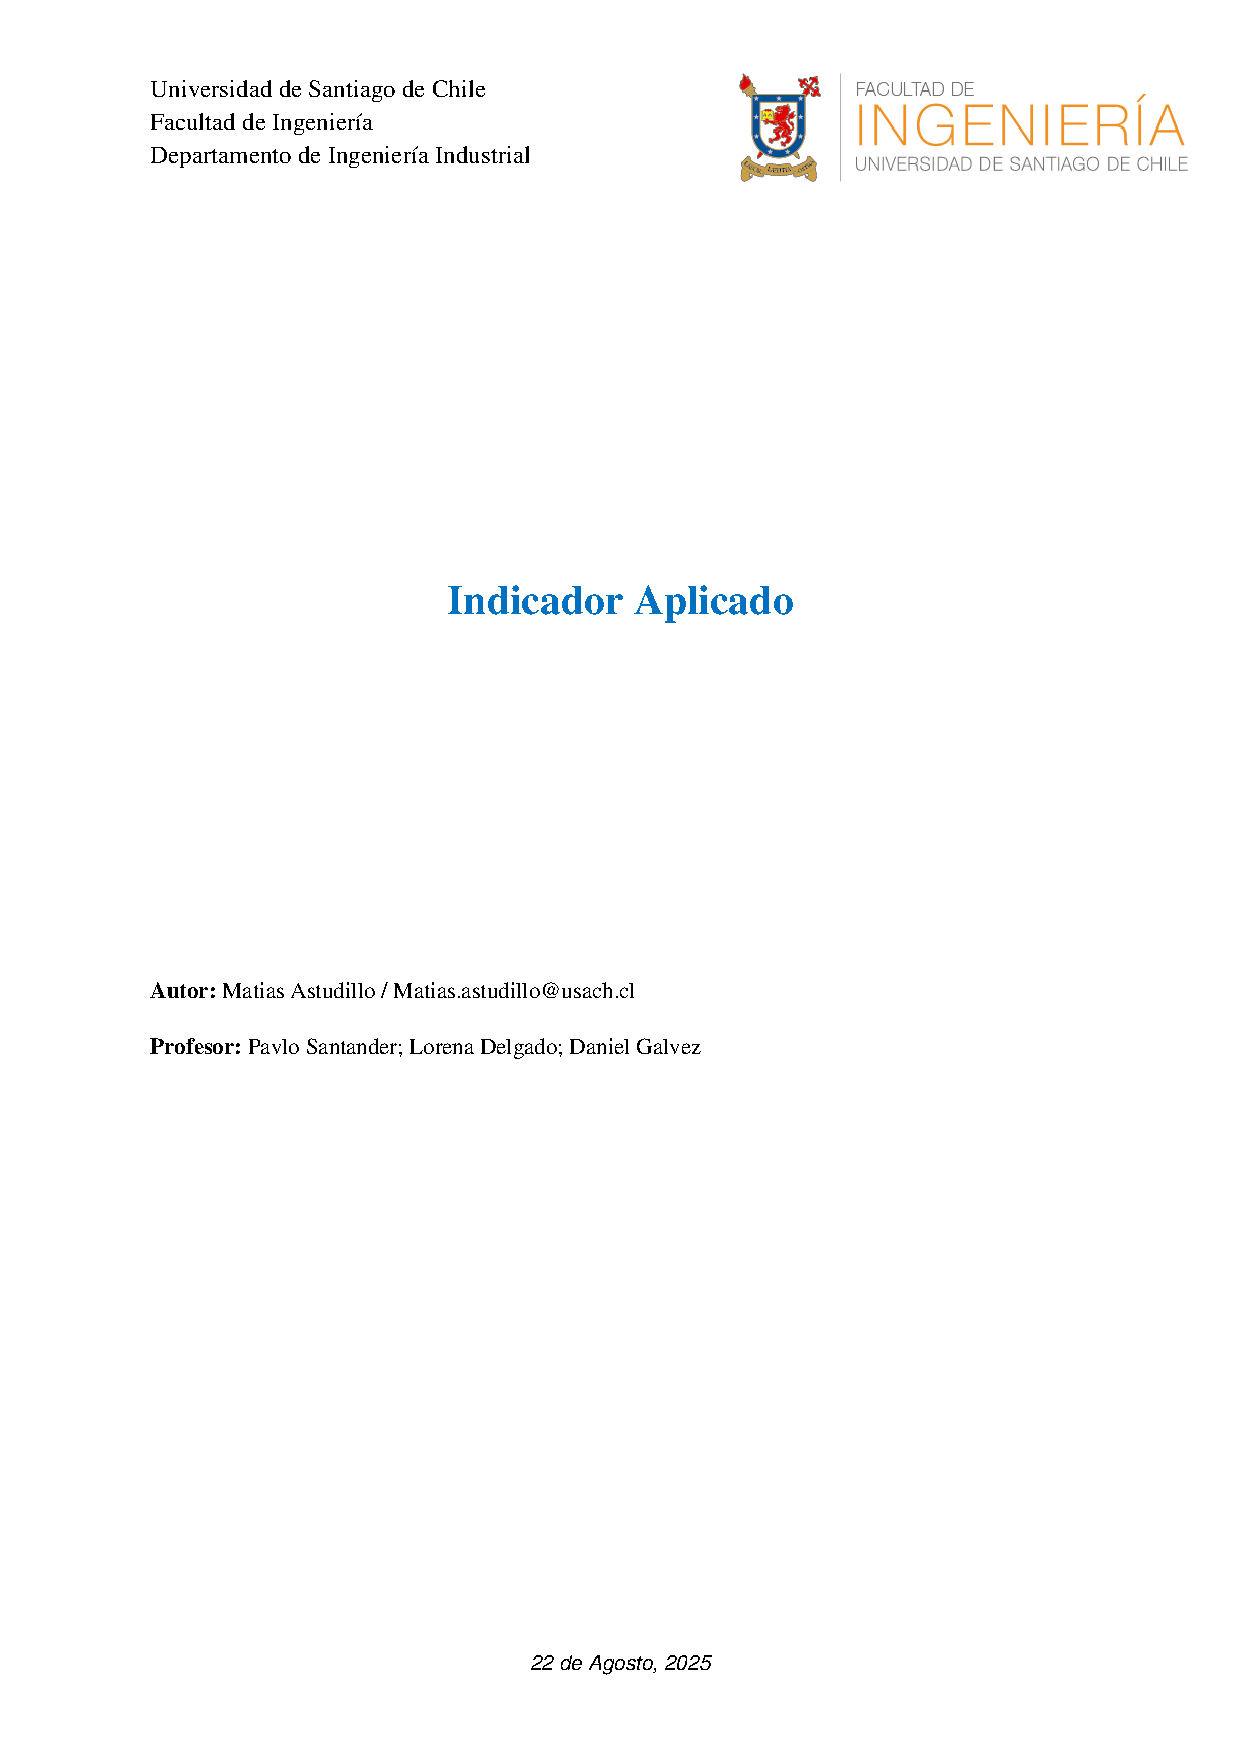
\includepdf[landscape=false, delta=2 2, frame=true,  
scale=0.8, offset=0 0cm, pagecommand*={\pagestyle{fancy} \section{Questionnaire for the Task 1.3}},
pagecommand={\pagestyle{fancy}},
nup=3x2,pages=-]{annex/1.3/Instrument.pdf}

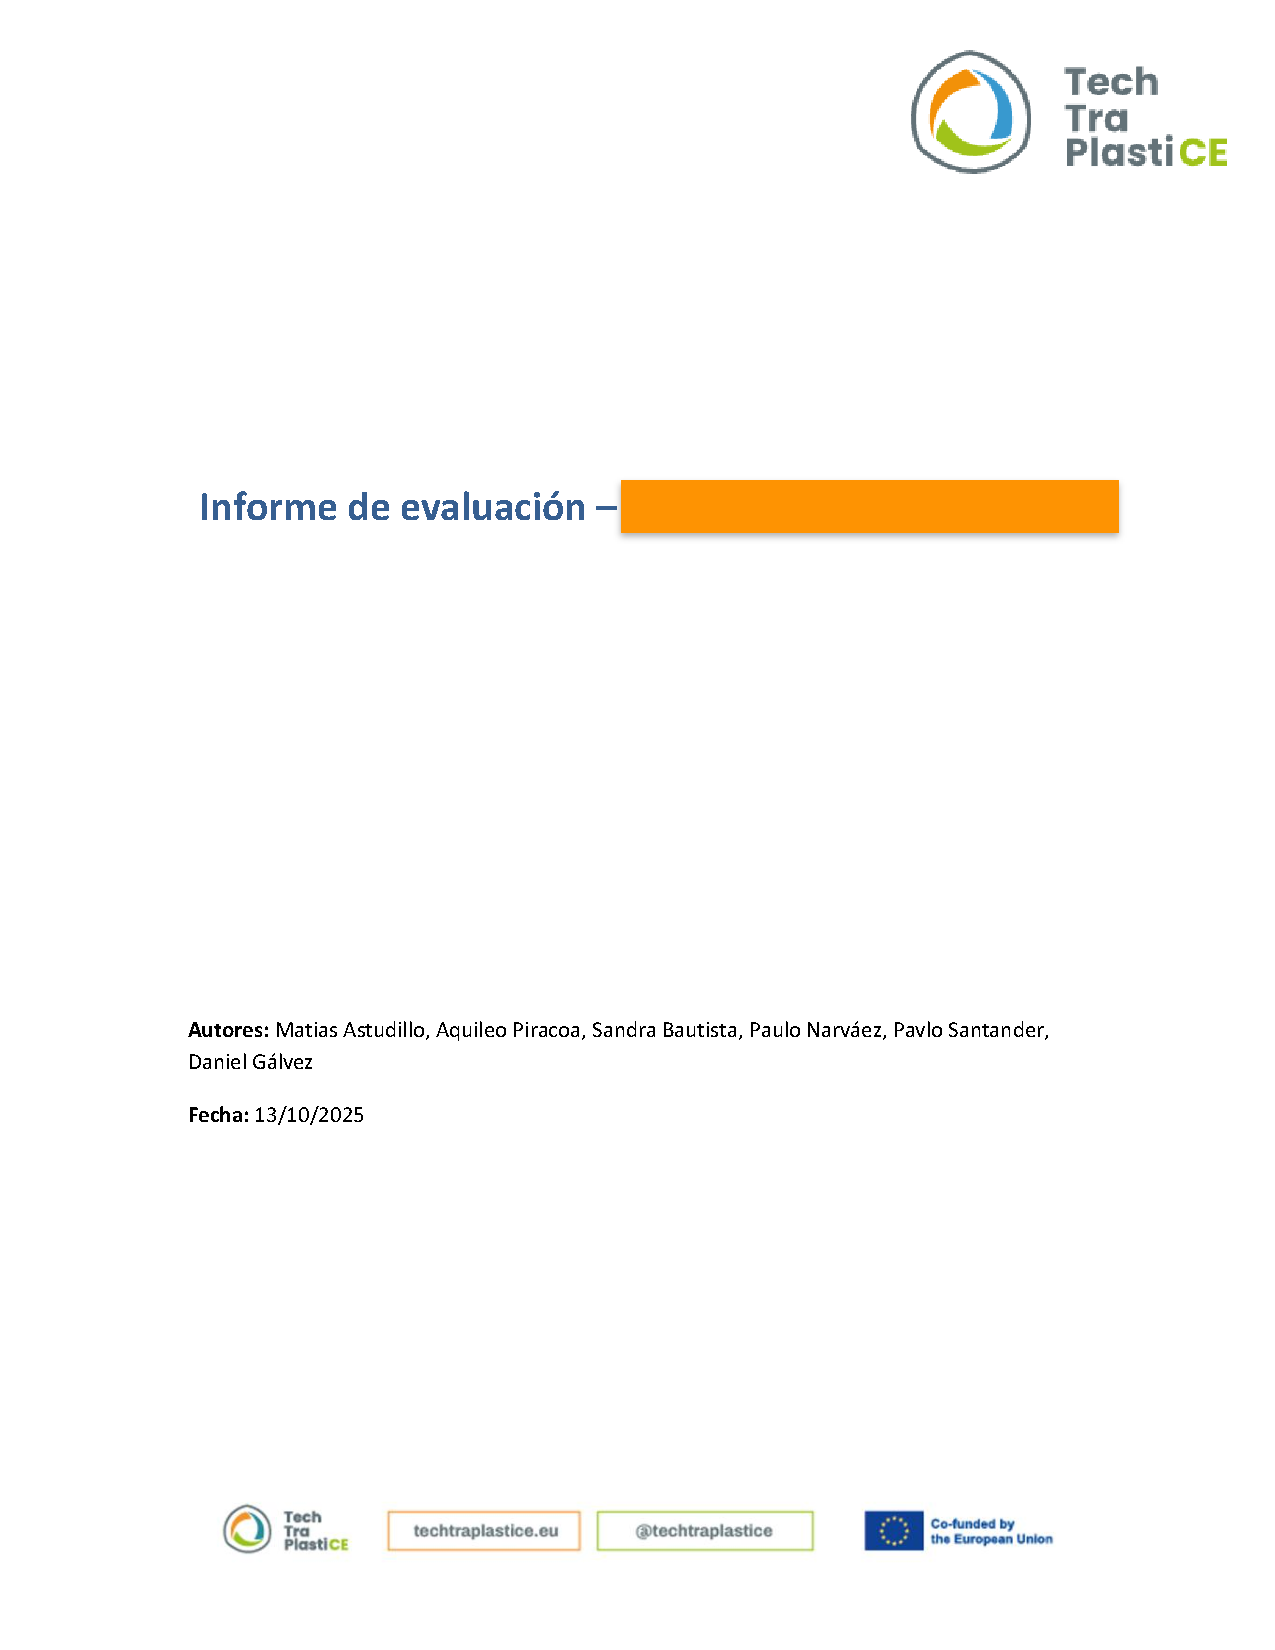
\includepdf[landscape=false, delta=2 2, frame=true,  
scale=0.75, offset=0 0cm, pagecommand*={\pagestyle{fancy} \section{Example of Rapport sent to the Companies}},
pagecommand={\pagestyle{fancy}},
nup=2x2, pages=-]{annex/1.3/Rapport-Example.pdf}


\backmatter


\end{document}
